\documentclass[12pt,twoside]{book}

\usepackage[a4paper,width=150mm,top=25mm,bottom=25mm]{geometry}
\usepackage[utf8]{inputenc}
\usepackage{xcolor}
\usepackage{graphicx}
\usepackage{amsmath}
\usepackage{url}
\usepackage{multicol}
\usepackage{amsfonts}
\usepackage[]{appendix}

\usepackage{tikz}
\usetikzlibrary{positioning,arrows}
\usetikzlibrary{decorations.pathmorphing}
\usetikzlibrary{decorations.markings}

\tikzset{
	fermion/.style={thick,draw=black, postaction={decorate}, decoration={markings,mark=at position 0.6 with {\arrow[black]{triangle 45}}}},
	photon/.style={decorate, draw=black, decoration={coil,aspect=0}},
	gluon/.style={decorate, draw=black, decoration={coil,amplitude=4pt, segment length=5pt}} 
}


\usepackage{hyperref}
\hypersetup{
	colorlinks,
	linkcolor= [RGB]{8 0 125},
	citecolor= [RGB]{8 0 125},
	urlcolor= [RGB]{8 0 125}
}

\usepackage{fancyhdr}
\pagestyle{fancy}
	\renewcommand{\chaptermark}[1]{ \markboth{#1}{} }
	\renewcommand{\sectionmark}[1]{ \markright{#1}{} }
	\fancyhead[LO, RE]{\thesection~ \rightmark}
	\fancyhead[RO,LE]{Chapter \thechapter}
	\fancyfoot[C]{\thepage}

\fancypagestyle{appendix}{
	\fancyhf{}
	\fancyhead[RO,LE]{Appendix \thechapter}
	\fancyfoot[C]{\thepage}
}

\fancypagestyle{acronymns}{
	\fancyhf{}
	\fancyhead[RO,LE]{Acronyms}
	\fancyfoot[C]{\thepage}
}

\fancypagestyle{bibliography}{
	\fancyhf{}
	\fancyhead[RO,LE]{Bibliography}
	\fancyfoot[C]{\thepage}
}




\usepackage[acronym, nopostdot, toc, nonumberlist]{glossaries}

\newglossary[for]{formulas}{forin}{forout}{Formulas}
\makeglossaries
\begin{acronym}[Bash]
	\acro{SM}{Standard Model of Particles Physics}
	\acro{QFT}{Quantum field theory}
	\acro{QED}{Quantum electrodynamics}
	\acro{QCD}{Quantum chromodynamics}
	\acro{LFV}{Lepton flavour violation}
	\acro{BSM}{Beyond the Standard Model of Particle Physics}
	\acro{LHC}{Large Hadron Collider}
	\acro{CMS}{Compact Muon Solenoid}
	\acro{TeV}{Tera electron volt, $1 \text{ TeV} = 1.6 \cdot 10^{-7}$ J}
	\acro{CERN}{European Organization for Nuclear Research, abbreviation from Conseil européen pour la recherche nucléaire}
	\acro{ATLAS}{A Toroidal LHC Apparatus}
	\acro{LHCb}{Large Hadron Collider beauty}
	\acro{ALICE}{A Large Ion Collider Experiment}
	\acro{PDF}{Parton density function}
\end{acronym}

\newglossaryentry{eta}{
	type={formulas},
	name={$\eta$}, 
	description={$= -\ln{\tan{\frac{\theta}{2}}}$}
}


\newglossaryentry{pT}{
	type={formulas},
	name={$p_{T}$}, 
	description={$= \sqrt{p_{x}^{2} + p_{y}^{2}}$}
}


\newglossaryentry{ETmis}{
	type={formulas},
	name={$\cancel{\vec{E}}_{T}$}, 
	description={$= - \sum_{i \in (1, .., n_{\text{meas.}})} \vec{p}_{T}^{i} $}
}

\newglossaryentry{dR}{
	type={formulas},
	name={$\Delta R$}, 
	description={$= \sqrt{(\Delta \phi)^{2} + (\Delta \eta)^{2}}$}
}

\glsaddall
\glsunsetall

\setlength{\parindent}{0pt}

\begin{document}


\newgeometry{centering}  
\begin{titlepage}
    \begin{center}
        \vspace*{1cm}
        
        \Huge
        \textbf{Lepton flavour violation in Z boson decays}
        
        \vspace{0.5cm}
        
        \large
        
        von
        
        \vspace{0.5cm}
	
	\textbf{B. Sc.}	
	
	\vspace{0.3cm}
        
        \textbf{David Brunner}
        
        \vspace{4.0cm}
        
        Masterarbeit in Physik
        
        \vspace{0.5cm}
        
        vorgelegt der 
        
        \vspace{0.5cm}
        
        Fakultät für Mathematik, Informatik und Naturwissenschaften der RWTH Aachen
        
        \vspace{0.5cm}
        
        im \today{}
        
        \vspace{0.5cm}
        
        angefertigt am
        
        \vspace{0.5cm}
        
        III. Physikalisches Institut B
        
        \vspace{0.5cm}
        
        bei 
        
        \vspace{0.5cm}
        
        Prof. Dr. Achim Stahl
    
    \end{center}
\end{titlepage}
\restoregeometry

\clearpage{\pagestyle{empty}\cleardoublepage}

\tableofcontents
\thispagestyle{empty}
\clearpage{\pagestyle{empty}\cleardoublepage}

\listoffigures
\thispagestyle{empty}
\addcontentsline{toc}{chapter}{List of figures}
\clearpage{\pagestyle{empty}\cleardoublepage}

\listoftables
\thispagestyle{empty}
\addcontentsline{toc}{chapter}{List of tables}
\clearpage{\pagestyle{empty}\cleardoublepage}

\chapter{Theoretical basics about the Standard Model and lepton flavour violation}
The Standard Model of Particle Physics (SM) is the description of the physics of elementary particles and their interaction, which is known up now. The theoretical foundation is the perturbative quantum field theory (QFT) which is harmonised with Special Relativity. In the formaslim of QFT classical fields are quantized and the information of the interaction of the particles is encoded in the lorentz-invariant lagrangian density $\mathcal{L}$. 

\section{Particles and interactions}
\label{section_1_1}

In the SM elemental particles can be characzerized by their spin, which is a quantum number describing a analogon to the intrinsic angular momentum. Fermions carry spin $\frac{1}{2}$ and are represented by Dirac spinors $\psi$, which are complex 4-component objects defined through their behaviour under Lorentz transformation: $\psi^{\alpha}(x) \rightarrow S[\Lambda]^{\alpha}_{\beta} \psi^{\beta}(\Lambda^{-1}x)$. The interaction between the fermions are described by gauge symmetries, which are local symmetry transformations, leaving the langrangian invariant with the introduction of a gauge boson. Gauge boson are elemental particles with spin 1. All relevant symmetries and the corresponding interaction are described in the following, the list of all elemental particle and their properties are listed in table \ref{tab:1.1}.

\subsection*{\small U(1)${_e}$ symmetry and quantum electrodynamics (QED)}

The free langrangian of a fermion using the Dirac spinors, using $\gamma^{\mu}$ as the gamma matrizes and $\bar{\psi} = \psi^{\dagger}\gamma^{0}$, can be written as:

\begin{equation}
	\mathcal{L}_{0} =  i\bar{\psi}(x)\gamma^{\mu}\partial_{\mu}\psi(x) - m\bar{\psi}(x)\psi(x)
\end{equation}

Performing a global transformation of the the kind $\psi(x) \rightarrow \psi'(x) = e^{iQ\alpha}\psi(x)$, with Q and $\alpha$ as real constants, the langrangian stays invariant under this so called U(1) transformation. The invariance is not fullfilled if $\alpha$ depends explictly on the spacetime $x$ and is called a local gauge transformation. To insure invariance under a gauge transformation, a new 4-component lorentz vector field $A_{\mu}(x)$ is introduced with following property under U(1) transformation: $A_{\mu} \rightarrow A'_{\mu}(x) = A_{\mu}(x) + \frac{1}{e}\partial_{\mu}\alpha(x)$. Using the definition of the covariant derivate $D_{\mu} = \partial_{\mu} - ieQA_{\mu}(x)$, the following langrangian stays invariant under local U(1) transformation:

\begin{equation}
	\mathcal{L} = i\bar{\psi}(x)\gamma^{\mu}D_{\mu}\psi(x) - m\bar{\psi}(x)\psi(x) = \mathcal{L}_{0} + eQA_{\mu}(x)\bar{\psi}(x)\gamma^{\mu}\psi(x)
\end{equation}

With the gauge transformation the gauge boson of the electromagnetic interaction is introduced, which couples to the fermions with electric charge e: the photon $\gamma$.


\subsection*{\small SU(3)${_C}$ symmetry and quantum chromodynamics (QCD)}

Beside the electric charge, the so-called quarks are fermions carrying the one of three possible color charges (denoted with r,b,g). Labeling the quark spinor with color $c$ as $q^{c} = \psi_{q}(c)$ and putting them all into a three vector with quark $q_{f} = (q^{b}, q^{r}, q^{g})$, the free lagrangian of quarks can be written as

\begin{equation}
	\mathcal{L}_{0} = \sum_{f} \bar{q_{f}}(i\gamma^{\mu}\partial_{\mu} - m_{f})q_{f}
\end{equation}

The index $f$ denotes the flavour of the quark is explained below. Like in the QED example a local gauge theory exists, which introduces gauge bosons. A transformation of the kind $q_{f} \rightarrow q'_{f} = e^{i\frac{\lambda^{a}}{2}\alpha_{a}(x)} q_{f}$, with $\frac{1}{2} \lambda^{a}$ as non communting 3x3 matrixes and $a \in (1, 2, .., 8)$, is a local SU(3)$_{C}$ transformation. To get a lagrangian invariant under this tranformation, 8 new gauge bosons $G^{\mu}_{a}(x)$, so-called gluons have to be introduced, corresponding to the number of generators $\lambda^{a}$ to represent the SU(3)$_{C}$ algebra. Defining the covariant derivative $D_{\mu} = \partial_{\mu}-ig_{s}\frac{\lambda^{a}}{2}G^{\mu}_{a}(x)$ and demand the gluons to transform using $U = e^{i\frac{\lambda^{a}}{2}\alpha_{a}(x)}$ like $G^{\mu}_{a}(x) \rightarrow G^{\mu}(x)' = UG^{\mu}U^{\dagger} - \frac{i}{g_s}(\partial^{\mu}U)U^{\dagger}$ the invariant lagrangian of QCD can be written like 

\begin{equation}
	\mathcal{L} = \sum_{f} \bar{q_{f}}(i\gamma^{\mu}D_{\mu} - m_{f})q_{f}
\end{equation}


\subsection*{\small SU(2)$_{W}$ x U(1)$_{Y}$, the electroweak interaction and Higgs mechanism}

The flavour of fermions is a quantum number describing of the type particle. For the quarks six different flavours (up, down, charm, strange, top, bottom) exist, for the color-less leptons/neutrinos fermions the three lepton flavour (electron, muon, tau) exist. Also a important quantity is the chirality, because in the electroweak theory not all chirality configuration of the fermions couples to the gauge bosons. We define the spinors of fermions with lefthanded(L) or righthanded(R) chirality with $\psi_{L/R} = \frac{1}{2}(1\mp \gamma^{5})\psi$ and for simplizity looking only at the first generation of quarks/leptons, the spinor of quarks/leptons are defined as $u = \psi_{u}, d = \psi_{d}, e = \psi_{e}, \nu = \psi_{\nu_{e}}$. If the fermions are assembled as $q_{L} = (u_{L}, d_{L}), u_{R}, d_{R}, l_{L} = (e_{L}, \nu_{L}), e_{R}$ and consindering them to be massless, the free langrangian of the electroweak theory is


\begin{equation}
	\mathcal{L}_{0} = i\bar{q}_{L}\gamma^{\mu}\partial_{\mu}q_{L} + i\bar{l}_{L}\gamma^{\mu}\partial_{\mu}l_{L} + \sum_{f \in (e, u, d)} i\bar{f}_{R}\gamma^{\mu}\partial_{\mu}f_{R}
\end{equation}

The local SU(2)$_{W}$ x U(1)$_{Y}$ gauge transformation, which is a tranformation of the kind


\begin{equation}
	\begin{split}
		q_{L} \rightarrow q'_{L} = e^{iQ_{q} \alpha_{Y}(x)} e^{i\frac{\sigma_{j}}{2}\alpha^{j}_{W}(x)}q_{L} \\
		l_{L} \rightarrow l'_{L} = e^{iQ_{l} \alpha_{Y}(x)} e^{i\frac{\sigma_{j}}{2}\alpha^{j}_{W}(x)}l_{L} \\
		f_{R} \rightarrow f'_{R} = e^{iQ_{f} \alpha_{Y}(x)}, \quad f \in (e, u, d)
	\end{split}			
\end{equation}


with $\sigma_{j}, j \in (1,2,3)$ as the Pauli matrices, $Q$ as real constant and $a_{Y}, a^{j}_{W}$ as real function of spacetime, introduces 4 gauge bosons, the three $W^{j}_{\mu}(x)$, origating from SU(2)$_{W}$, and the $B_{\mu}$ from U(1)$_{Y}$. Using $U_{L} = e^{i\frac{\sigma_{j}}{2}\alpha^{j}_{W}(x)}$, demanding the transformation properties $B_{\mu} \rightarrow B'_{\mu} = B_{\mu} + \frac{1}{g'}$, $W'_{\mu} \rightarrow U_{L}\frac{\sigma_{j}}{2}W_{\mu}^{j}U_{L}^{\dagger} - \frac{i}{g}(\partial_{\mu}U_{L})U_{L}^{\dagger}$ and defining the covariante derivate 

\begin{equation}
	\begin{split}
		D^{q}_{\mu} = \partial_{\mu}  - ig\frac{\sigma_{j}}{2}W^{j}_{\mu} - ig'Q_{q}B_{\mu} \\
		D^{l}_{\mu} = \partial_{\mu}  - ig\frac{\sigma_{j}}{2}W^{j}_{\mu} - ig'Q_{l}B_{\mu} \\
		D^{f_R}_{\mu} = \partial_{\mu}  - ig'Q_{f}B_{\mu}, \quad f \in (e, u, d)
	\end{split}
\end{equation}

the gauge invariant lagrangian of the electroweak can be written as 

\begin{equation}
	\mathcal{L} = i\bar{q}_{L}\gamma^{\mu}D_{\mu}^{q}q_{L} + i\bar{l}_{L}\gamma^{\mu}D_{\mu}^{l}l_{L} + \sum_{f \in (e, u, d)} i\bar{f}_{R}\gamma^{\mu}D^{f_R}_{\mu}f_{R}
\end{equation}

The problem from this formulation arises from the fact, that the gauge bosons and fermions are measured to have a mass. To explain this discrepancy the Higgs mechanism is introduced. Considering a complex scalar field doublet $\Phi(x) = (\phi^{1}(x), \phi^{2}(x))$, which transform under SU(2)$_{W}$ like $\Phi(x) \rightarrow \Phi'(x) = e^{iQ_{\Phi} \alpha_{Y}(x)} e^{i\frac{\sigma_{j}}{2}\alpha^{j}_{W}(x)}\Phi(x)$ the lagrangian can be written as

\begin{equation}
	\mathcal{L}_{H} = i\bar{q}_{L}\gamma^{\mu}D_{\mu}^{q}q_{L} + i\bar{l}_{L}\gamma^{\mu}D_{\mu}^{l}l_{L} + \sum_{f \in (e, u, d)} i\bar{f}_{R}\gamma^{\mu}D^{f_R}_{\mu}f_{R}
\end{equation}

\clearpage{\pagestyle{empty}\cleardoublepage}

\chapter{Experimental set up}
In this thesis the data, which is analyzed for the search of \gls{LFV} in Z boson decays, is produced by proton-proton-collisions of the Large Hadron Collider (\gls{LHC}) \cite{LHC} and recorded by the Compact Muon Solenoid (\gls{CMS}) \cite{CMS} in the year of 2016. Both apparatus are explained in the sections \ref{sec:section_2_1} and \ref{sec:section_2_2} respectively and proton physics is explained in section \ref{sec:section_2_1_2}.


\section{Large Hadron Collider}
\label{sec:section_2_1}

The \gls{LHC} is a circular proton-proton-collider with a center of mass energy of $\sqrt{s} = 13$ TeV \cite{LHC2}, which is located at the European Organization for Nuclear Research (\gls{CERN}) in Geneva. A schematic overview of the acceleration system is shown figure \ref{fig:fig_2_1}. The acceleration of the protons is done by a system of pre-accelerators, which feeds the protons then in the \gls{LHC}, where they are further accelerated to reach the designed center of mass energy. \\

\begin{figure}[ht]
	\centering
	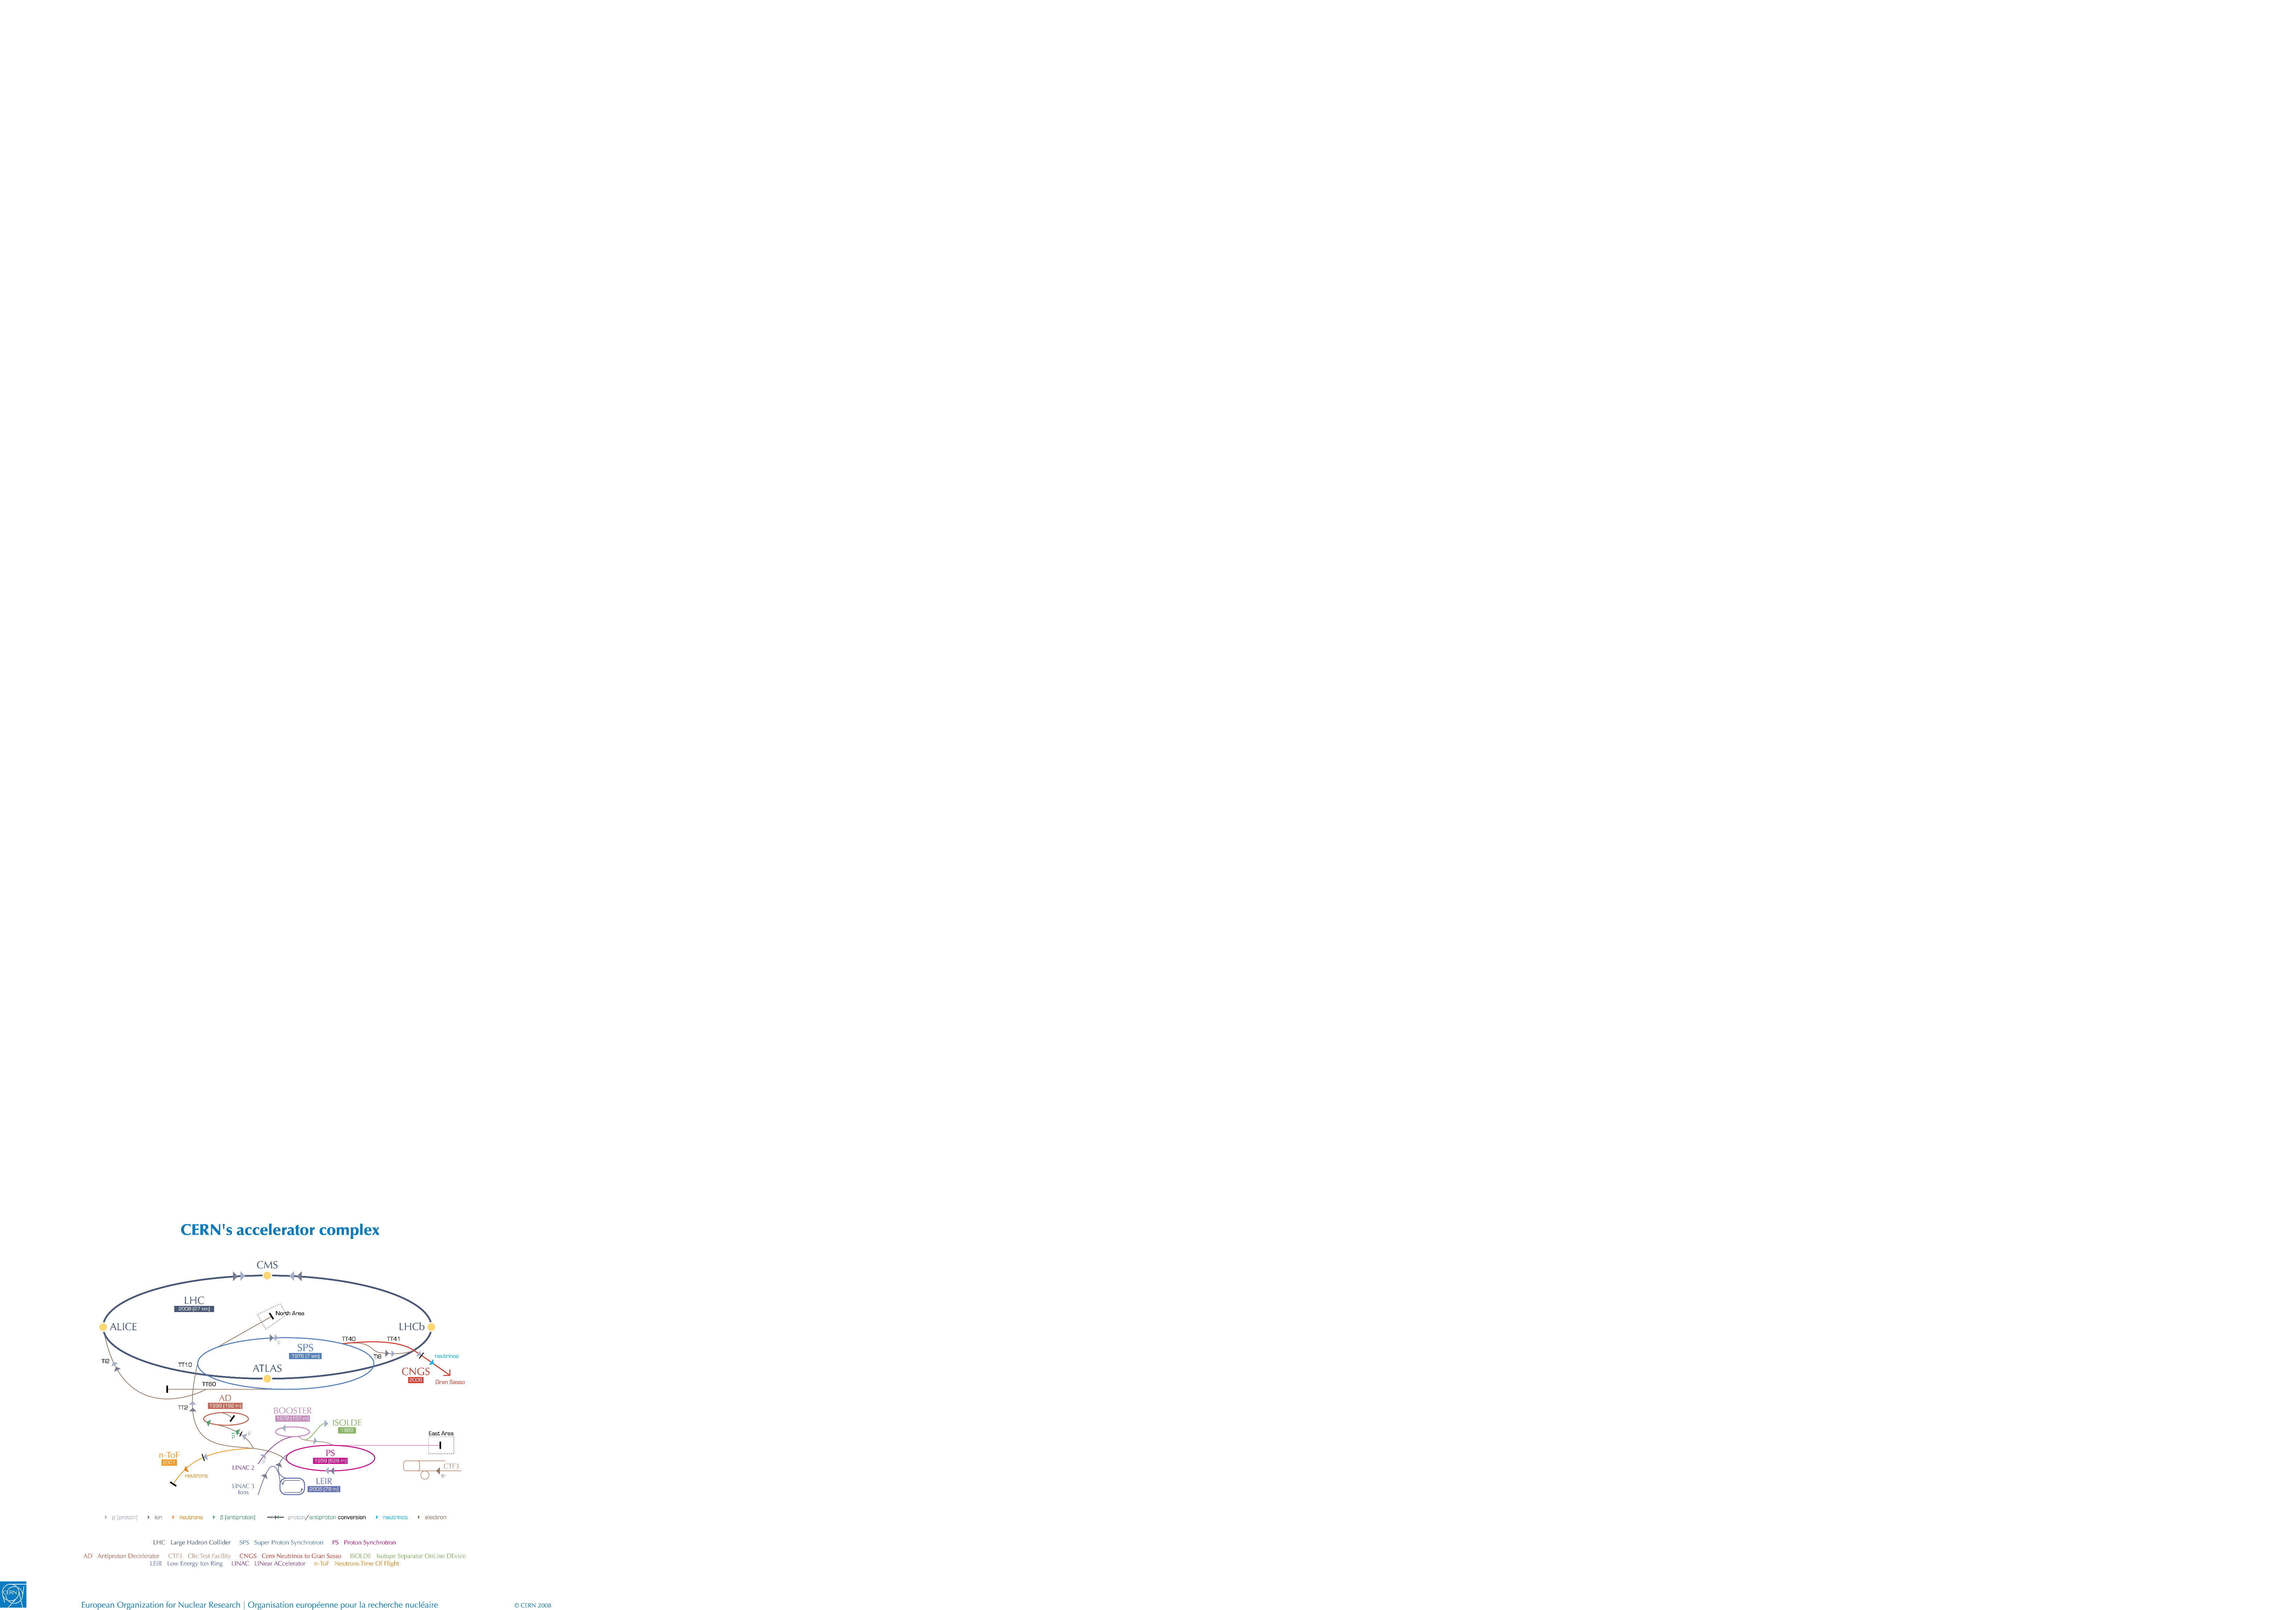
\includegraphics[width=1.0\textwidth]{pictures/LHC.pdf}

	\caption[Schematic overview of CERN accelerator complex]{Schematic overview of \gls{CERN} accelerator complex, including the \gls{LHC} and the previous pre-accelerators. The yellow points mark the position of the particles detectors at the collisions points. Taken from \cite{LHCACCL}.}
	\label{fig:fig_2_1}
\end{figure}

At each collision point of the proton beams a sophisticated detector is installed, indicated by the yellow dots in figure \ref{fig:fig_2_1}. The design of each of these detectors is optimized to a certain physics program. The four big experiments are the \gls{CMS} and A Toroidal LHC Apparatus (\gls{ATLAS}) \cite{ATLAS}, which are designed to probe \gls{SM} and \gls{BSM} physics, the Large Hadron Collider beauty (\gls{LHCb}) \cite{LHCb}, which is designed for decays of hadrons involving bottom quarks, and the A Large Ion Collider Experiment (\gls{ALICE}) \cite{ALICE}, which is designed for heavy ion collisions.


\subsection{Properties of the proton beams}
\label{sec:section_2_1_1}

The protons in the \gls{LHC} are accelerated in bunches, which contain around $10^{11}$ protons, and are separated in space by a time interval of 25 ns \cite{LHCSTATS}. The size of the bunches is oscillating due to dynamics of the charged protons in the magnetic system of the \gls{LHC} \cite{LHC}. The beam size can be parametrized by the emittance $\epsilon$, which describes the spread of the beam particles in the spatial and momentum phase space, and the $\beta$ function, which describes the oscillation amplitude \cite{BEAMPHY}. The properties of the beam have a high impact on the quality of the collider, which is parametrized by instantaneous luminosity $\mathcal{L}$ \cite{Luminosity}

\begin{equation}
	\label{eq:eq_2_1}
	\mathcal{L} = \frac{\gamma \cdot f \cdot k_{b} \cdot n_{1} \cdot n_{2}}{4 \cdot \pi \cdot \epsilon \cdot \beta}
\end{equation} 

with Lorentz gamma factor $\gamma$, the revolution frequency $f$ of the bunches, the number of colliding bunches $k_{b}$ and the number of protons $n_{i}$ in each bunch. There is a direct dependence of rate of collision events $\frac{dN}{dt}$ to the luminosity, and the total number of collision events $N$ to the integrated luminosity $\mathcal{L}_{int}$

\begin{equation}
	\label{eq:eq_2_2}
	\begin{split}
		\frac{dN}{dt} = \sigma \cdot \mathcal{L} \\
		N = \sigma \cdot \mathcal{L}_{int}
	\end{split}
\end{equation}	

with $\sigma$ as the cross section of of a certain process in proton-proton collisions. So the beam parameter have a direct influence on the total number of possible recorded events and the amount statistics which is provided for the analysis. Figure \ref{fig:fig_2_2} shows of the collected integrated luminosity as a function of time during  data-taking run in 2016. 

\begin{figure}[ht]
	\centering
	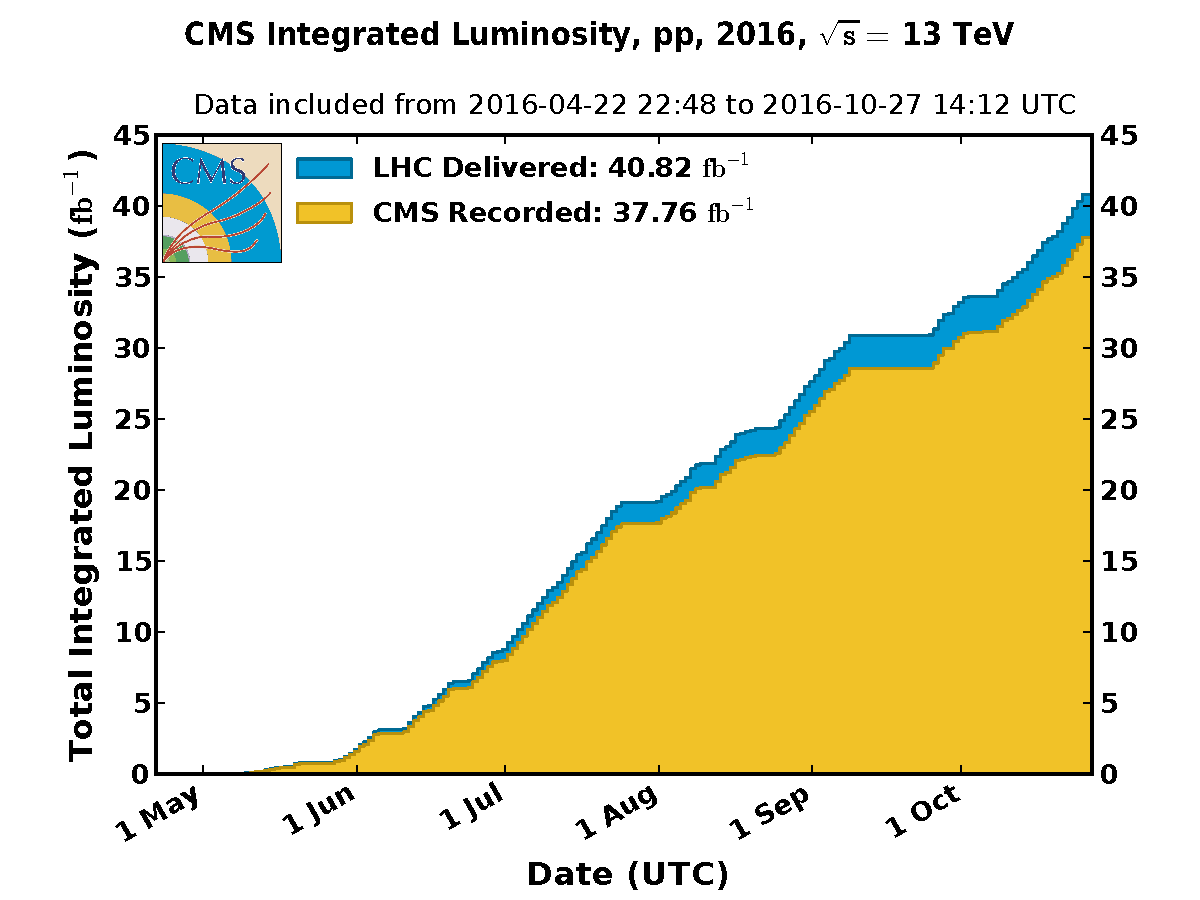
\includegraphics[width=0.7\textwidth]{pictures/int_lumi_per_day_cumulative_pp_2016.pdf}

	\caption[Total integrated luminosity of the year 2016]{Total integrated luminosity collected by \gls{CMS} as a function of time in the run in the year 2016, taken from \cite{CMSLUMI}}
	\label{fig:fig_2_2}
\end{figure}


\subsection{Proton-proton collisions}
\label{sec:section_2_1_2}

Protons are non-elementary hadrons, which are a bound state of three quarks, in this case of two up-quarks and one down-quark. This bound state can be described by \gls{QCD}, see section \ref{sec:section_1_1_2}, and give rise to the quark-parton model \cite{Peskin}. In this description protons are composite of the partons, which are beside the three quarks of the bound state, other quarks and gluons which are produced/annihilated during the interaction in the bound state. Each of the quarks and gluons carry a fraction $x_{i}$ of the total momentum $P$ of the proton, and the probability of an existing parton with flavour f, with $f \in (u, d, \bar{u}, \bar{d}, ... g)$ and with $x_{i}$ is described by the parton density function (\gls{PDF}) $f_{f}(x)$ \cite{Peskin, PDF1}. \gls{PDF} are not predictable by \gls{QCD} and have to be measured in deep inelastic scattering processes. As an example, figure \ref{fig:fig_2_3} shows the measurement of the \gls{PDF} in the ZEUS experiment \cite{ZEUS}. \\

\begin{figure}[ht]
	\centering
	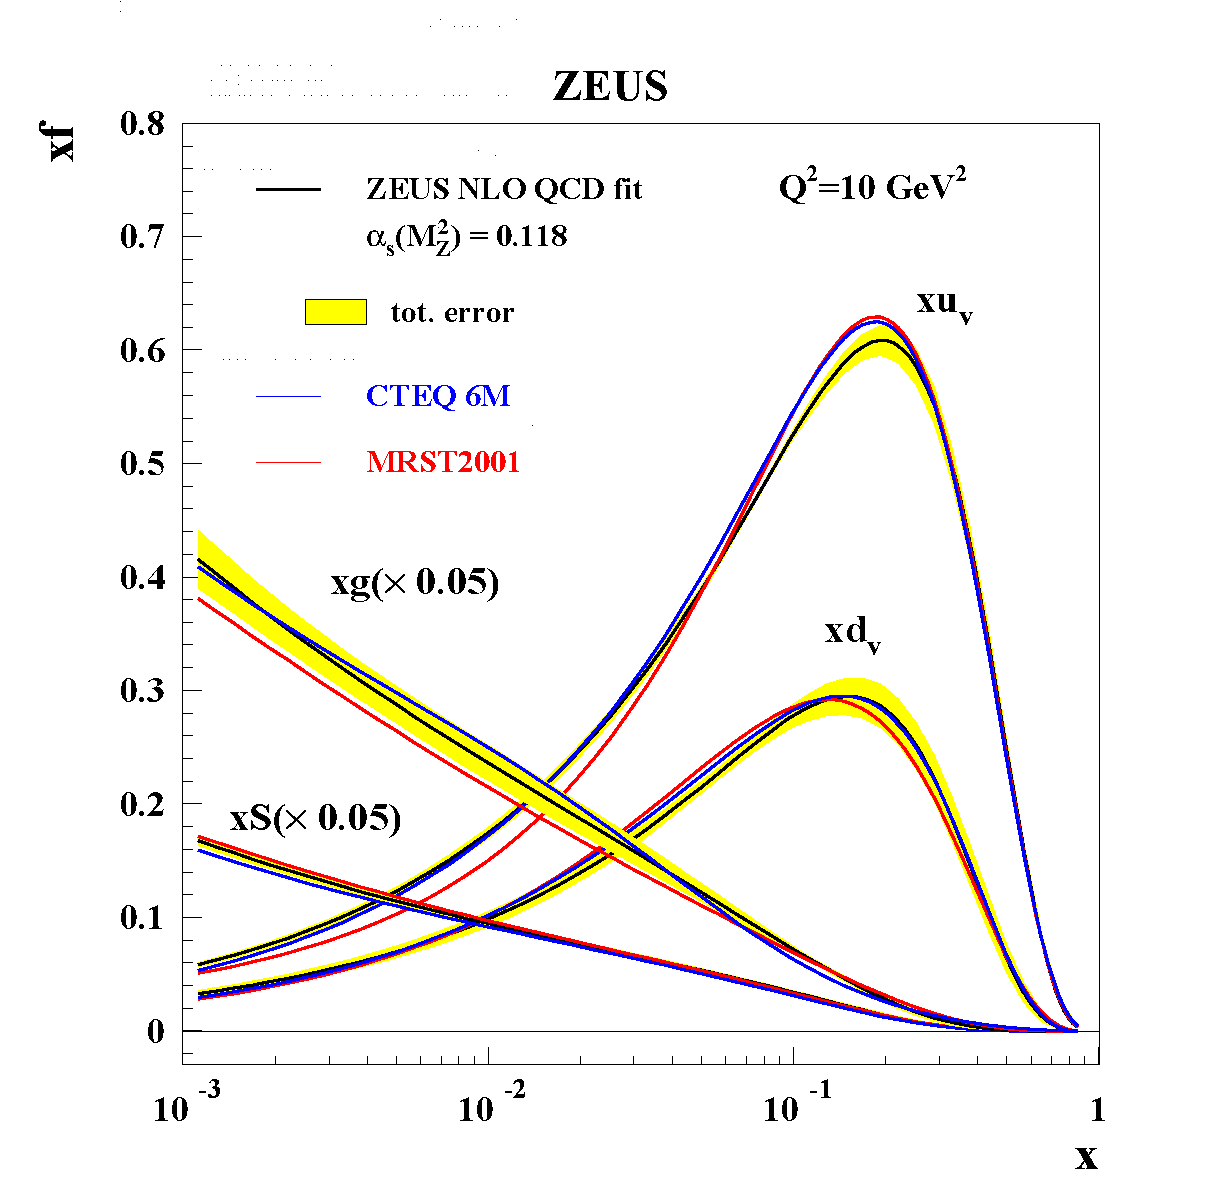
\includegraphics[width=0.7\textwidth]{pictures/ZEUS_PDF.pdf}

	\caption[Proton \gls{PDF} from ZEUS]{\gls{PDF} of up-quarks, down-quarks and gluons in a proton measured by the ZEUS experiment, taken from \cite{PDFMEAS}. The measurement shows that $u$ and $d$ quarks, which are in the bound state of the proton, have a high probability to carry a large fraction of the proton momentum. Other quarks and gluons have a high probability to carry a low momentum fraction of the proton.}
	\label{fig:fig_2_3}
\end{figure}

In collisions of the protons at the \gls{LHC} the cross sections of the different processes depend on the \gls{PDF} and the $x_{i}$ of the partons. Taking as example proton-proton collisions into fermion pair production, two quarks with momentum $x_{1}P$ and $x_{2}P$ will produce the fermion pair, all the other constituent $X$ are not participating in the interaction and carry away the remaining proton momenta, see figure \ref{fig:fig_2_4} for a schematic example. The cross section $\sigma(pp\to f\bar{f} + X)$ \cite{Peskin} for such a process can be calculated with 

\begin{equation}
	\label{eq:eq_2_3}
	\sigma(pp\to f\bar{f} + X) = \int_{0}^{1}dx_{1}\int_{0}^{1}dx_{2}\sum_{f \in (u, d, \bar{u}, \bar{d}, ... g)} f_{f}(x_{1})f_{\bar{f}}(x_{2}) \cdot \sigma(q_{f}(x_{1})q_{\bar{f}}(x_{2}) \to f\bar{f}). 
\end{equation}


\begin{figure}[ht]
	\centering
	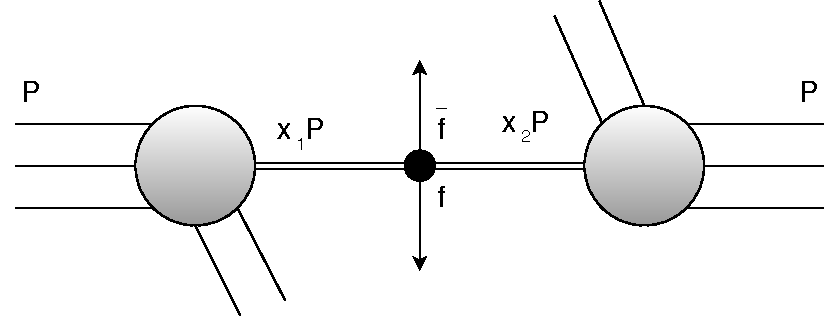
\includegraphics[width=0.7\textwidth]{pictures/ppcollision.pdf}

	\caption[Sketch of proton-proton collision]{Sketch of a proton-proton collision at the \gls{LHC}. The protons have momentum $P$, the quarks involved in the interaction have the fraction $x_{i}$ of it, all other rest carries away the remaining momenta}
	\label{fig:fig_2_4}
\end{figure}


\section{Compact Muon Solenoid}
\label{sec:section_2_2}

The \gls{CMS} is a multi-purpose, multi-functional particle detector. The detector consists of several layers, which have each its functionality and purpose for the detection of particles. This design enables the measurement of kinematic properties of the particles produced in each scattering event, like momenta/energy/angular distributions, and the identification of the particles. Figure \ref{fig:fig_2_5} shows the \gls{CMS} profile with all detector layers, which are explained in section \ref{sec:section_2_2_2}, and the interactions of different particle species in the detector, which are explained in section \ref{sec:section_2_2_4}.

\begin{figure}[ht]
	\centering
	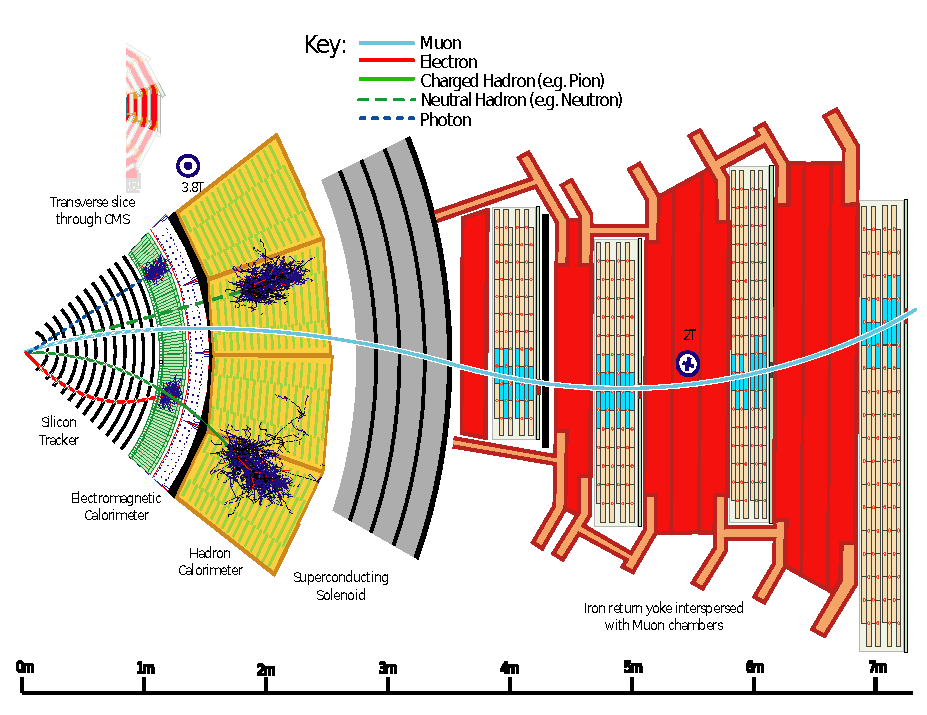
\includegraphics[width=0.7\textwidth]{pictures/CMS.pdf}

	\caption[Profile of CMS detector]{Sketch of the profile of \gls{CMS} with detectors and several particle species and their interactions in the detectors, taken from \cite{PARTICLEFLOW}}
	\label{fig:fig_2_5}
\end{figure}


\subsection{Coordinate convention}

The coordinate system is set to have the origin centered at the nominal collision point of the detector, with the x-axis pointing into the direction of the center of \gls{LHC}, the y-axis is pointing upwards into direction of the sky and z-axis points into the direction of the beam pipe. The coordinate system is choosen in a way, that the azimuthal angle $\phi$ is measured in the x-y plane, and the polar angle $\theta$ is measured from the z-axis. Instead of the polar angle $\theta$, in general the pseudo rapidity \gls{eta} $= -\ln{\tan{\frac{\theta}{2}}}$ is used due to the invariance under lorentz boost of $\Delta$\gls{eta} of two objects in the high energy limit.


\subsection{Sub-detectors of \gls{CMS}}
\label{sec:section_2_2_2}

\subsection*{Tracker system}

The most inner part of \gls{CMS} is the silicon tracker \cite{CMS2, CMSTRACKER}. Its inner part is the pixel detector, which is cylindrical around the beam. Figure \ref{fig:fig_2_6} shows the layout of the pixel detector. It consists of three layers in the barrel, which are located at the radial distance of 4.4 cm, 7.3 cm, 10.2 cm and have a length of 53 cm, and two turbine shaped layers on each side of the barrel, which are located $|z| = 34.5/46.5$ cm and have a radial expansion of 6 to 15 cm. All in all $66\cdot 10^{6}$ pixels with a size of 100 x 150 $\mu$m$^{2}$ are implemented in the pixel detector. The precision of the space point measurement of a crossing charged particle is about 10 $\mu$m in the $r-\phi$ direction and 20 $\mu$m in the z direction. \\

\begin{figure}[ht]
	\centering
	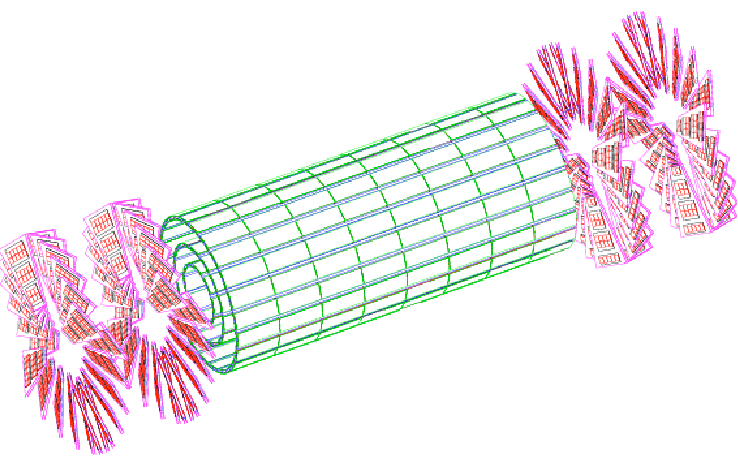
\includegraphics[width=0.7\textwidth]{pictures/CMS_tracker.pdf}

	\caption[Pixel detector layout of CMS]{Pixel detector layout of CMS, taken from \cite{CMS2}}
	\label{fig:fig_2_6}
\end{figure}


The outer part of the tracker is the silicon strip detector as shown in figure \ref{fig:fig_2_7}. The strip detector is spaced in cylindric layers around the beam pipe and is divided into an inner/outer barrel and the inner disc and endcap. The inner barrel is made of 4 layers with a coverage in z direction up to 65 cm in each direction, with a strip thickness of 320 $\mu$m and a $r-\phi$ resolution of 23-34 $\mu$m and z resolution of 23 $\mu$m. The outer barrel includes six layers with a strip thickness of 500 $\mu$m, a coverage in z direction up to 110 cm and a $r-\phi$ coordinate resolution of 35-52 $\mu$m and z coordinate resolution of 52 $\mu$m. The endcap are nine disc-like layers on each side in z direction, occupying the space in the range 120 cm $< |z| < $ 280 cm, the inner discs are arranged in 3 layers and fill the gap between barrel and endcap. In total a region up to $|$\gls{eta}$|$ $< 2.5$ is covered by the complete strip detector. \\

\begin{figure}[ht]
	\centering
	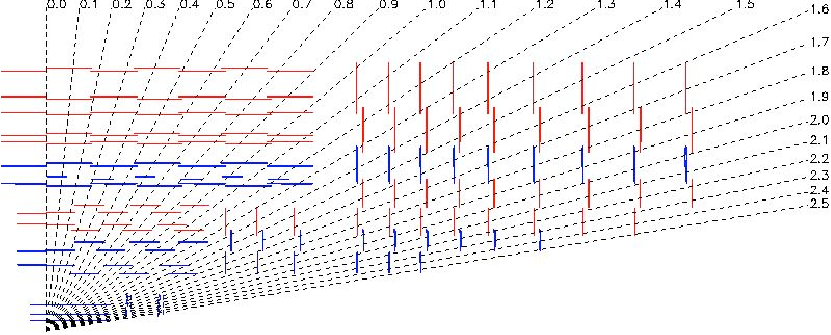
\includegraphics[width=1\textwidth]{pictures/CMS_strip.pdf}
	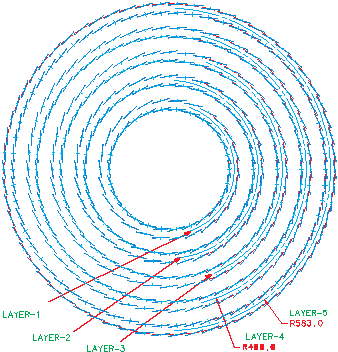
\includegraphics[width=0.5\textwidth]{pictures/CMS_strip2.pdf}

	\caption[Strip detector of CMS]{The first subfigure shows the layout in a z-view, where the numbers give the $\eta$ region. The second subfigure shows a transverse view of the barrel strip detector, taken from \cite{CMS2, ECAL}}
	\label{fig:fig_2_7}
\end{figure}

\subsection*{Calorimeter}

Outside the tracker two calorimeters are installed. The electromagnetic calorimeter (\gls{ECAL}) \cite{CMS2, ECAL} is built up by 61200 lead tungstate (\gls{PbWO4}) crystals in the barrel part and 7324 crystals in the endcap. Figure \ref{fig:fig_2_8} shows the schematic view of the \gls{ECAL}. The barrel region covers a region from 0 $<$ $|$\gls{eta}$|$ $<$ 1.479, in which each crystal have the dimensions of 22 mm x 22 mm x 230 mm. The endcap region covers to remaining part of 1.479 $<$ $|$\gls{eta}$|$ $<$ 3.0, in which the crystals have a dimension of 28.6 mm x 28.6 mm x 220 mm. In $r$ direction the barrel region is located at a distance to the beam pipe of 129 cm, the endcap region is located at a distance of 314cm. For the readout the scintillation light, due to of energy deposition of the particles in the barrel region silicon avalanche photo-diodes are used, in the endcap vacuum phototrides are used. The energy resolution of the \gls{ECAL} is given by

\begin{equation}
	\label{eq:eq_2_4}
	\frac{\sigma}{E} = (\frac{3.63 \sqrt{\text{MeV}}}{\sqrt{E}})^2 + (\frac{124 \text{MeV}}{\sqrt{E}})^2 + 0.26^{2}
\end{equation}

and measured for supermodules, which group 4 modules, which contains 500 crystals each. \\

\begin{figure}[ht]
	\centering
	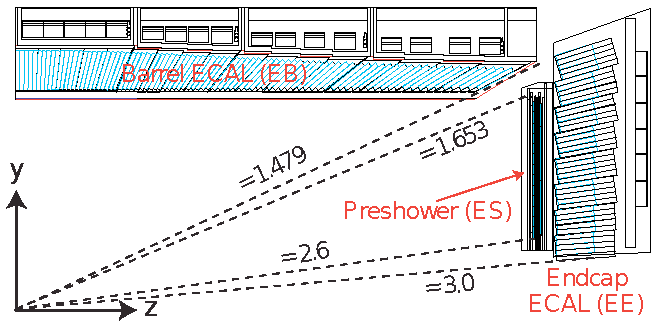
\includegraphics[width=1\textwidth]{pictures/CMS_ElectromagneticCalorimeter.pdf}

	\caption[Electromagnetic calorimeter of CMS]{Schematic view of the \gls{ECAL}, taken from \cite{CMS2}}
	\label{fig:fig_2_8}
\end{figure}

The second calorimeter is the hadronic calorimeter (\gls{HCAL}) \cite{CMS2, HCAL}. It is build up by wedges made of brass absorber plates, orientated parallel to the beam axis, with plastic scintillators between each absorber plate. The placement of absorber/scintillator is alternating, in total 17 layers of active scintillator material are placed, which are connected with a wavelength shifting fiber, forming so-called towers. The readout of the optical signal from the HCAL towers is done by pixelated hybrid photodiodes. The \gls{HCAL} is divided into a barrel region with $|$\gls{eta}$|$ $< 1.3$, with 32 towers, and the endcap region covering the region of 1.3 $<$ $|$\gls{eta}$|$ $<$ 3.0 with 14 towers. In addition, an outer hadron calorimeter located outside the magnet coil in front of the muon chambers is installed. It is assembled in 5 rings placed by a distance of 2.54 m in z-direction, covering a region of $|$\gls{eta}$|$ $< 1.24$, where the ring are made of a layer of iron and scintillator material. Figure \ref{fig:fig_2_8} shows a schematic overview of the tower assembly. \\

\begin{figure}[ht]
	\centering
	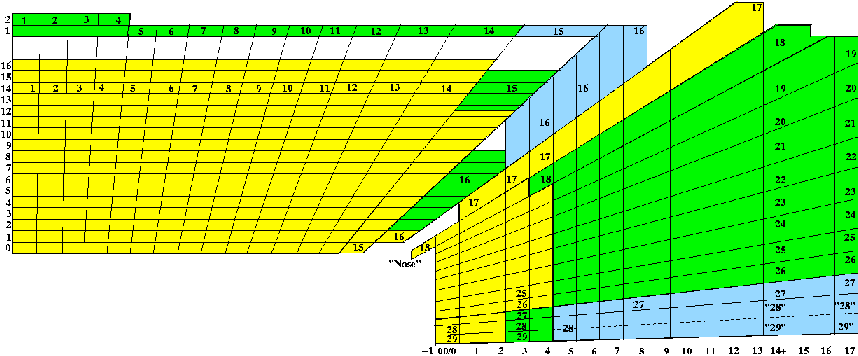
\includegraphics[width=1\textwidth]{pictures/HCAL.pdf}

	\caption[Hadronic calorimeter of CMS]{Schematic view of the towers assembly in barrel and endcap in the r-z plane of the \gls{HCAL}, taken from \cite{CMS2}}
	\label{fig:fig_2_9}
\end{figure}

\subsection*{Magnet}

The superconducting coil is made of niobium-titan alloy, which has a inner diameter of 6.22 m and a length of 13.48. The coil is enclosed in an iron yokes, which gives rise to a magnetic field of 4 Tesla. The barrel part of the iron yoke is 11 long and divided into five rings with a distance of 2.5 along the beam axis, and has a material weight of 6000 tonnes. The end cap of the iron jokes is made of three disk at each side of the detector with a weight of 4600 tonnes.

\subsection*{Muon chambers}

The most outer detector component is the muon detector, which is embedded in the iron yoke. The muon system itself relies for the muon detection on three types of gaseous detectors, the drift tubes, the cathode strip chambers and the resistive plate chambers. In the barrel region, covering the region $|$\gls{eta}$|$ $< 1.2$, 250 drift tube chambers organized in four layers with a distance to the beam pipe of 4-7 meters are installed. To the drift tubes 1 or 2 resistive plates chamber are coupled depending on the layer. The endcap region of the system, covering the region of $|$\gls{eta}$|$ $< 2.4$, 468 cathode strip chambers are installed in both sides of the detector, which are assembled in 4 rings. In the region of $|$\gls{eta}$|$ $< 1.6$  resistive plates chamber are coupled to the cathode strip chambers. Figure \ref{fig:fig_2_10} shows a overview of the muon system.

\begin{figure}[ht]
	\centering
	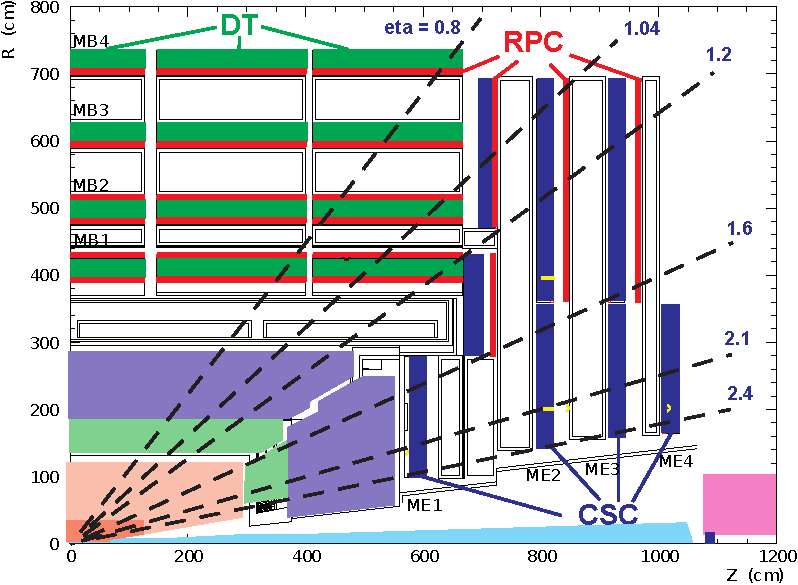
\includegraphics[width=1\textwidth]{pictures/MUON_SYSTEM.pdf}

	\caption[Muon detector system of CMS]{Schematic view of the muon detector system of the r-z plane, where the drift tubes are drawn in green, the resistive plates chamber are drawn in red and the cathode strip chambers are drawn in blue. Taken from \cite{CMS2}}
	\label{fig:fig_2_10}
\end{figure}


\subsection{Trigger system of \gls{CMS}}
\label{sec:section_2_2_3}

The collision rate at the collision point of \gls{CMS} is about 40 Gigahertz, coming from the 25 ns time between the beam bunches, see section \ref{sec:section_2_1_1}. This collision rate at the luminosity of $\mathcal{L} = 10^{34}$ cm$^{-2}$s$^{-1}$  leads to interactions $10^9$ per second. Because the bare amount of data originating from this collisions can neither processed nor saved. Therefore an online selection is done by the \gls{CMS} trigger system \cite{CMS2, TRIGGER}. \\

The first trigger stage is the L1 trigger. This decision of this trigger is taken from the information various local trigger from the detector subsystem, which uses all information recorded of by the calorimeters and the muon system in an event. The second stage is the High Level Trigger \gls{HLT}. Based on the events passing the L1 trigger, the \gls{HLT} decide to keep events on behalf of kinematic variables, which are reconstructed online before the trigger decision. 

\subsection{Particle identification}
\label{sec:section_2_2_4}

The detector components described in the previous section are designed to detect and measure different properties of the particles. Charged particles, like leptons and charged hadrons, have bended trajectories in the magnetic field of \gls{CMS} and leaving hits in the pixel and strip detectors of the tracker system. Neutral particles like photons and neutral hadrons don't leave any track in the tracker system and have a straight trajectory. In the \gls{ECAL} electrons and photons interact with the \gls{PbWO4} and trigger an electromagnetic shower, until the complete energy is deposited. In the \gls{HCAL} all kind of hadrons interact with the brass plates, leading to a cascade of hadron production, until the complete energy is deposited. The muons, which penetrate these sub-detectors losing energy usually only by ionization and leave hits in the muon detector system. Neutrinos can not be measured at all and escape the detector undetected. \\

The bundle of particles, which originating from one object, like a quark or gluon, are jets. There are different algorithms to define and reconstruct jets in \gls{CMS}. Mostly, the anti-kt algorithm is used, counting all particles in a cone with \gls{dR} $= \sqrt{(\Delta \phi)^{2} + (\Delta \eta)^{2}}$.\\ 

From the bending radius of the particles tracks measured in the tracker and for the muons in the muon detector, the transverse momentum \gls{pT} $= \sqrt{p_{x}^{2} + p_{y}^{2}}$ can be measured using 

\begin{equation}
	\label{eq:eq_2_5}
	p_{T} = q\cdot B \cdot R
\end{equation} 

with $q$ as the electric charge of the particle, $B$ the magnetic field flux and R the bending radius of the trajectory. The energy of electrons, photons and hadrons is measured using the energy deposition in the calorimeters. Due to neutrinos and possible \gls{BSM} weakly interacting particles, some energy is not detected. This missing energy measured in the transverse plane (\gls{MET}) is calculated using the fact that in the transverse plane the sum of the momenta of all particles should be zero, due to the protons only having momenta in z-direction. This leads to the formula for \gls{MET}

\begin{equation}
	\label{eq:eq_2_6}
	\vec{E}_{T}^{\text{miss}} = - \sum_{i \in (1, .., n_{\text{meas.}})} \vec{p}_{T}^{i}.
\end{equation}

From the energy and momentum of the visible measured particles, the invariant visible mass distribution \gls{m_vis} of the mother particles can be reconstructed with 

\begin{equation}
	\label{eq:eq_2_6}
	m_{vis} = \sqrt{(E_{1} + E_{2})^2 - (\vec{p}_{1} + \vec{p}_{2})^2}.
\end{equation}


Particles with a short life time, as the $\tau$ lepton, decay into stable particles, which origin from a secondary vertex. To characterize the properties of the particles coming from secondary vertices, the trajectory is extrapolated beyond the secondary vertex and the point of closest approach $d_{0}$ is measured of this extrapolated trajectory and the collision point, see figure \ref{fig:fig_2_11}.

\begin{figure}[ht]
	\centering
	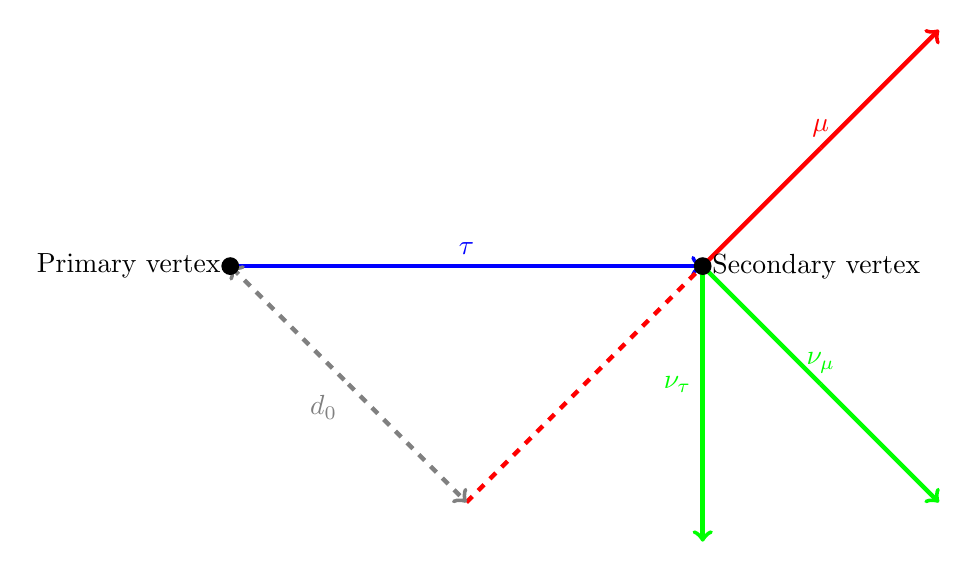
\begin{tikzpicture}
		\draw[blue, ultra thick] (-6,0) -- (-3,0) node[anchor=south] {$\tau$};
		\draw[->, blue, ultra thick] (-6,0) -- (0,0);
		\draw[red, ultra thick] (0,0) -- (1.5,1.5) node[anchor=south] {$\mu$};
		\draw[->, red, ultra thick] (1.5,1.5) -- (3,3);
		\draw[green, ultra thick] (0,0) -- (1.5,-1.5) node[anchor=south] {$\nu_{\mu}$};
		\draw[->, green, ultra thick] (1.5,-1.5) -- (3,-3);
		\draw[green, ultra thick] (0,0) -- (0,-1.5) node[anchor=east] {$\nu_{\tau}$};
		\draw[->, green, ultra thick] (0,-1.5) -- (0,-3.5);
		\draw[red, ultra thick, dashed] (-3,-3) -- (0,0);
		\draw[<-, gray, ultra thick, dashed] (-6,0) -- (-4.5,-1.5) node[anchor=north east] {$d_0$};
		\draw[->, gray, ultra thick, dashed] (-4.5,-1.5) -- (-3,-3);
		\filldraw[black] (-6,0) circle (3pt) node[anchor=east] {Primary vertex};
		\filldraw[black] (0,0) circle (3pt) node[anchor=west] {Secondary vertex};
	\end{tikzpicture}
	\caption[Construction of point of closest approach]{Construction for measuring the point of closest approach $d_{0}$ of the muon trajectory to the collision point}
	\label{fig:fig_2_11}
\end{figure}



\clearpage{\pagestyle{empty}\cleardoublepage}

\chapter{Analysis strategy}
The goal of the analysis is to search for a direct indication of \gls{LFV} in the decay of Z bosons using data from proton-proton collisions measured at \gls{CMS}. Two kinds of process have to be analyzed. The first process is the signal process of the \gls{LFV} decaying Z boson. The second process are background processes of the \gls{SM} leaving the same final state particles as the signal process. To study the differences of signal and background, both are simulated using Monte Carlo simulations (\gls{MC}). Including statistical and systematic uncertainties arising from the measurement, statistical methods are used to evaluate the simulation in comparison to data. 


\section{Signal and background processes}

\subsection{Signal process}
\label{sec:section_3_1_1}

To violate lepton flavour, the individual sum of each lepton flavour in initial and final state must be different: 

\begin{equation}
	\label{eq:eq_3_1}
	\sum_{n \text{ initial state particle}} f_{n} \neq  \sum_{n \text{ final state particle}} f_{n}
\end{equation}

In the case of a Z boson, produced via quark annihilation in a proton proton collider, three possible configurations fulfil the condition. The direct decay of a Z boson into an electron and a muon, referred to as $e\mu$ final state, into an electron and a $\tau$ lepton, referred to as $e\tau$ final state, or into a muon and a $\tau$ lepton, referred to as $\mu\tau$ final state, violates lepton flavour. The feynman diagrams of these processes are shown in figure \ref{fig:fig_3_1}. \\

\begin{figure}[htp]
	\centering

	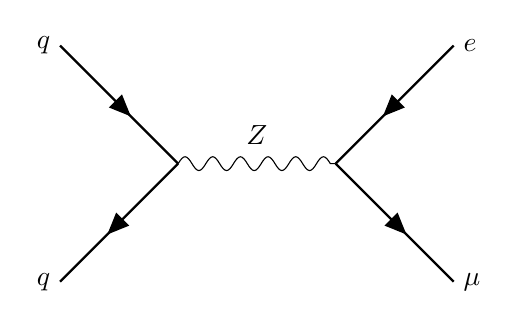
\begin{tikzpicture}[node distance=1.5cm]
		\coordinate[label=left:$q$] (q1);
		\coordinate[below=3cm of q1, label=left:$q$] (q2);
   
		\coordinate[below =1.5cm of q1] (k1); \coordinate[right =1.5cm of k1] (v1); 
		\coordinate[right =2cm of v1] (v2); \coordinate[right =1.5cm of v2] (k2);
		
		\coordinate[above=1.5 cm of k2,label=right:$e$] (l1);
		\coordinate[below=3cm of l1, label=right:$\mu$] (l2);

		\draw[fermion] (q1) -- (v1);
		\draw[fermion] (v1) -- (q2);
		\draw[photon] (v1) -- node[label=above:$Z$] {} (v2);
		\draw[fermion] (l1) -- (v2);
		\draw[fermion] (v2) -- (l2);
	\end{tikzpicture}

	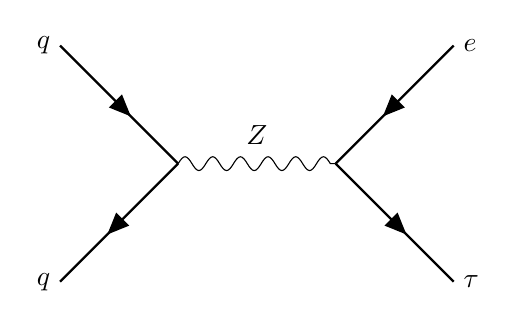
\begin{tikzpicture}[node distance=1.5cm]
		\coordinate[label=left:$q$] (q1);
		\coordinate[below=3cm of q1, label=left:$q$] (q2);
   
		\coordinate[below =1.5cm of q1] (k1); \coordinate[right =1.5cm of k1] (v1); 
		\coordinate[right =2cm of v1] (v2); \coordinate[right =1.5cm of v2] (k2);
		
		\coordinate[above=1.5 cm of k2,label=right:$e$] (l1);
		\coordinate[below=3cm of l1, label=right:$\tau$] (l2);

		\draw[fermion] (q1) -- (v1);
		\draw[fermion] (v1) -- (q2);
		\draw[photon] (v1) -- node[label=above:$Z$] {} (v2);
		\draw[fermion] (l1) -- (v2);
		\draw[fermion] (v2) -- (l2);
	\end{tikzpicture}

	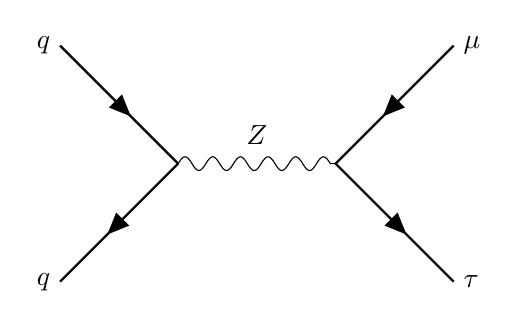
\begin{tikzpicture}[node distance=1.5cm]
		\coordinate[label=left:$q$] (q1);
		\coordinate[below=3cm of q1, label=left:$q$] (q2);
   
		\coordinate[below =1.5cm of q1] (k1); \coordinate[right =1.5cm of k1] (v1); 
		\coordinate[right =2cm of v1] (v2); \coordinate[right =1.5cm of v2] (k2);
		
		\coordinate[above=1.5 cm of k2,label=right:$\mu$] (l1);
		\coordinate[below=3cm of l1, label=right:$\tau$] (l2);

		\draw[fermion] (q1) -- (v1);
		\draw[fermion] (v1) -- (q2);
		\draw[photon] (v1) -- node[label=above:$Z$] {} (v2);
		\draw[fermion] (l1) -- (v2);
		\draw[fermion] (v2) -- (l2);
	\end{tikzpicture}
	
	\caption[Feynman diagram of LFV Z boson decay]{Feynman diagram of LFV Z boson decay into the $e\mu$, $e\tau$ and $\mu\tau$ final state}
	\label{fig:fig_3_1}

\end{figure}

The $\tau$ lepton \cite{TAU} has a special role in comparison to electrons or muons. Due to the mean life time of 2.9$\cdot 10^{-13}$ seconds the $\tau$ lepton decays after a flight distance of a few micrometers and leaves secondary vertices in the tracker system. The $\tau$ lepton can decay leptonically with a branching ratio of $\text{BR}(\tau \to l\nu_{\tau}\nu_{l}) = 0.34$ or hadronically with a branching ratio of $\text{BR}(\tau \to \nu_{\tau} + \text{hadrons}) = 0.66$. Because of the high branching ratio of the hadronic decaying $\tau$ leptons (\gls{TAUH}), only this type of decay is considered in the content of the analysis. The \gls{TAUH} are reconstructed from jets, which originate from the hadrons of the $\tau$ decay. 

\subsection{Background processes}
\label{sec:section_3_1_2}

Background processes have the same particles in the final state as the \gls{LFV}, but they originate from leptonic/semi-leptonic decays of the mother particles or from misidentification of the particles. This leads to differences in kinematic distributions, different secondary vertices and/or additional particles in the final state beside the two leptons. \\

\subsection*{Drell Yan}

The main irreducible background is the Drell-Yan (\gls{DY}) $Z\to\tau\tau$ process, both $\tau$ leptons decays leptonically into an electron, a muon and four neutrinos, or one $\tau$ lepton decays leptonically into a lepton and the other one decays hadronically with three neutrinos. The leptons from the $\tau$ lepton decays originate from secondary vertices and have different kinematic properties in comparison to the leptons originating from \gls{LFV}. Due to the neutrinos, which carries away the momenta undetected, this process will have in general more \gls{MET} in the event compared to the \gls{LFV} process. Figure \ref{fig:fig_3_2} shows the Feynman diagram of the leptonic decay chain. Besides the $Z\to\tau\tau$ process, the second \gls{DY} process is $Z\to\ell\ell$ with $l \in (e, \mu$), where one of the leptons $\ell$ has a misidentified lepton flavour. In this case the kinematic properties are quite similar to the \gls{LFV} process, because the lepton also originate from the $Z$ boson, and have no secondary vertices or neutrinos. \\


\begin{figure}[htp]
	\centering

	\begin{tikzpicture}[node distance=1.5cm]
		\coordinate[label=left:$q$] (q1);
		\coordinate[below=3cm of q1, label=left:$q$] (q2);

		\coordinate[right =1.5cm of k1] (v1); 
		\coordinate[right =2cm of v1] (v2); \coordinate[right =1.5cm of v2] (k2);
	
		\coordinate[above=1.5 cm of k2] (tau1);
		\coordinate[below=1.5cm of k2] (tau2);
	
		\coordinate[right=1.5 cm of tau1] (k3);
		\coordinate[above=1 cm of k3, ] (W1);
		\coordinate[below=1 cm of k3,label=right:$\nu_{\tau}$] (nu1);
		\coordinate[right=1.5 cm of W1] (k4);
		\coordinate[above=1 cm of k4, label=right:$e$] (l1);
		\coordinate[below=1 cm of k4, label=right:$\nu_{e}$] (nu2);
	
		\coordinate[right=1.5 cm of tau2] (k5);
		\coordinate[above=1 cm of k5,label=right:$\nu_{\tau}$] (nu3);
		\coordinate[below=1 cm of k5] (W2);
		\coordinate[right=1.5 cm of W2] (k6);
		\coordinate[above=1 cm of k6, label=right:$\mu$] (l2);
		\coordinate[below=1 cm of k6,label=right:$\nu_{\mu}$] (nu4);
	
		\draw[fermion] (q1) -- (v1);
		\draw[fermion] (v1) -- (q2);
		\draw[photon] (v1) -- node[label=above:$Z$] {} (v2);
		\draw[fermion] (tau1) -- node[label=above:$\tau$] {} (v2);
		\draw[fermion] (v2) -- node[label=below:$\tau$] {} (tau2);
	
   		\draw[fermion] (nu1) -- (tau1);
   		\draw[photon] (tau1) -- node[label=above:$W$] {} (W1);
   		\draw[fermion] (l1) -- (W1);
   		\draw[fermion] (W1) -- (nu2);
	
   		\draw[photon] (W2) -- node[label=below:$W$] {} (tau2);
   		\draw[fermion] (tau2) -- (nu3);
   		\draw[fermion] (l2) -- (W2);
   		\draw[fermion] (W2) -- (nu4);
	\end{tikzpicture}
	
	\caption[Feynman diagram of $Z\to\tau\tau$ decay]{Feynman diagram of $Z\to\tau\tau$ fully leptonic decay in the $e\mu$ final state}
	\label{fig:fig_3_2}
\end{figure}

\subsection*{Top/anti-top production}

One of the other backgrounds is the top/anti-top production (\gls{TTBAR}), in which the top pair decays leptoncally into leptons, b-quarks and neutrinos. Figure \ref{fig:fig_3_3} shows the Feynman diagram of the leptonic decay chain. Like in the $Z\to\tau\tau$ process the leptons originate from secondary vertices and have different kinematic properties in comparison to the signal. \\


\begin{figure}[htp]
	\centering

	\begin{tikzpicture}[node distance=1.5cm]
		\coordinate[label=left:$g$] (g1);
		\coordinate[below=3cm of g1, label=left:$g$] (g2);

		\coordinate[right =1.5cm of k1] (v1); 
		\coordinate[right =2cm of v1] (v2); \coordinate[right =1.5cm of v2] (k2);
	
		\coordinate[above=1.5 cm of k2] (top1);
		\coordinate[below=1.5cm of k2] (top2);
	
		\coordinate[right=1.5 cm of tau1] (k3);
		\coordinate[above=1 cm of k3, ] (W1);
		\coordinate[below=1 cm of k3,label=right:$b$] (b1);
		\coordinate[right=1.5 cm of W1] (k4);
		\coordinate[above=1 cm of k4, label=right:$\ell$] (l1);
		\coordinate[below=1 cm of k4, label=right:$\nu_{\ell}$] (nu1);
	
		\coordinate[right=1.5 cm of tau2] (k5);
		\coordinate[above=1 cm of k5,label=right:$b$] (b2);
		\coordinate[below=1 cm of k5] (W2);
		\coordinate[right=1.5 cm of W2] (k6);
		\coordinate[above=1 cm of k6, label=right:$\ell'$] (l2);
		\coordinate[below=1 cm of k6,label=right:$\nu_{\ell'}$] (nu2);
	
		\draw[gluon] (g1) -- (v1);
		\draw[gluon] (v1) -- (g2);
		\draw[gluon] (v1) -- node[label=above:$g$] {} (v2);
		\draw[fermion] (top1) -- node[label=above:$t$] {} (v2);
		\draw[fermion] (v2) -- node[label=below:$t$] {} (top2);
	
   		\draw[fermion] (b1) -- (top1);
   		\draw[photon] (top1) -- node[label=above:$W$] {} (W1);
   		\draw[fermion] (l1) -- (W1);
   		\draw[fermion] (W1) -- (nu1);
	
   		\draw[photon] (W2) -- node[label=below:$W$] {} (top2);
   		\draw[fermion] (top2) -- (b2);
   		\draw[fermion] (l2) -- (W2);
   		\draw[fermion] (W2) -- (nu2);
	\end{tikzpicture}

	\caption[Feynman diagram of \gls{TTBAR} decay]{Feynman diagram of \gls{TTBAR} decay chain}
	\label{fig:fig_3_3}
\end{figure}

\subsection*{Di-boson}

Besides the decay of fermions like the $\tau$ leptons and the tops, also the lepton decay of a pair of vector bosons leaves to leptons. The possible vector bosons pairs are $ZZ$/$WW$/$WZ$. Figure \ref{fig:fig_3_4} shows the Feynman diagram of vector boson production. For the $WW$ pair, the $W$ bosons decay into two leptons with two neutrinos, for the $ZZ$ pair the Z bosons decay into four leptons, where two leptons are not identified correctly, and for the $WZ$ pair the bosons decay into three leptons and a neutrino, there one of the leptons is not identified correctly. \\


\begin{figure}[htp]
	\centering
	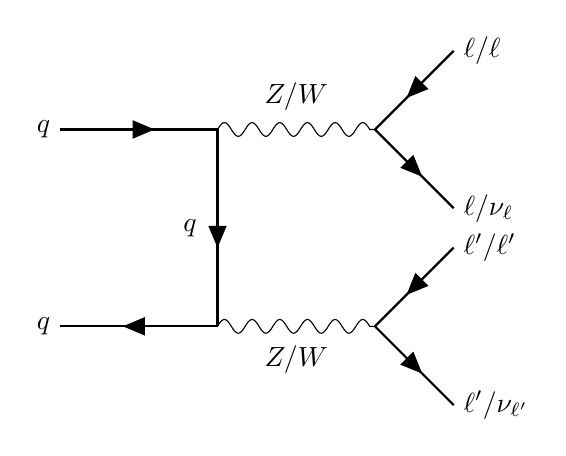
\begin{tikzpicture}[node distance=1.5cm]
		\coordinate[label=left:$q$] (q1);
		\coordinate[right=2cm of q1] (v1);
		\coordinate[below=2.5cm of v1] (v2);
		\coordinate[left=2cm of v2, label=left:$q$] (q2);
		\coordinate[right=2cm of v1] (Z1);
		\coordinate[right=2cm of v2] (Z2);
		
		\coordinate[right=1 cm of Z1] (k1);
		\coordinate[above=1 cm of k1, label=right:$\ell/\ell$] (l1);
		\coordinate[below=1 cm of k1, label=right:$\ell/\nu_{\ell}$] (l2);
		
		\coordinate[right=1 cm of Z2] (k2);
		\coordinate[above=1 cm of k2, label=right:$\ell'/\ell'$] (l3);
		\coordinate[below=1 cm of k2, label=right:$\ell'/\nu_{\ell'}$] (l4);
		
		\draw[fermion] (q1) -- (v1);
		\draw[fermion] (v1)  -- node[label=left:$q$] {} (v2);
		\draw[fermion] (v2) -- (q2);
		\draw[photon] (v1)  -- node[label=above:$Z/W$] {} (Z1);
		\draw[photon] (v2)  -- node[label=below:$Z/W$] {} (Z2);
		
		\draw[fermion] (l1) -- (Z1);
		\draw[fermion] (Z1) -- (l2);
		\draw[fermion] (l3) -- (Z2);
		\draw[fermion] (Z2) -- (l4);
	\end{tikzpicture}

	\caption[Feynman diagram of vector boson process]{Feynman diagram of vector boson process}
	\label{fig:fig_3_4}
\end{figure}

\subsection*{W + jets and \gls{QCD}}

On the other hand processes exist, in which the end state particles are not identified correctly, like discussed for the $Z\to\ell\ell$ process. One of the processes is the single $W$ boson production in association with a quark, as seen in figure \ref{fig:fig_3_5}. The $W$ boson decays leptonically, but the quark jet is misidentified as a lepton or a \gls{TAUH}. The other process are \gls{QCD} multijet processes, which are the result of the hard interaction of the partons from the protons. These processes lead to quarks/gluons in the final state, which jets are then misidentified as leptons. Figure  \ref{fig:fig_3_6} shows two possible Feynman diagrams contributing to the \gls{QCD} background. \\

\begin{figure}[htp]
	\centering
	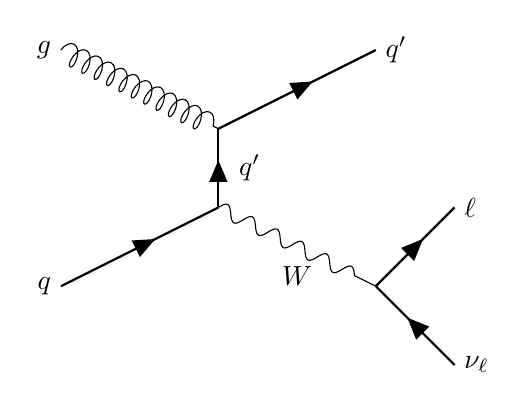
\begin{tikzpicture}[node distance=1.5cm]
		\coordinate[label=left:$g$] (g);
		\coordinate[below=3cm of g, label=left:$q$] (q1);
		
		\coordinate[right=2cm of g] (k);
		\coordinate[below=1cm of k] (v1);
		\coordinate[below=1cm of v1] (v2);
		
		\coordinate[right=4cm of g, label=right:$q'$] (q3);
		\coordinate[right=4cm of q1] (W);

		\coordinate[right=1cm of W] (k2);
		\coordinate[above=1cm of k2, label=right:$\ell$] (l);
		\coordinate[below=1cm of k2, label=right:$\nu_{\ell}$] (nu);
		
		\draw[gluon] (g) -- (v1);
		\draw[fermion] (q1) -- (v2);
		\draw[fermion] (v2) -- node[label=right:$q'$] {} (v1);
		\draw[fermion] (v1) -- (q3);
		\draw[photon] (v2) -- node[label=below:$W$] {} (W);

		\draw[fermion] (nu) -- (W);
		\draw[fermion] (W) -- (l); 
	\end{tikzpicture}

	\caption[Feynman diagram of $W + \text{jets}$ process]{Feynman diagram of $W + \text{jets}$ process}
	\label{fig:fig_3_5}
\end{figure}

\begin{figure}[htp]
		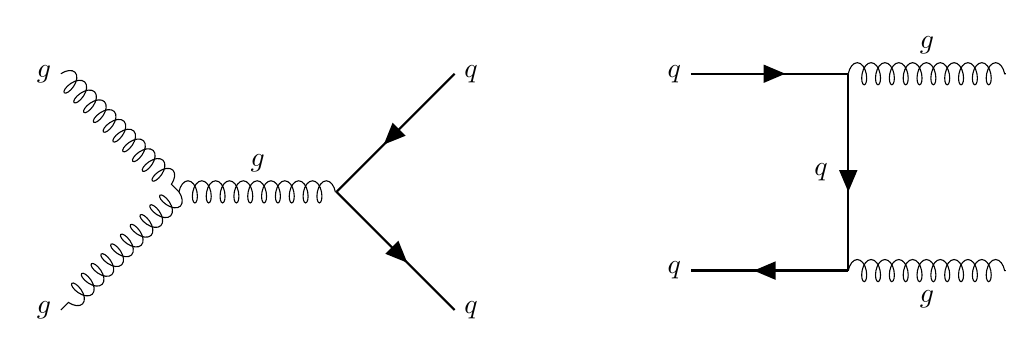
\begin{tikzpicture}[node distance=1.5cm]
			\coordinate[label=left:$g$] (g1);
			\coordinate[below=3cm of g1, label=left:$g$] (g2);   			
			\coordinate[below =1.5cm of g1] (k1); \coordinate[right =1.5cm of k1] (v1); 
			\coordinate[right =2cm of v1] (v2); \coordinate[right =1.5cm of v2] (k2);
		
			\coordinate[above=1.5 cm of k2,label=right:$q$] (q1);
			\coordinate[below=3cm of q1, label=right:$q$] (q2);
	
			\draw[gluon] (g1) -- (v1);
			\draw[gluon] (v1) -- (g2);
			\draw[gluon] (v1) -- node[label=above:$g$] {} (v2);
			\draw[fermion] (q1) -- (v2);
			\draw[fermion] (v2) -- (q2);

			\coordinate[right=3cm of q1, label=left:$q$] (2_q1);
			\coordinate[right=2cm of 2_q1] (2_v1);
			\coordinate[below=2.5cm of 2_v1] (2_v2);
			\coordinate[left=2cm of 2_v2, label=left:$q$] (2_q2);
			\coordinate[right=2cm of 2_v1] (2_g1);
			\coordinate[right=2cm of 2_v2] (2_g2);

			
			\draw[fermion] (2_q1) -- (2_v1);
			\draw[fermion] (2_v1)  -- node[label=left:$q$] {} (2_v2);
			\draw[fermion] (2_v2) -- (2_q2);
			\draw[gluon] (2_v1)  -- node[label=above:$g$] {} (2_g1);
			\draw[gluon] (2_v2)  -- node[label=below:$g$] {} (2_g2);
		\end{tikzpicture}

	
	\caption[Feynman diagram of \gls{QCD} background]{Feynman diagram of two possible contributions to the \gls{QCD} multijet background}
	\label{fig:fig_3_6}
\end{figure}


\section{Event selection}
\label{sec:section_3_2}

From all events, which are recorded by \gls{CMS}, only a fraction of them are particularly interesting regarding the search for \gls{LFV}. The search for \gls{LFV} requires events having leptons with different flavour, which are well reconstructed and isolated. Because of this, an analysis specific event selection is performed. This selection is divided into two steps. The first step is the reconstruction/identification of the objects, where the raw detector information is evaluated with specific software tools. The second step is to select the reconstructed objects of interest in specific events and to set criteria in regard to the quality of reconstruction. 


\subsection{Event reconstruction}
\label{sec:section_3_2_1}

Like discussed in section \ref{sec:section_2_2_4} and illustrated in figure \ref{fig:fig_2_5}, different particles leave specific signatures in the detector systems of \gls{CMS}. This fact is used in the particle flow algorithm (\gls{PF}) \cite{PF}. The algorithm identifies objects electrons and photon from \gls{ECAL} entries or muons from hits in the muon chambers. By linking the information of the different detector systems, for example a track in the tracker system and matching \gls{ECAL} entries, all particles can be identified one after another.  From the combination of all reconstructed particle higher level objects like jets or \gls{MET} are reconstructed. \\

To ensure the best possible identification efficiency of the reconstructed particles, the \gls{CMS} collaboration provides multivariate analysis (\gls{MVA}) classifiers for the different particles. The classifiers are trained to identify the particle of interest from other particles, where information of detector systems are fed into the training, see reference \cite{ERECO} for the electron \gls{MVA} classifier. \\

The $\tau$ leptons require more sophisticated methods for reconstruction, because of the short lifetime and the decay products of the $\tau$ lepton. The \gls{TAUH} are reconstructed with the hadron-plus-strips algorithm \cite{TAURECO}. This algorithm uses information of the tracks and calorimeter deposition of the hadrons originating from the decay of the $\tau$ lepton to a charged pion (1-prong), to a charged pion and a neutral pion (1-prong + $\pi^0$) and to three charged pions (3-prong). \\

As for other objects the \gls{CMS} collaboration provides \gls{MVA} classifier for \gls{TAUH} \cite{TAURECO}. But due to reconstruction of the \gls{TAUH} from decay products, it is more prone that other objects (in general electrons/muons/jets) are misidentified as \gls{TAUH}. For this reason three different \gls{MVA} are provided to differentiate \gls{TAUH} and electrons/muons/jets. \\

Besides $\tau$ leptons, also jets need a sophisticated treatment to be identified from a particle cascade in the calorimeter systems. Jets are reconstructed using the anti-$k_T$ algorithm \cite{ANTIKT}, which cluster all \gls{PF} candidates originating from the primary vertex within a cone of \gls{dR} = 0.4. In this analysis jets are required to fulfil \gls{pT} $> 30$ GeV and $|$\gls{eta}$|$ $ < 4.7$ to be identified as a jet. Due to the \gls{TTBAR} and its decay into b-quarks, the combined secondary vertex algorithm \cite{CSV} is used, which uses information about track-based lifetime information and the secondary vertex to provide a classifier to identify jets from b-quarks. 


\subsection{Selection criteria}
\label{sec:section_3_2_2}

For the search of \gls{LFV} in Z boson decays, events of interest contain a pair of reconstructed electron/muon, electron/tau lepton or muon/tau lepton. On these reconstructed leptons qualitative requirements are set, in order to maximize the confidence in the quality of the reconstruction. \\

The first requirement is the trigger decision of the \gls{HLT}, which is discussed in section \ref{sec:section_2_2_3}. There is not only one trigger decision, but many trigger decisions are made on the objects of interest. The decision of the trigger is based on the \gls{pT} and \gls{eta} of the particles, which are online reconstructed during the trigger decision. 

\begin{description}
	\item [$e\mu$:] In this final state two cross triggers are used, which selects events with one electron and one muon. The first trigger selects an electron with \gls{pT} $> 23$ GeV and $|$\gls{eta}$|$ $< 2.5$ and a muon with \gls{pT} $> 8$ GeV and $|$\gls{eta}$|$ $< 2.4$ and the second trigger requires an electron with \gls{pT} $> 12$ GeV and $|$\gls{eta}$|$ $< 2.5$ and a muon with \gls{pT} $> 23$ GeV and $|$\gls{eta}$|$ $< 2.4$. 
	\item [$e\tau$:] In this final state a single trigger is used to select events with electrons. The trigger requires an electron with \gls{pT} $> 25$ GeV and $|$\gls{eta}$|$ $< 2.1$
	\item [$\mu\tau$:] In this final state a single trigger for selecting events with a muon and a cross trigger for selecting a pair of muon and \gls{TAUH}. The cross trigger requires a muon with \gls{pT} $> 19$ GeV and $|$\gls{eta}$|$ $< 2.1$ and a \gls{TAUH} with \gls{pT} $> 20$ GeV and $|$\gls{eta}$|$ $< 2.5$ and the single trigger requires muons with \gls{pT} $> 22$ GeV and $|$\gls{eta}$|$ $< 2.1$.
\end{description}

The second requirement is the isolation of the leptons. The isolation quantifies the energy deposition around a reconstructed object in a cone defined by a specific value of \gls{dR}. The definition of isolation is given by

\begin{equation}
	\label{eq:eq_3_1}
	I^{\ell} = \frac{\sum_{\text{charged}} p_{T} + \text{max}(0, \sum_{\text{neutral}} p_{T} - \frac{1}{2}\sum_{\text{charged, PU}} p_{T})}{p_T^{\ell}}  
\end{equation} 

with $\sum_{\text{charged}}$ \gls{pT} as sum of the scalar transverse momenta of all charged particles originating from the primary vertex, $\sum_{\text{neutral}}$ \gls{pT} as sum of the scalar transverse momenta of all neutral particles and $\sum_{\text{charged, PU}}$ \gls{pT} as sum of the scalar transverse momenta of all charged particles from secondary vertices in a cone of \gls{dR} = 0.4. In this analysis tight isolated lepton are required, which means for each final state: 

\begin{description}
	\item [$e\mu$:] For the electron an isolation of $I^{e} \leq  0.15$ and for the muon $I^{\mu} \leq  0.2$ are required. 
	\item [$e\tau$:]  For the electron an isolation of $I^{e} \leq  0.10$ is required. For the \gls{TAUH} a \gls{MVA} ID is used for quantifying isolation, which is trained to distinguish between quark/gluon jets. 
	\item [$\mu\tau$:]  For the muon an isolation of $I^{\mu} \leq 0.10$ is required. Like in the $e\tau$ final state the \gls{TAUH} has to pass the \gls{MVA} ID for isolation.
\end{description}


The third requirement is based on the identification of the particle. To ensure that the object of interest is correctly identified, an offline criteria based on the detectors entries and particles properties are either used to set cuts on this or to train a \gls{MVA} classifier, like mentioned in section \ref{sec:section_3_2_1}. The \gls{CMS} collaboration provides recommendations for each particle, where different so-called working points for the selections are defined. These range from very loose to very tight, where a tighter working indicates a more trustworthy selection, but of course also lead to less events, which are selected. Which working point gives the best balance depends on the analysis, the following list shows the choice for this analysis. 

\begin{description}
	\item [$e\mu$:] The electron has to pass the tight \gls{MVA} identification criteria, while the muon has to pass the medium cut based identification criteria. 
	\item [$e\tau$:]  The electron has to pass the tight \gls{MVA} identification criteria, while the \gls{TAUH} has to pass the tight \gls{MVA} identification criteria to be distinguished from electrons and the loose \gls{MVA} identification criteria to be distinguished from muons.
	\item [$\mu\tau$:]  The muon has to pass the medium cut based identification criteria, while the \gls{TAUH} has to pass the loose \gls{MVA} identification criteria to be distinguished from electrons and the tight \gls{MVA} identification criteria to be distinguished from muons.
\end{description}


\subsection{Categorization}
\label{sec:section_3_2_3}

The events from signal and background processes differ in their kinematics properties. This fact can be used in the statistical interpretation of the analysis, see section \ref{sec:section_5_2}. A categorization of the phase space is applied, which defines different region of interest. \\

In this analysis the number of jets are of interest. As discussed in section \ref{sec:section_3_1_2}, the \gls{LFV} signal leads always to leptons with different flavour. There are two possible sources of jets for signal events. One source are jets, which are radiated from quarks before their annihilation to the Z boson. The other source of jets in the final state are quarks/gluons coming from the other constituents of the proton. The same argumentation is also true for the \gls{DY} background. This leads to a distribution, where most events have zero jets and the number of jets in events is expected to be smaller for each additional jet. In comparison, some background processes have always jets in their final state. Backgrounds like \gls{TTBAR}, W + jets and \gls{QCD} multijet have jets in the final state because of the properties of the interaction or the decay of the final state particles, as discussed in section \ref{sec:section_3_1_2}. The described jet distributions are shown in figure \ref{fig:fig_3_7}. \\

\begin{figure}[htp]
	\centering
	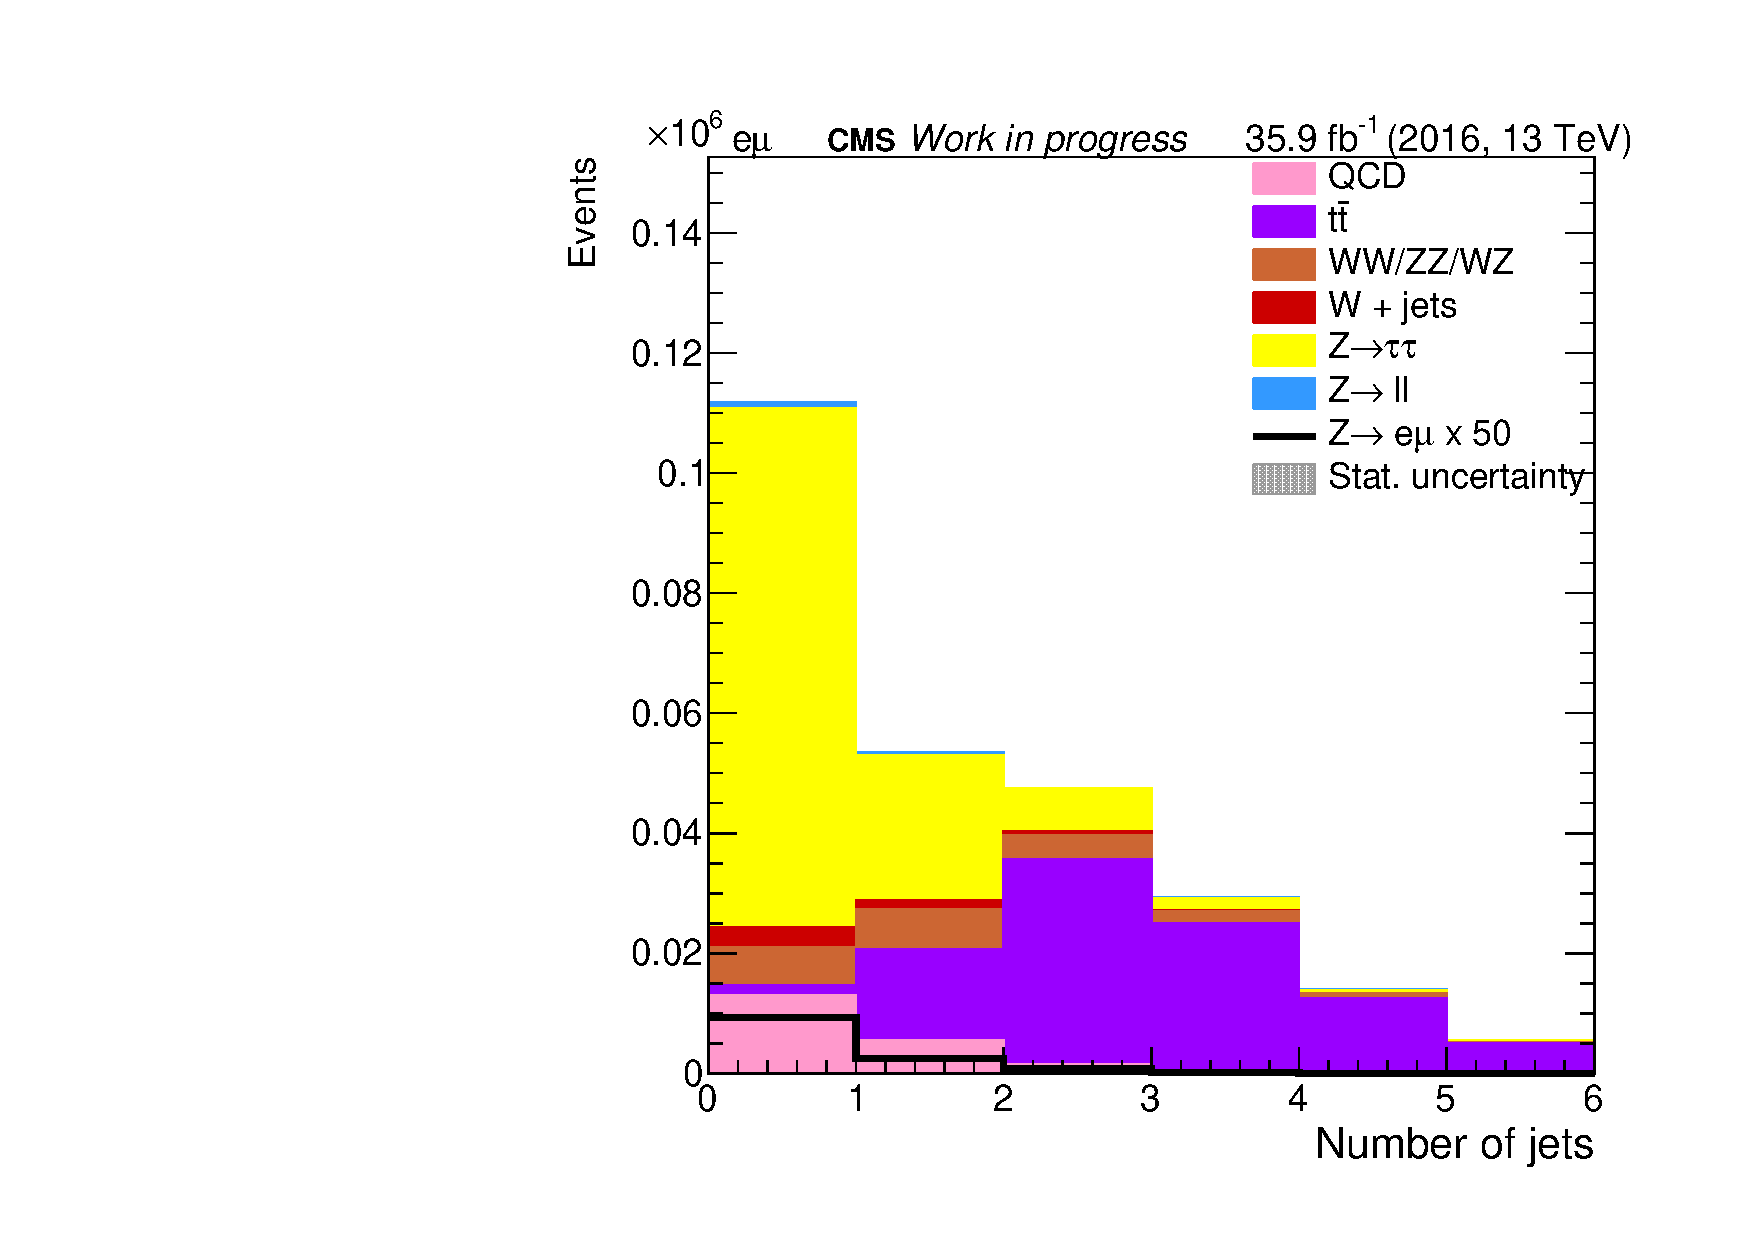
\includegraphics[width=0.55\textwidth]{plots/em/NumberOfJets.pdf}
	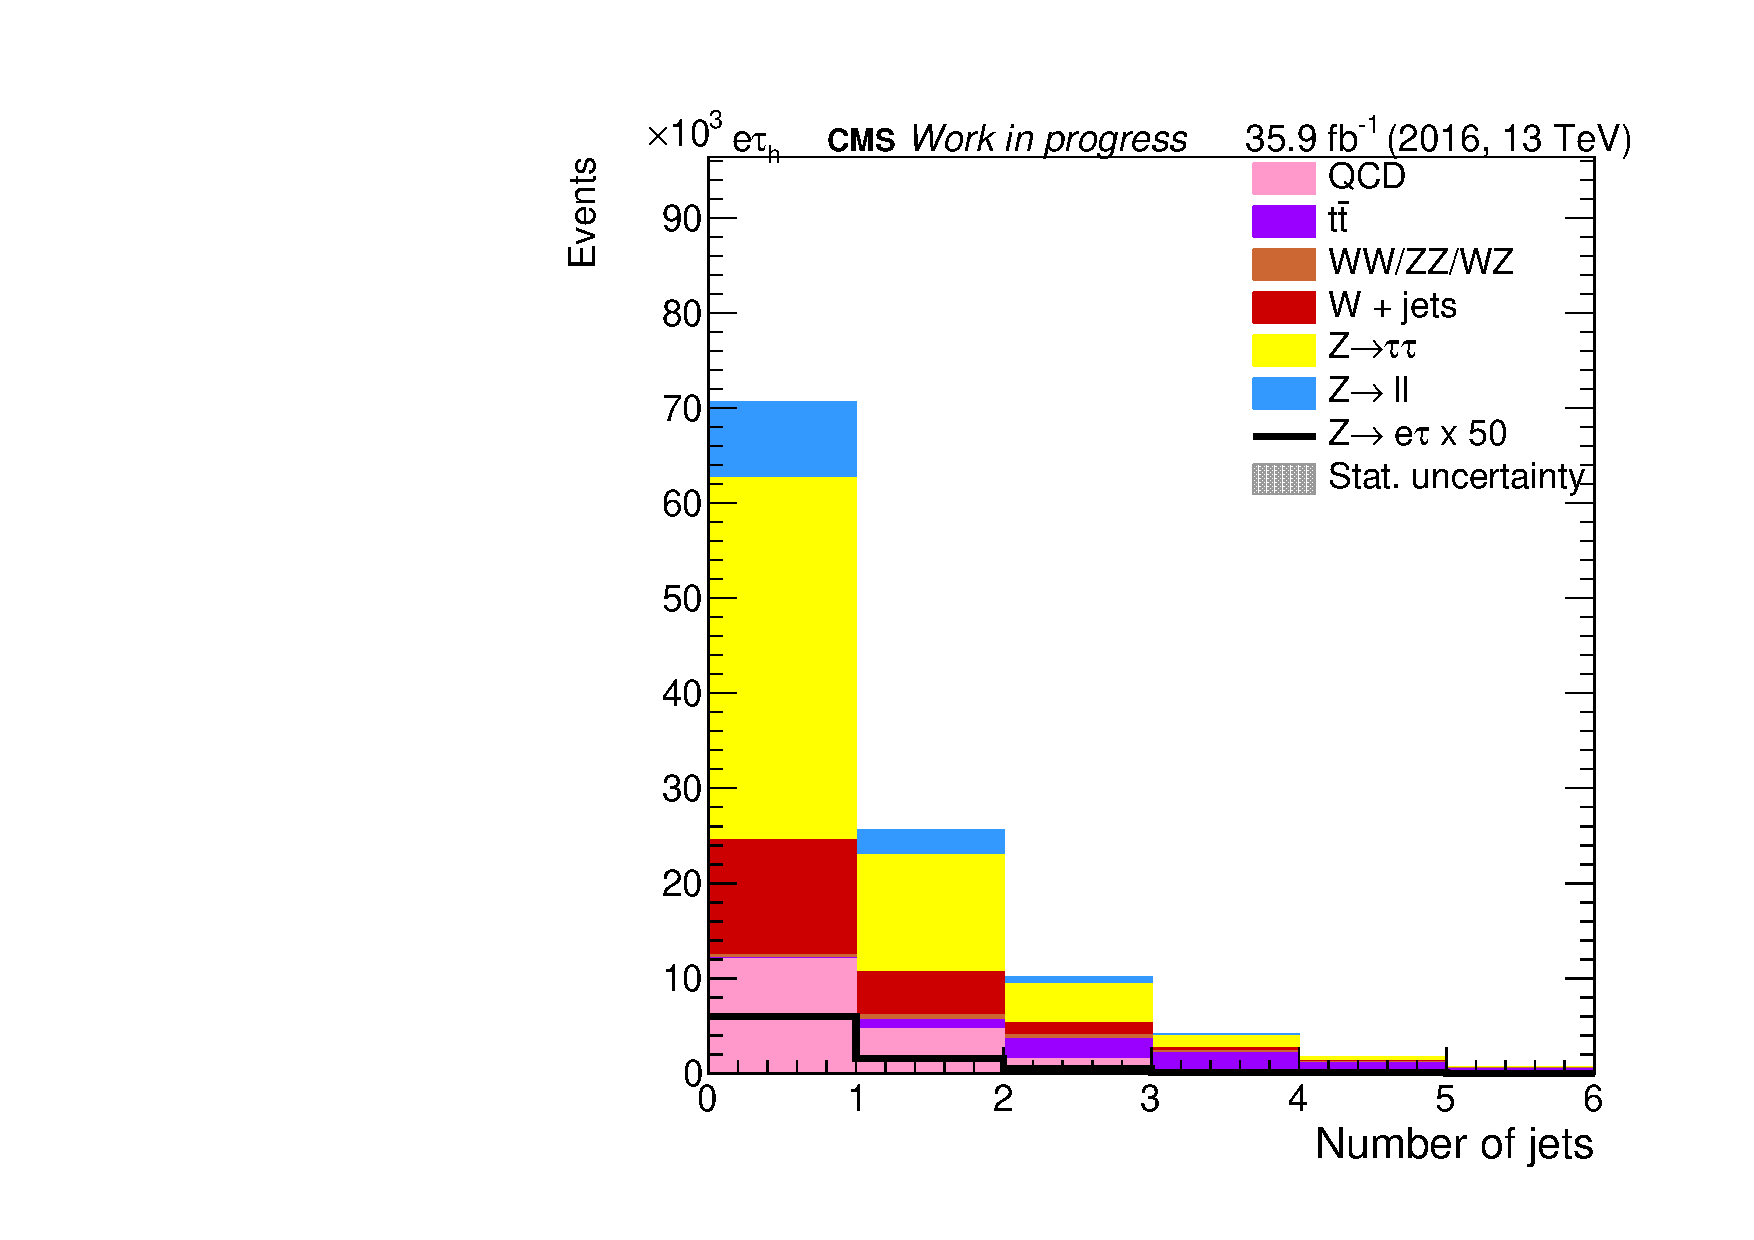
\includegraphics[width=0.55\textwidth]{plots/et/NumberOfJets.pdf}
	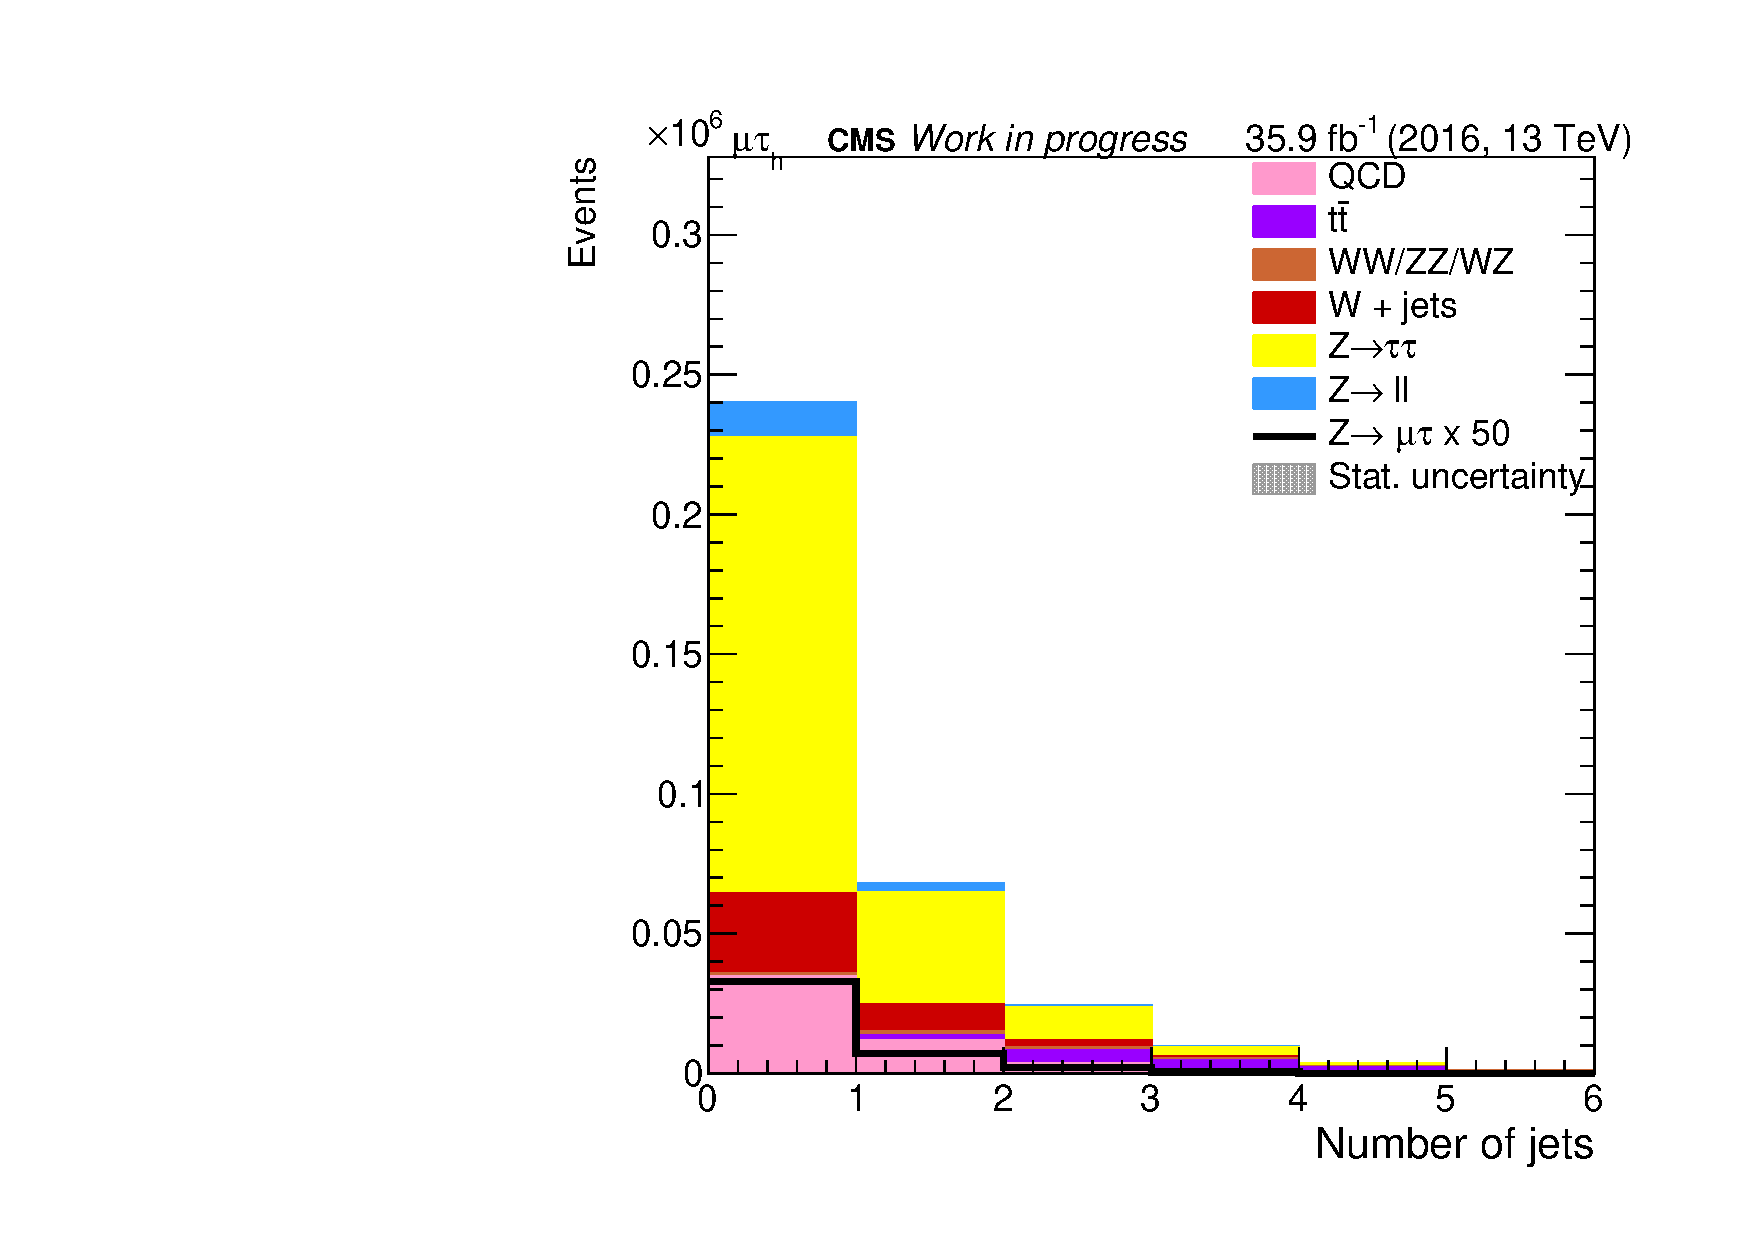
\includegraphics[width=0.55\textwidth]{plots/mt/NumberOfJets.pdf}

	\caption[Number of jet distribution of each final state]{Number of jet distribution for the final state $e\mu$, $e\tau$ and $\mu\tau$}
	\label{fig:fig_3_7}
\end{figure}

For the categorization a cut on the jets multiplicity is applied. Three distinguished regions in phase space are considered:

\begin{description}
	\item [Zero Jet category:] Event with zero jets
	\item [One Jet category:] Event with one jet
	\item [Multi Jet category:] Event with more than one jet
\end{description}


\section{Signal expectation}
\label{sec:section_3_3}

The analysis uses a model independent approach for modelling the signal. This means no theoretical prediction of the branching ratios $\text{BR}(Z\to\text{LFV})$ is given like in the case of \gls{LFV} induced by neutrino oscillation, see section \ref{sec:section_1_3_2}. For this reason the signal expectation is constructed by using information of previous analyses, as discussed in section \ref{sec:section_1_3_3}. The previous analysis set limits on the branching ratios for \gls{LFV} process $\text{BR}(Z\to\text{LFV})$ in each final state, and using this information the signal expectation in this analysis is  set to be

\begin{equation}
	\label{eq:eq_3_3}
	N_{\text{LFV}} = \mathcal{L}_{int} \cdot \sigma(pp\to Z) \cdot \text{BR}(Z\to\text{LFV}), \quad \text{LFV} \in (e\mu, e\tau, \mu\tau)
\end{equation}

with the integrated luminosity $\mathcal{L}_{int}$ and the production cross section for Z bosons at proton-proton collisions $\sigma(pp\to Z)$. Because the $\text{BR}(Z\to\text{LFV})$ is an upper limit for each final state, $N_{\text{LFV}}$ can be interpreted as maximal number of events, which can be expected. \\

The three possible decays of the Z boson into \gls{LFV} are analysed independently, which means that for only the final state of interest a non-vanishing branching ratio is assumed. For example the analysis of the $e\mu$ final state assumes a $\text{BR}(Z\to e\mu) > 0$ and  $\text{BR}(Z\to e\tau) = \text{BR}(Z\to \mu\tau) = 0$. 


\section{Background estimation}

The study of both signal and background processes requires the study of simulations, which can be compared with data. The simulation of the processes are provided by the \gls{CMS} collaboration and are done in three steps. The first is the simulations of the physical process by using a \gls{MC} event generator, for example like Madgraph \cite{MADGRAPH}, which generates mother, daughter particles and their four momenta. The second step is the simulation of proton-proton collisions, including the information of the generated particles. In the last step the detector response of \gls{CMS} is simulated by Geant4 \cite{GEANT4} using the proton-proton and the process simulation. \\

In this simulation the physical expectation for the number of events, given by formula \ref{eq:eq_2_2}, is not included yet. This expectation is determined with the background estimation for each process.

\subsection{Background estimated from Monte Carlo simulation}
\label{sec:section_3_4_1}

To determine background from Z boson decays, \gls{MC} simulation is used and normalized to the cross section and integrated luminosity according to equation \ref{eq:eq_2_2}. It is split into two contributions due to different decay modes of the Z. The first contribution is the $Z\to\tau\tau$ background, where depending on the decay mode of the $\tau$ lepton, \gls{TAUH} are matched to generated hadronic taus and electrons/muons are matched generated leptonic decaying taus. The second contribution is the $Z\to\ell\ell$ background, which combines events where \gls{TAUH} is matched to a generated electron/muon or not matched at all. \\ 

The $t\bar{t}$ and the di-boson background, including all production modes of two vector bosons, top quark in association with a W boson and single top production, is simulated with \gls{MC} and normalized to its cross section and the integrated luminosity. 


\subsection{Background estimated using data driven methods}
\label{sec:section_3_4_2}

For the $e\mu$ final state, $W + \text{jets}$ is a minor background due to the small probability for a jet to be misidentified as an isolated lepton. Because of this, in this final state the estimation is done with \gls{MC} simulation and normalized with cross section and integrated luminosity. The \gls{QCD} shape is taken from a region, where both leptons have the same charge (same-sign region) and pass relaxed isolation criteria. The normalization is extrapolated from comparing same-sign (SS) and opposite-sign (OS) regions, where one of the two leptons fulfil $0.3 < I^{\ell} < 0.5$.  \\

In the case of the $e\tau$ / $\mu\tau$ final state, $W + \text{jets}$ normalization and \gls{QCD} is simultaneously estimated with a data driven method. The number of events in the OS signal region (SR), where events fulfil $M_T < 50$ GeV (low $M_T$), is calculated with 

\begin{equation}
	W^{\text{low } M_T}_{OS} = \Bigg(\frac{W^{\text{low } M_T}_{\text{sim. relaxed OS}}}{W^{\text{high } M_T}_{\text{sim. relaxed OS}}}\Bigg) \cdot W^{\text{high } M_T}_{OS}
\end{equation}

with $W^{\text{low } M_T}_{\text{sim. relaxed OS}}$ and $W^{\text{high } M_T}_{\text{sim. relaxed OS}}$ as number of events taken from simulation, where relaxed isolation criteria is applied. For the number of events in the OS region in the control region (CR), where events fulfil $M_T > 50$GeV (high $M_T$), is extracted from data using 

\begin{equation}
	W^{\text{high } M_T}_{OS} = \text{data}^{\text{high } M_T}_{OS} - Z^{\text{high } M_T}_{OS} - t\bar{t}^{\text{high } M_T}_{OS} - \text{diboson}^{\text{high } M_T}_{OS} - \text{QCD}^{\text{high } M_T}_{OS}
\end{equation}

with data and all other backgrounds explained in the previous section. The number of events for QCD in the high $M_T$ region with OS events are estimated using

\begin{equation}
\text{QCD}^{\text{high } M_T}_{OS} = \epsilon^{QCD}_{OS/SS} \cdot (\text{data}^{\text{high } M_T}_{SS} - Z^{\text{high } M_T}_{SS} - t\bar{t}^{\text{high } M_T}_{SS} - \text{diboson}^{\text{high } M_T}_{SS} - W^{\text{high } M_T}_{\text{sim. SS}})
\end{equation}

with simulated $W + \text{jets}$ events, in the SS high $M_T$ CR region. The factor $\epsilon^{QCD}_{OS/SS}$ is an extrapolation from SS to OS region, which is calculated using samples with inverted isolation criteria of the leptons. Using the same extrapolation factor, the distribution of QCD in the low $M_T$ signal region is calculated using 

\begin{equation}
	\text{QCD}^{\text{low } M_T}_{OS} = \epsilon^{QCD}_{OS/SS} \cdot (\text{data}^{\text{low } M_T}_{SS} - Z^{\text{low } M_T}_{SS} - t\bar{t}^{\text{low } M_T}_{SS} - \text{diboson}^{\text{low } M_T}_{SS} -  \Bigg(\frac{W^{\text{low } M_T}_{\text{OS}}}{W^{\text{high } M_T}_{\text{sim. OS}}}\Bigg) \cdot W^{\text{low } M_T}_{\text{SS}})
\end{equation}


\subsection{Correction of simulated events}
\label{sec:section_3_4_3}

Limited power of modelling the proton-proton-interactions, pile up and the detector response leads to discrepancies between the \gls{MC} simulation and data. To correct such discrepancies, scale factors and kinematic corrections are applied. In general the factors for the corrections are provided by the \gls{CMS} collaboration. \\

Trigger and identification of particles shows different efficiencies in data and \gls{MC}. With scale factors binned in \gls{pT} and \gls{eta}, these efficiencies of \gls{MC} are matched to data. For the identification the scale factors depend on the working point of the identification selection. For the case of the \gls{TAUH}, where extra \gls{MVA} identifications to discriminate electrons and muons are used, scale factors in bins of \gls{eta} are applied. \\

Besides selection efficiencies, corrections on the measured energy/momentum have to be applied. In the case of the \gls{TAUH}, the four momenta is corrected by -1.8\% in the 1-prong decay mode, by +1.0\% in the 1-prong + $\pi^{0}$ decay mode and by 0.4\% in the 3-prong decay mode. To correct the energy scales of electrons/muons faking a \gls{TAUH} the four momentum of \gls{TAUH}, which are matched on generator level to an electron or muon, are corrected. For matched \gls{TAUH} to a muons a correction of -0.2\% for the 1-prong decay mode and of +1.5\% for the 1-prong + $\pi^{0}$ decay mode is applied. For matched \gls{TAUH} to an electron a correction of 9.5\% in the 1-prong + $\pi^{0}$ decay mode is applied. \\

For the jet energy scale factors on the jet four momenta are applied. The \gls{MET} is corrected by a propagating the jet energy corrections through the calculation of the MET. For the Z boson and top quark, \gls{pT} corrections are applied. \\

For the $Z\to\tau\tau$ process, scale factors are calculated from a $Z\to\mu\mu$ control sample, where 2D scale factors in \gls{pT} and \gls{m_vis} are calculated like in the SM $H\to\tau\tau$ analysis \cite{SMHTT}. For the corrections of \gls{TTBAR}, scale factors depending on the generated top \gls{pT} are applied.


\section{Discriminating variable}
\label{sec:section_3_5}

The goal of the analysis is to find a excess in data, which could indicate \gls{LFV}. To find an excess, which is not covered by statistical/systematic uncertainties of the background simulation, a discriminating variable has to be chosen for the analysis, which separates the signal and background processes. In general two approaches can be studied. The first approach is a cut-based strategy, in which a set of sensitive parameters are chosen, then cuts are applied on these parameters to enhance the signal/background ratio, while keeping enough events for a sufficient statistical analysis. The second approach are the usage \gls{MVA} classifier, as already introduced in the identification of leptons in section \ref{sec:section_3_2_2}. The \gls{MVA} classifier is trained on events, where the classification is already known (signal or background), and then is later applied on events with unknown classification. 

\subsection{Boosted decision tree}
\label{sec:section_3_5_1}

A boosted decision tree (\gls{BDT}) \cite{BDT} is a continuous binary \gls{MVA} classifier, which can distinguish between two kind of sets, which can be classified. In the case of this analysis, one set is the collection of all backgrounds, and the second set is the \gls{LFV} signal. For each final state independently, a \gls{BDT} classifier is trained to discriminate between the collection of all backgrounds and the signal. \\

The boosted decision tree is an iteration of the many decision trees (\gls{DT}). Figure \ref{fig:fig_3_10} shows the schematic overview which is explained in the following. A set of $N_{events}$ events, where each event $j$ has a event weight $w_{j}$ and a tuple of parameters $x = (x_{1}, ... , x_{i})$ with $i \in \mathbb{N}$, is given as the input of the \gls{DT}. The events have a known labelling, for example background (B) and signal (S). For the set the signal purity is defined as

\begin{equation}
	\label{eq:eq_3_10}
	P = \frac{\sum_{j \in (\text{signal events})} w^{j}}{\sum_{j \in [1, N_{events}]} w^{j}}.
\end{equation}

From the parameter tuple $x$ the parameter $x_{i}$ and the cut value are chosen, which gives the best separation of the samples, which is quantified for example by the gini index 

\begin{equation}
	\label{eq:eq_3_11}
	g = \sum_{j \in [1, N_{events}]} w^{j} \cdot P \cdot (1-P).
\end{equation}

The set is split into two subsets, one having a higher signal purity, while the other subset is higher background purity. On these subsets the same procedure is followed, until the stop condition is hit (maximal number of iterations, minimal numbers of events in a subset, perfect signal/background separation). The events are labelled by the \gls{DT} according the last subset, they land in. This gives a non-continuous binary classification of each event by the \gls{DT}. \\

\begin{figure}[htp]
	\centering
	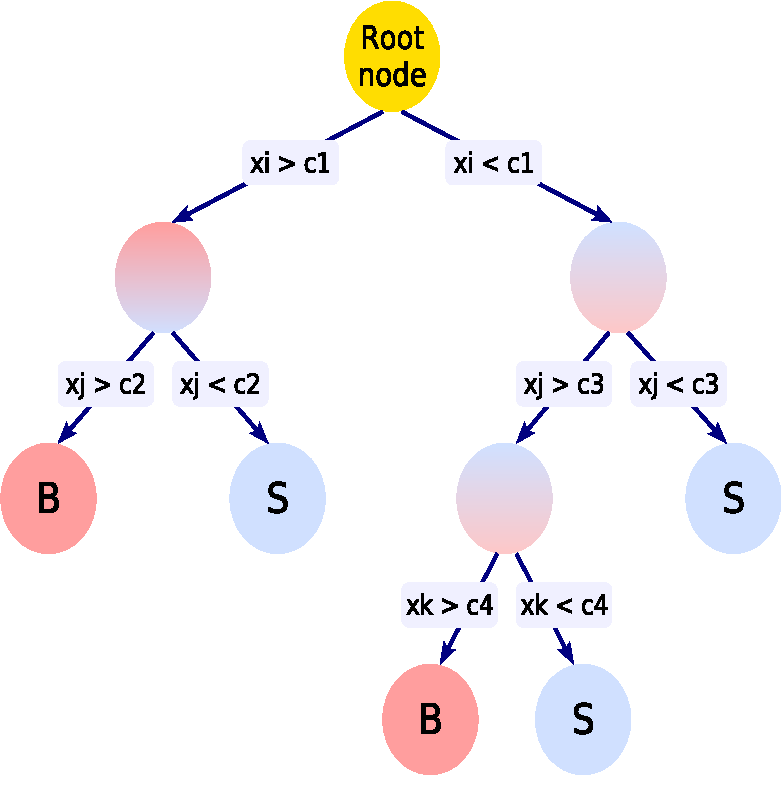
\includegraphics[width=0.7\textwidth]{pictures/DT.pdf}

	\caption[DT scheme]{Scheme of a generic decision tree, taken from \cite{TMVA}}
	\label{fig:fig_3_10}
\end{figure}


In the algorithm of the \gls{BDT} $N_{T}$ \gls{DT} are trained and incorrectly classified events are re-weighted. For each decision tree \gls{DT} $k$ the event $j$ has weight $w^{j}_{k}$. After the $k^{\text{th}}$ \gls{DT} training the misidentification probability is calculated with

\begin{equation}
	\epsilon_{k} = \frac{\sum_{j}^{N_{events}} w^{j} \cdot \text{isMisidentified}(j)}{\sum_{j}^{N_{events}} w^{j}}.
\end{equation}

For the next \gls{DT} all misclassified events are re-weighted with $w^{j}_{k+1} = w^{j}_{k} \cdot e^{\alpha_{k}}$ with $\alpha_{k} = \beta \cdot \ln{\frac{1-\epsilon_{k}}{\epsilon_{k}}}$ and $\beta$ as learning rate, which gives misclassified events a higher impact of decisions of the set splitting. To quantify the result of the iterations of all \gls{DT}, a continuous parameter, the so-called BDT score, is defined as 

\begin{equation}
	\label{eq:eq_3_12}
	T(j) = \frac{1}{\sum_l^{N_T} \alpha_k} \sum_k^{N_T} \alpha_k \cdot T_k(j)
\end{equation}

with $T_k(j)$ as the binary output of the $k^{\text{th}}$  decision tree. The BDT score is constructed in a way, that is ranges from -1 to 1. In case of the analysis, all signal-like events are bigger than zero and all background-like events are smaller than zero. 


\subsection{Training and application}
\label{sec:section_3_5_2}

The \gls{BDT} algorithm explained in section \ref{sec:section_3_5_1} has a set of free tunable parameters, which is called hyperparameter space. The hyperparameters influence the performance of the training and are tuned to give the best separation between background and signal. In this analysis the choice for the hyperparameters are:

\begin{itemize}
	\item Number of decisions trees: 800
	\item Maximal number of iteration in a decision tree: 4
	\item Minimum number of events in a subset: $0.025 \cdot N_{events}$
	\item Learning rate: 0.1
\end{itemize}

The events, on which the training is performed, are taken from the \gls{MC} simulation of all backgrounds and the \gls{LFV} signal that pass the event selection, which is discussed in section \ref{sec:section_3_2_2}. The initial weights are chosen according the physical expectation discussed in the section \ref{sec:section_3_4_1} of the background estimation. For the \gls{QCD} multijet, which is estimated from data driven techniques, no events can be used for the training. Under the assumption, that the \gls{QCD} events in data are labelled as background-like in a \gls{BDT},  the training is performed without \gls{QCD} information. \\

The properties of signal and background processes are reflected in the kinematic distributions of the leptons and the reconstructed Z boson. Because of this, the parameter tuple $x$ includes

\begin{description}
	\item [Angular correlations:] $\Delta \phi(\ell_1, \ell_2)$, $\Delta \phi(\ell_1, {E}_{T})$, $\Delta \phi({E}_{T}, \ell_2)$, $\Delta \phi(\ell_1, Z)$, $\phi(Z, \ell_2)$, $\Delta \theta(\ell_1, \ell_2)$
	\item [Lepton properties:] $p_T(\ell_1)$,  $p_T(\ell_2)$, $|d_0(\ell_1)|$, $|d_0(\ell_2)|$, $m_T(\ell_2)$
	\item [Reconstructed $Z$ boson properties:] $p_T(Z)$, $m_T(Z)$, $E(Z)$, $m_{vis}$, ${E}_{T}$
\end{description}

The plots of all parameter are shown in appendix \ref{sec:appendix_A}. \\

For the training of the \gls{BDT} the TMVA software package \cite{TMVA} is used. The different final state is trained independently from each other. For each final state, two trainings are performed. The training events of the \gls{MC} simulation are split into even-numbered and odd-numbered event sets. The odd-numbered set is used for the training of the \gls{BDT} classifier, and is then applied on the even-numbered set for data and \gls{MC}, and vice versa. This procedure enables the use of the complete \gls{MC} events without statistical biases. 

\subsection{BDT output}
\label{sec:section_3_5_3}

The trained \gls{BDT} assigns the \gls{BDT} score to each event according to formula \ref{eq:eq_3_12}. The \gls{BDT} score is then used as the discriminating variable for the statistical analysis described in section \ref{sec:section_5_1}. Figure \ref{fig:fig_3_11} shows the inclusive distribution of the \gls{BDT} score and a unblinded signal-free \gls{BDT} score distribution each final state. \\

 
\begin{figure}[htp]
	\centering

	\begin{multicols}{2}
		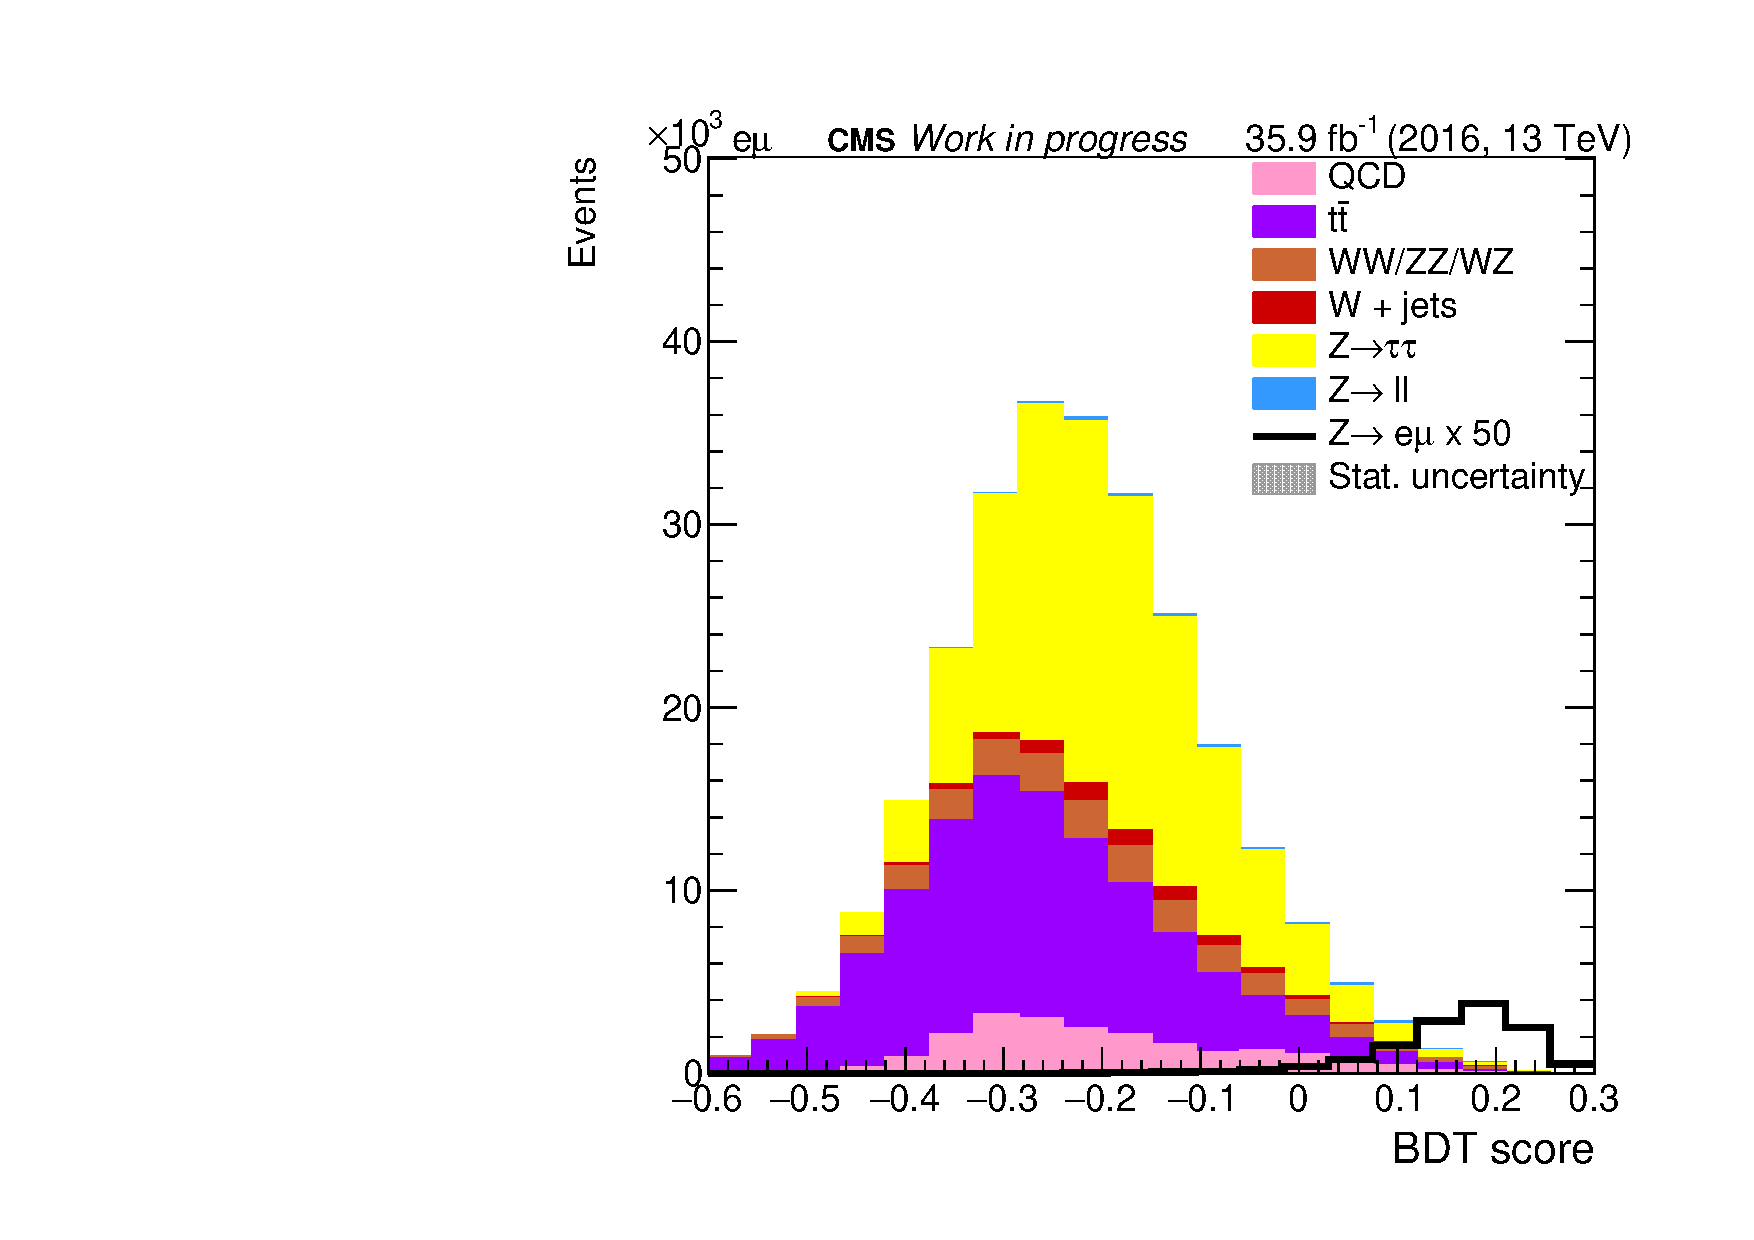
\includegraphics[width=\linewidth]{plots/em/BDTScore.pdf}\par 
		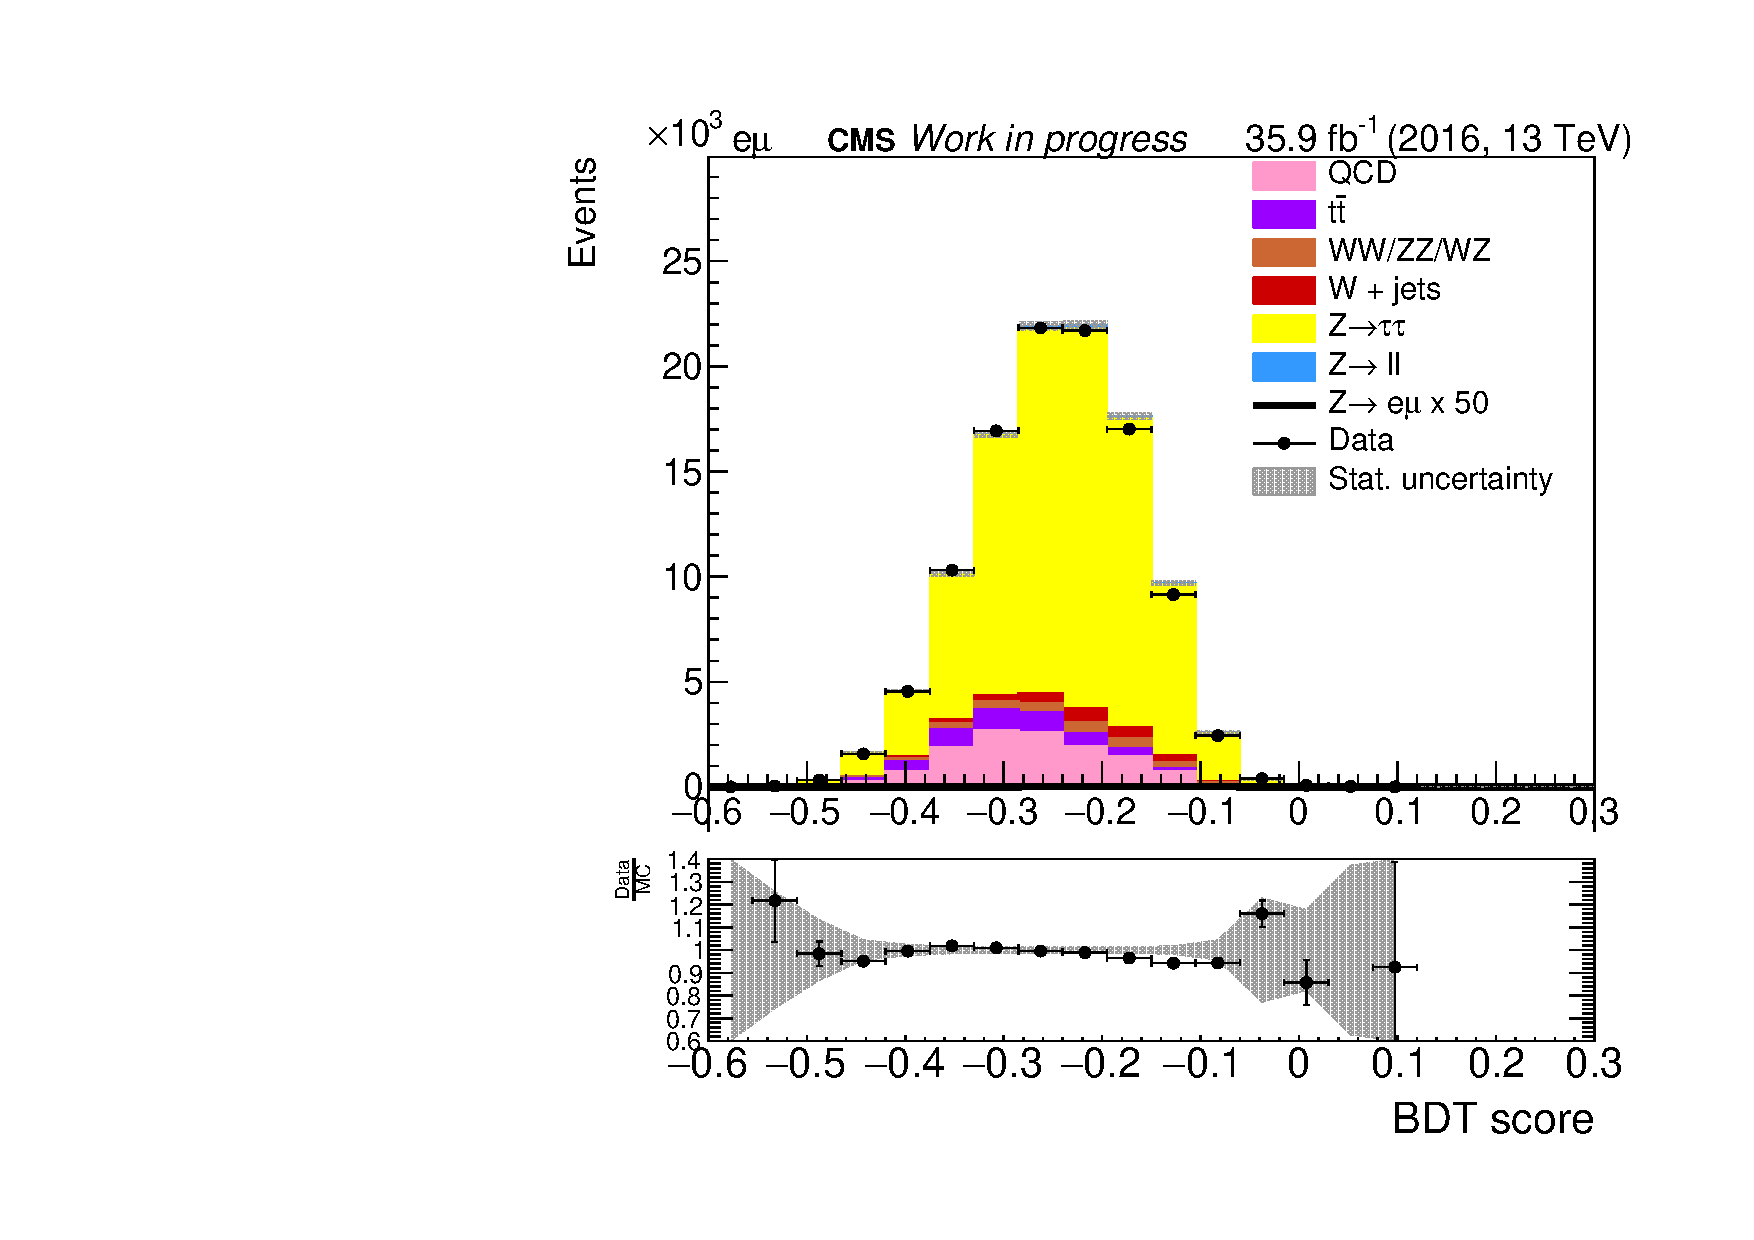
\includegraphics[width=\linewidth]{plots/em/BDTScore_ZTTCR}\par
	\end{multicols}

	\begin{multicols}{2}
		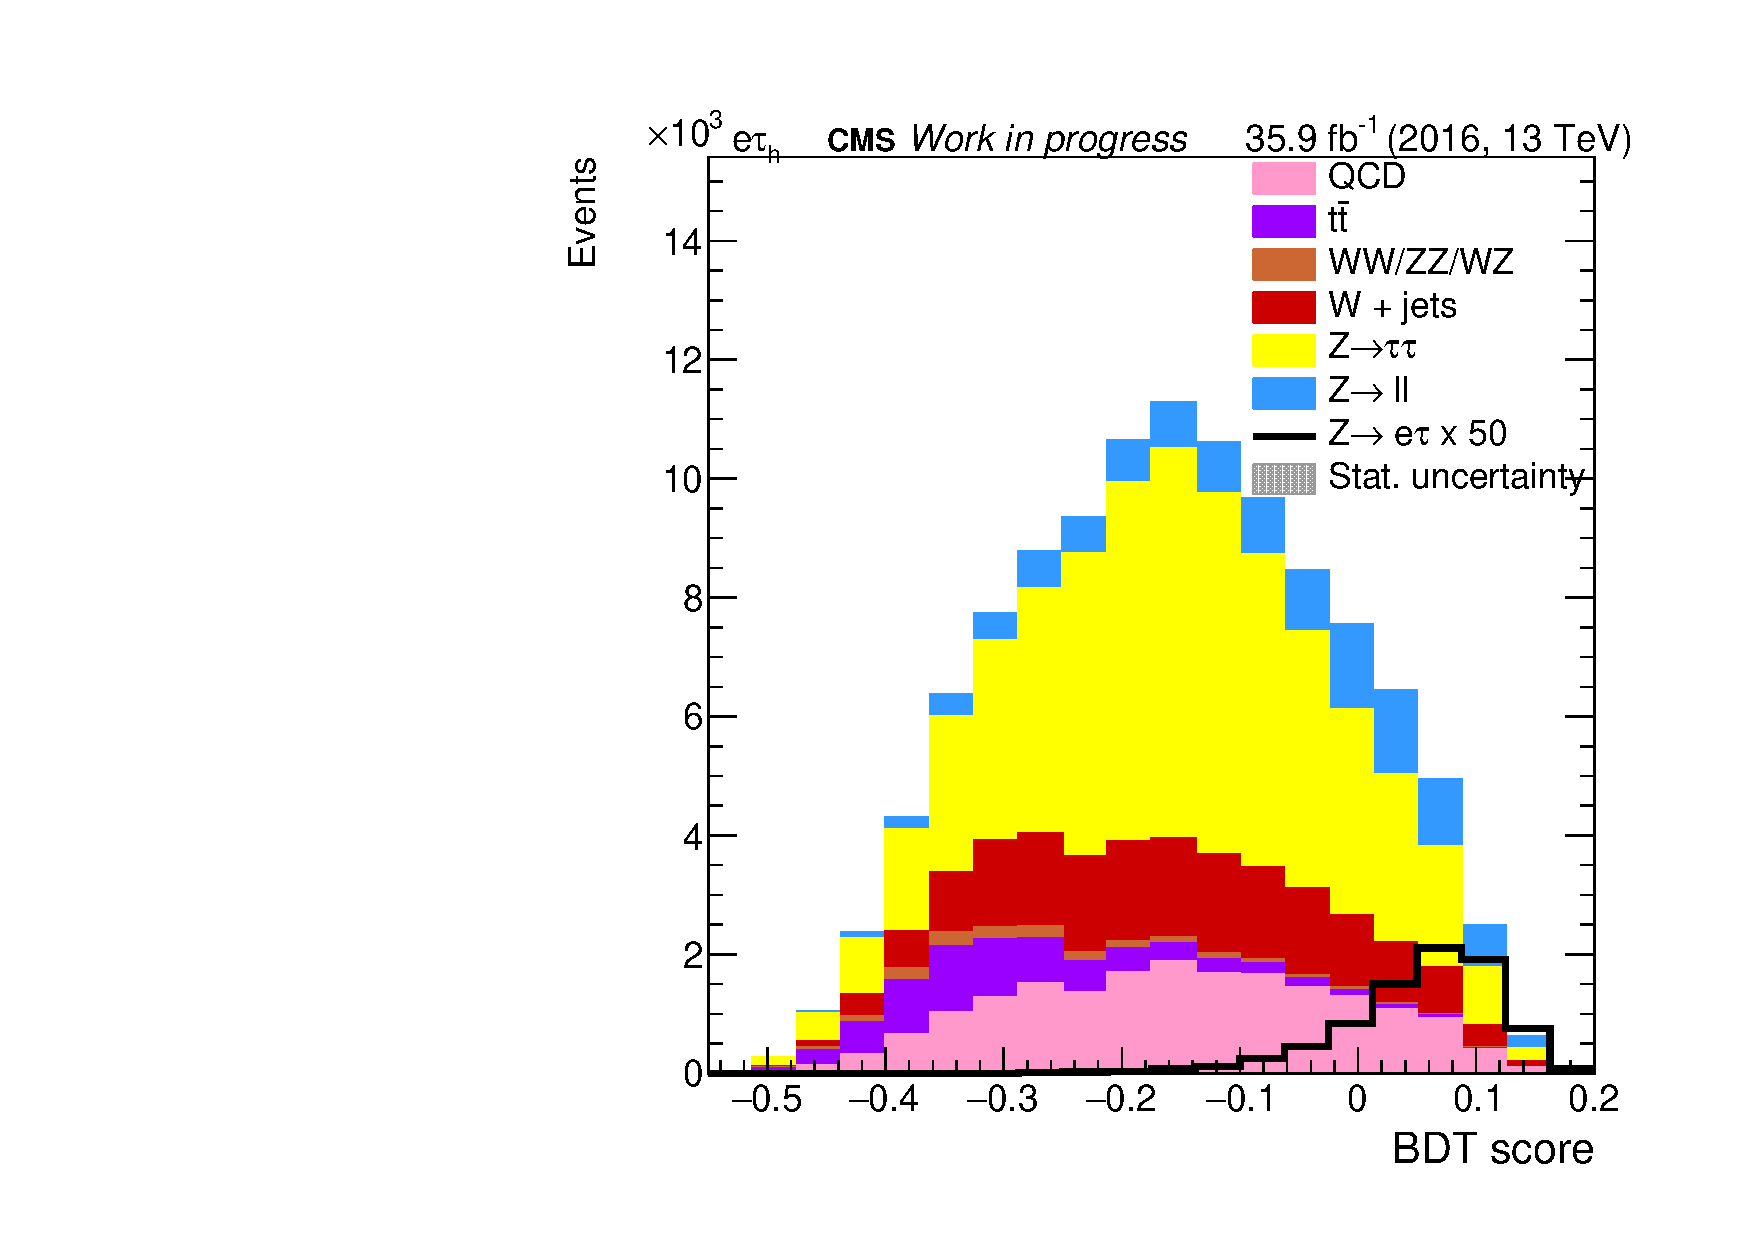
\includegraphics[width=\linewidth]{plots/et/BDTScore.pdf}\par 
		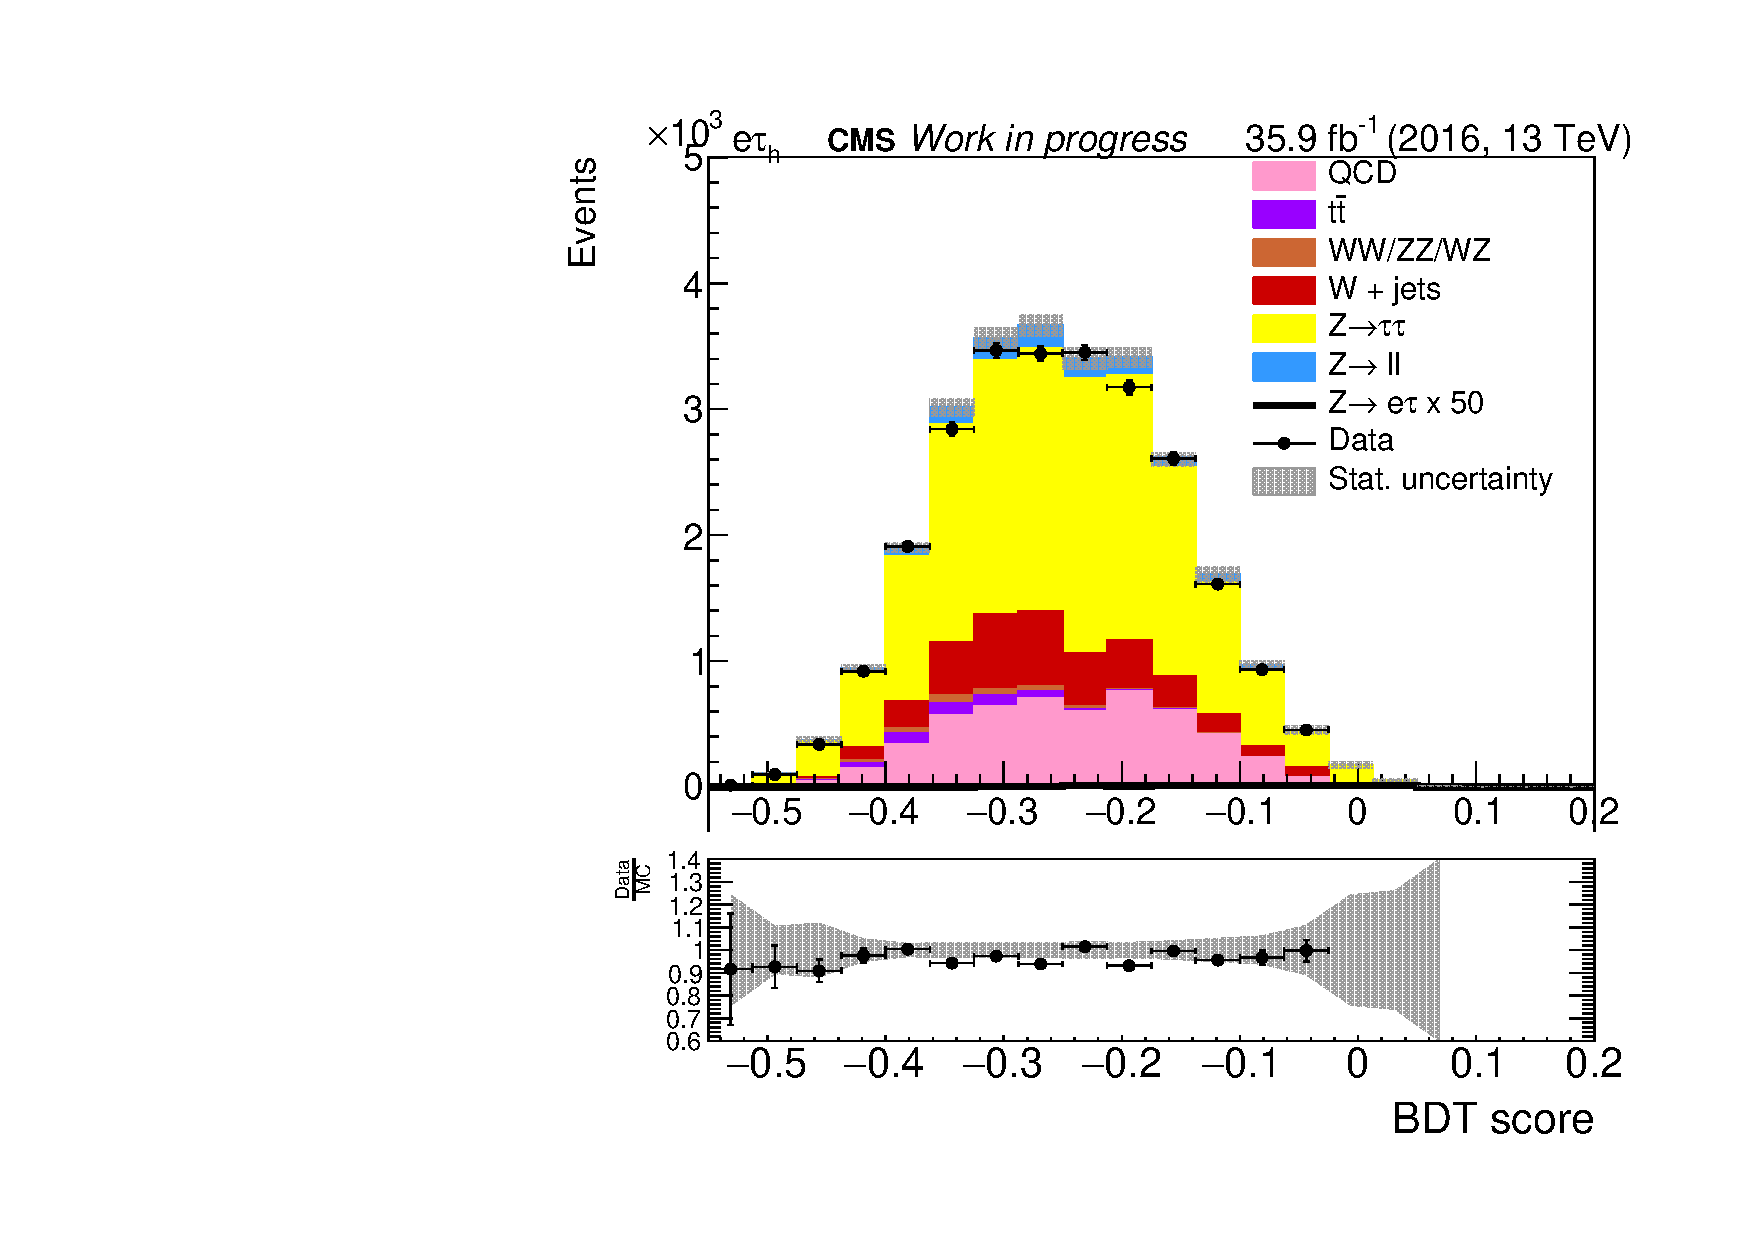
\includegraphics[width=\linewidth]{plots/et/BDTScore_ZTTCR}\par
	\end{multicols}	

	\begin{multicols}{2}
		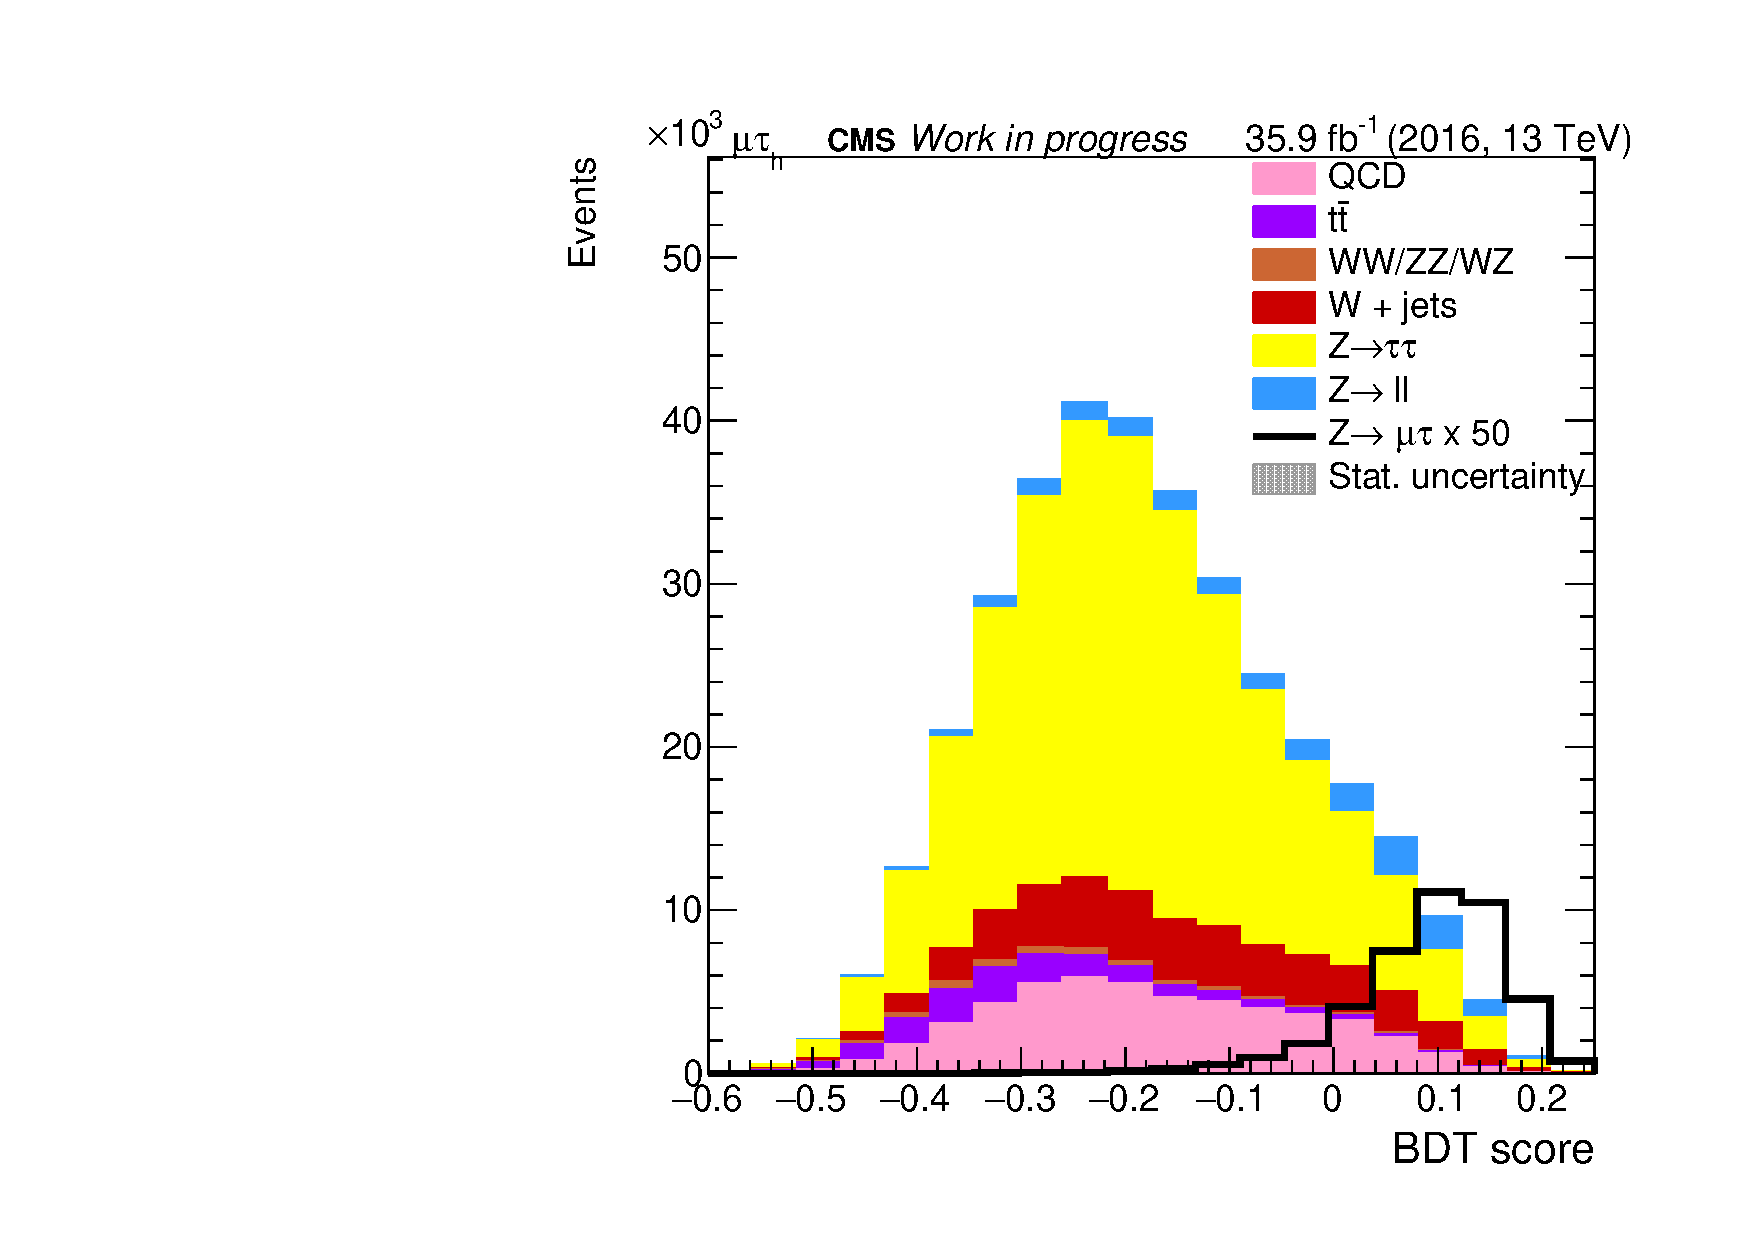
\includegraphics[width=\linewidth]{plots/mt/BDTScore.pdf}\par 
		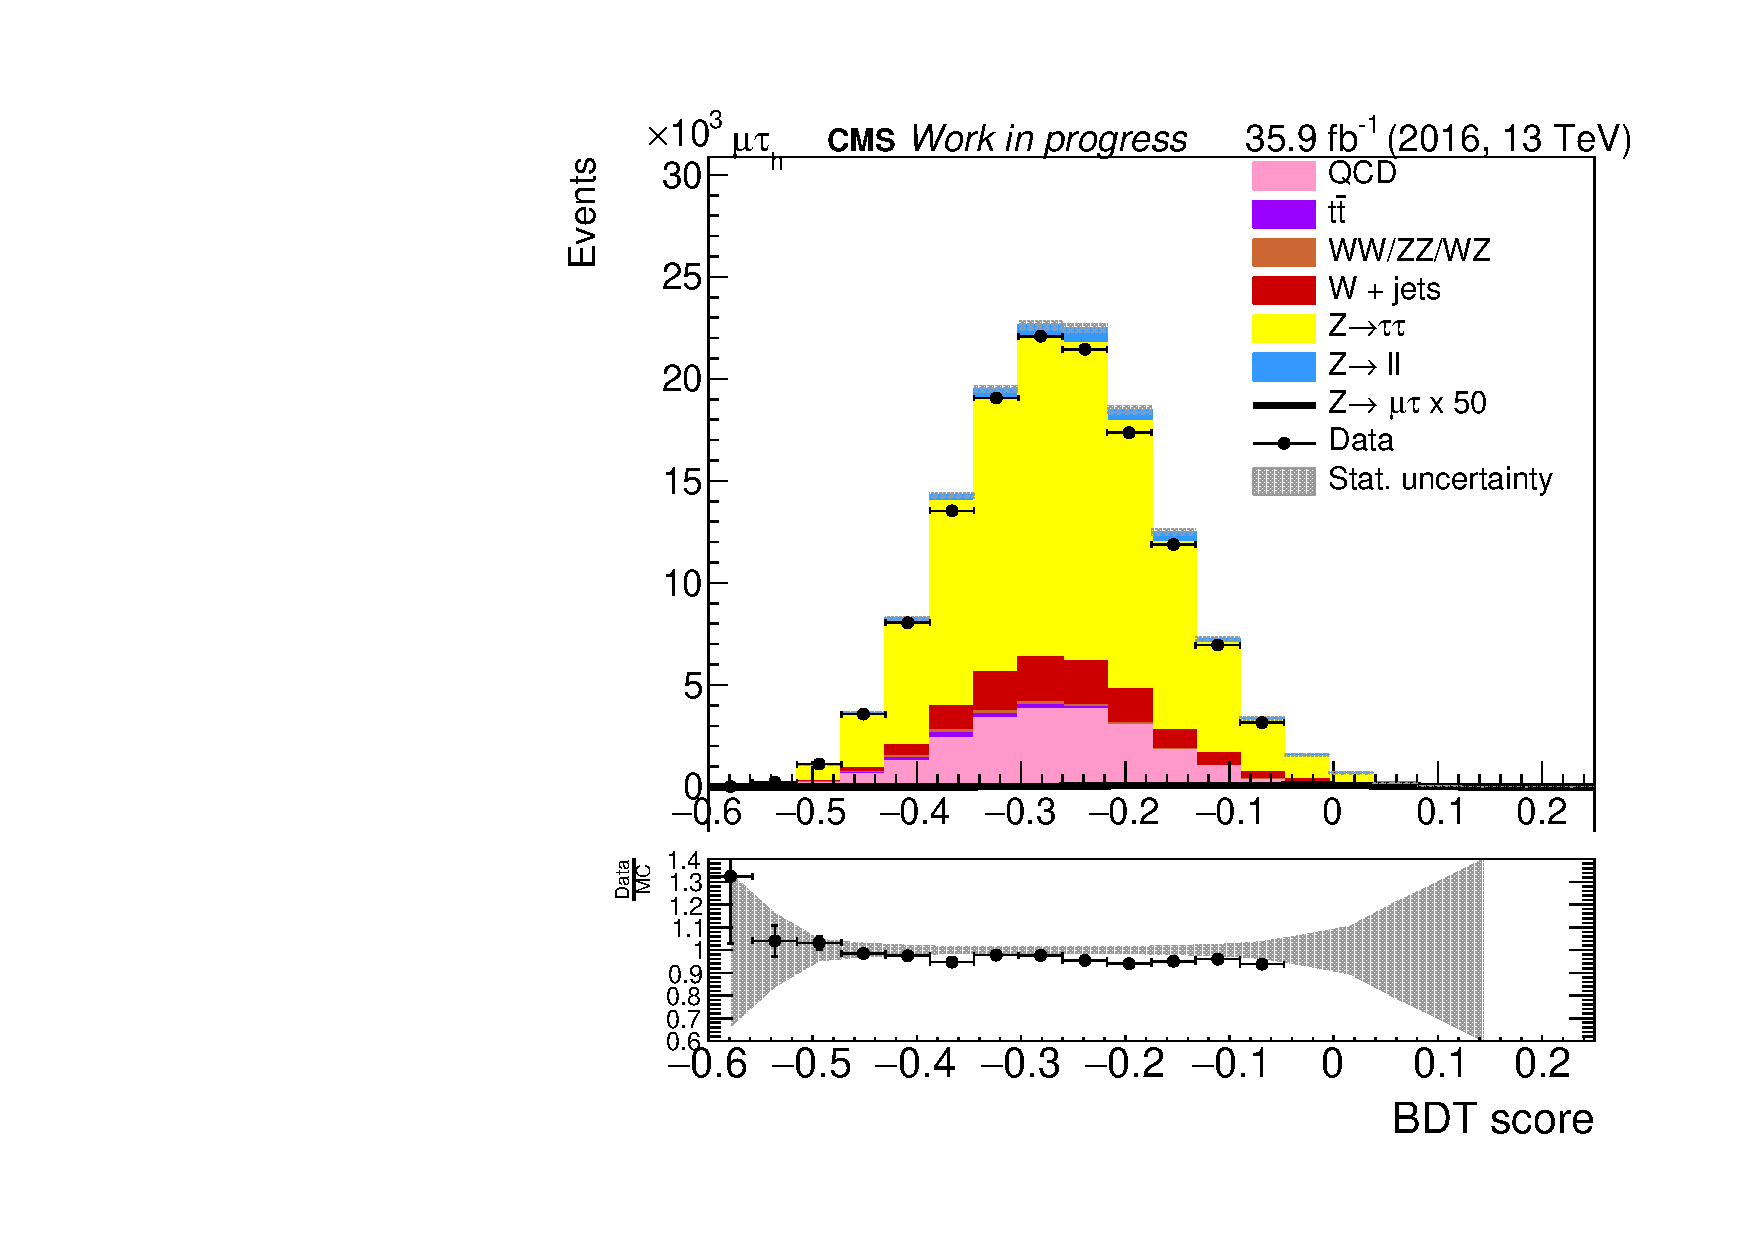
\includegraphics[width=\linewidth]{plots/mt/BDTScore_ZTTCR}\par
	\end{multicols}		

	\caption[BDT score]{\gls{BDT} score for the final state $e\mu$, $e\tau$ and $\mu\tau$, one the left inclusive plots with signal, on the right signal free unblinded plots with events \gls{m_vis} $< 60$ GeV and a ratio plot of \gls{MC} and data with the grey band as statistical uncertainty}
	\label{fig:fig_3_11}
\end{figure}

For the $e\mu$ final state the \gls{BDT} score shows a well separation of background and signal, for the $e\tau$ and $\mu\tau$ final state the discrimination power of the \gls{BDT} score is lower. The difference in separation power is caused by the challenge of the reconstruction of \gls{TAUH}. In the $e\mu$ final state, both leptons are prompt, well isolated and in events of the signal no neutrinos are involved. This is reflected in the kinematic distributions of this final state, which have already quite separation power by itself. In the $e\tau$ and $\mu\tau$ final state the reconstruction of the \gls{TAUH} is more challenging than the reconstruction of the electron or muon, and gives rise to more uncertainties to deal with. This is reflected in the separation power of distributions of the kinematic parameter, and therefore also in the \gls{BDT} score. 










	


































\clearpage{\pagestyle{empty}\cleardoublepage}

\chapter{Systematic uncertainties}
\label{sec:section_4}

Each measurement in any experiment is limited by uncertainties, which arise from sources specific to the experiment. In this analysis two kind of sources for uncertainties are existing. The first source is the limited power of the \gls{MC} simulation to describe nature perfectly. The second source is the limits on the precision given by the detector systems of \gls{CMS}. These uncertainties influences the prediction of the simulation in two ways. The first one are normalization effects, which affect the prediction on the number of events, which are expected for a process. The second effect are resolution effects, where the uncertainty on the quantity of the analysis propagates through the analysis, and influences the shapes of the distributions of the quantities of interest. The analysis uses the systematic uncertainties from the SM $H\to\tau\tau$ analysis \cite{SMHTT}, which are also relevant for this analysis, and are discussed in the following and summarized in table \ref{tab:tab_4_1}.

\section{Uncertainties of the event selection}

The uncertainties of the event selection arise from the scale factors, which are discussed in section \ref{sec:section_3_4_3}. The uncertainties of lepton selection criteria, including trigger and identification, are estimated for electrons and muons using the tag and probe method measured in $Z \to ee$ / $Z\to \mu\mu$ data \cite{ERECO, MUONRECO}. The uncertainty is 2 \% per lepton. For the \gls{TAUH} selection criteria, including trigger and identification, the uncertainties are estimated using the tag and probe method measured in $Z \to \tau\tau$ data \cite{TAURECO}. The uncertainty on the trigger efficiency is 2 \% and on the identification is 5 \%.

\section{Uncertainties of the background estimation}

The uncertainties on the background estimation either come from the uncertainties of the parameters going into equation \ref{eq:eq_3_3} for the prediction of expected number of events, or from the fits of the data driven estimation methods.  

The uncertainty on the measured luminosity of the period of 2016 data taken is estimated to be 2.5\% \cite{LUMI}. For the $Z\to\tau\tau$ background, due to the correction of the yield and background using $Z\to \mu\mu$ data, an uncertainty on the estimation is set to 10\%. The uncertainties from the yields of single top and di-boson production are estimated to be 5\% \cite{singleT} \cite{VV}. In the $e\mu$ final state, in which $W +jets$ is estimated from simulation, the normalization uncertainty arises from misidentification rates of jets to electrons/muons and is set to be 20\%. For the $e\tau$, $\mu\tau$ final state, the uncertainty on the normalization comes from the extrapolation from the same-sign to opposite-sign region and is accounted for 5-10\%. For the \gls{QCD} background, in the $e\mu$ final state the uncertainty on normalization arises from the extrapolation of the same-sign to opposite-sign region and is set to be 10-20\%. For the $e\tau$/$\mu\tau$ final state the uncertainty on the extrapolation is 20\%. 

\section{Uncertainty of the energy scale}

The measurement of the energy is limited by the resolution of the detector subsystem and affects the reconstruction of the physical objects. \\

The uncertainty on the energy scale of the electron depends on the position in the detector (barrel/endcap) and is estimated to be 1-2.5\%. With 0.2\% the muon energy scale uncertainty is negligible small and not considered. Not depending on the decay mode of the hadronic $\tau$, the uncertainty on the energy scale is estimated to be 1.2\%. The uncertainties on the jet energy scale are dependent on \gls{eta} and \gls{pT}. Uncertainties on the $E_T^{miss}$ scale \cite{METRECO} arise from unclustered energy entries in the calorimeters. Also jet energy scale uncertainties, which affect directly the $E_T^{miss}$ scale are taken into account. The value of the uncertainty is dependent on \gls{pT} and \gls{eta}. Uncertainties arising from the energy scale of leptons faking a hadronic $\tau$ are estimated to be 1-2.5\%.

\section{Uncertainty related to $\tau$ leptons}

Uncertainties on the reconstruction of the $\tau$ leptons arise from the misidenfication rates of \gls{TAUH} and the efficiency of the reconstructed decay modes. For $Z\to ee$ and $Z\to \mu\mu$ processes, in which one of the leptons is misidentified as a \gls{TAUH}, a rate uncertainty of 25/12\% is considered. For jets from quarks or gluons, which are misidentified as \gls{TAUH}, a \gls{pT} dependent rate uncertainty of 20 \% per 100 GeV \gls{pT} is used \cite{TAURECO}. Uncertainties on the efficiency on identification and reconstruction of a specific hadronic decay mode of the \gls{TAUH} are set to be 3\%.


\begin{table}[hbtp]
	\centering
	\caption[Systematic uncertainties]{Sources and values of normalization uncertainties in the first part of the table, the shape uncertainties in the second of the table}
	
	\label{tab:tab_4_1}
		\begin{tabular}{l|l|l}
		Uncertainty                                & Value in \%             & relevant for final state   \\ \hline
		$e$ identification                             & 2                   & \begin{tabular}{lll} $e\mu$ & $e\tau$  &  \end{tabular}\\
		$\mu$ identification                     & 2                       &   \begin{tabular}{lll} $e\mu$ & & $\quad \mu\tau$ \end{tabular}        \\
		$\tau$ idenfication                        & 5                       & \begin{tabular}{lll} $ $ & \quad $e\tau$& $\mu\tau$ \end{tabular} \\
		$e$ trigger                                  & 2                       & \begin{tabular}{lll} $e\mu$ & $e\tau$  &  \end{tabular}        \\
		$\mu$ trigger                              & 2                       & \begin{tabular}{lll} $e\mu$ & $e\tau$  &  \end{tabular}           \\
		$\tau$ trigger                             & 5                       & \begin{tabular}{lll} $e\mu$ & &  \end{tabular}        \\
		$W + \text{jets}$  normalization           & 20                      & \begin{tabular}{lll} $e\mu$ & $e\tau$  &  \end{tabular}                    \\
		$W + \text{jets}$ extrapolation            & 10                      & \begin{tabular}{lll} $ $ & \quad $e\tau$& $\mu\tau$ \end{tabular}        \\
		QCD normalization                          & 10-20                   & \begin{tabular}{lll} $e\mu$ & &  \end{tabular}                    \\
		QCD extrapolation                          & $20$                    & \begin{tabular}{lll} $ $ & \quad $e\tau$& $\mu\tau$ \end{tabular}       \\
		Diboson normalitzation                     & 5                       &  \begin{tabular}{lll} $e\mu$ & $e\tau$ & $\mu\tau$ \end{tabular} \\
		$Z\to\tau\tau/\ell\ell$ normalization      & 7                       &\begin{tabular}{lll} $e\mu$ & $e\tau$ & $\mu\tau$ \end{tabular} \\
		$t\bar{t}$ normalization                   & 5                       &\begin{tabular}{lll} $e\mu$ & $e\tau$ & $\mu\tau$ \end{tabular}\\ 
		Luminosity                                 & 2.5                     & \begin{tabular}{lll} $e\mu$ & $e\tau$ & $\mu\tau$ \end{tabular}\\ \hline \hline
		$e$ energy scale                           & 1-2.5                   &\begin{tabular}{lll} $e\mu$ & $e\tau$  &  \end{tabular}           \\
		$\tau$ energy scale                        & 1.2                     & \begin{tabular}{lll} $ $ & \quad $e\tau$& $\mu\tau$ \end{tabular}       \\
		Jet energy scale                           & \gls{pT}, \gls{eta} dependent &\begin{tabular}{lll} $e\mu$ & $e\tau$ & $\mu\tau$ \end{tabular} \\
		$p_{T}^{miss}$ energy scale                & \gls{pT}, \gls{eta} dependent & \begin{tabular}{lll} $e\mu$ & $e\tau$ & $\mu\tau$ \end{tabular} \\
		$e$ misidentified as $\tau$ energy scale     & 3                       &  \begin{tabular}{lll} $ $ & \quad $e\tau$& $\mu\tau$ \end{tabular}      \\
		$\mu$ misidentified as $\tau$ energy scale & 1.3                     & \begin{tabular}{lll} $ $ & \quad $e\tau$& $\mu\tau$ \end{tabular}     \\
		$e$ misidentified as $\tau$ rate              & 20                      &  \begin{tabular}{lll} $ $ & \quad $e\tau$& $\mu\tau$ \end{tabular}        \\
		$\mu$ misidentified as $\tau$ rate          & 25                      & \begin{tabular}{lll} $ $ & \quad $e\tau$& $\mu\tau$ \end{tabular}        \\
		Jet misidentified as $\tau$ rate           & 20                      & \begin{tabular}{lll} $ $ & \quad $e\tau$& $\mu\tau$ \end{tabular}        \\
		$\tau$ decay mode reconstruction           & 3                       & \begin{tabular}{lll} $ $ & \quad $e\tau$& $\mu\tau$ \end{tabular}   \\    
	\end{tabular}
\end{table}

\clearpage{\pagestyle{empty}\cleardoublepage}

\chapter{Statistical analysis and results}
The statistical interpretation of the extracted distribution from events of simulation and data enables the possibility to make a statement about \gls{LFV} in nature. For the interpretation of data and simulation two hypotheses are made: the background only hypothesis (no \gls{LFV} in nature) and the signal + background hypothesis (\gls{LFV} occur in nature). In this analysis the evaluation of the hypotheses  is done with the $CL_s$ method \cite{CLS}, which is recommended by the \gls{CMS} collaboration. 

\section{Maximum likelihood approach and the $CL_s$ method}
\label{sec:section_5_1}

The measured value of a physical quantity is a random variable, which distribution can be described by probability densities. For a counting experiment the number $n$ of counted events for a specific value of the physical quantity is described by the Poisson distribution $p(n) = \frac{\lambda^{n}}{n!}e^{-\lambda}$ with $\lambda$ as the expected value of the counted events. For the case $n$ is measured in the experiment and $\lambda$ is unknown the probability density is called likelihood function $\mathcal{L}$ \cite{LIKELIHOOD}. For this analysis, which is a multi-bin counting experiment, the Poisson distributed likelihood function is defined as

\begin{equation}
	\label{eq:eq_5_1}
	\mathcal{L}(\text{data} | \mu, \vec{\theta}) = \Pi_{i} \frac{(\mu s_i+ b_i)^{n_i}}{n_i!} e^{-\mu s_i +b_i} \cdot p(\vec{\theta_i}).
\end{equation}

The first term is the Poisson distribution, where the expected bin content $i$ is parametrized with $s$ signal events and $b$ background events and a floating signal strength parameter $\mu$. This signal strength is $\mu = 0$ for the background hypothesis and $\mu>0$ for the signal + background hypothesis. Systematic uncertainties are parametrized by the floating parameter vector $\vec{\theta}$ and are described by the prior function $p$.  \\

To evaluate the experiment, the so-called test statistic $\tilde{q}_{\mu}$ is defined like 

\begin{equation}
	\label{eq:eq_5_2}
	\tilde{q}_{\mu} = -2\ln{\frac{\mathcal{L}(\text{data} | \mu, \hat{\vec{\theta_{\mu}}})}{\mathcal{L}(\text{data} | \hat{\mu}, \hat{\vec{\theta}})}}
\end{equation}

with $\mathcal{L}(\text{data} | \hat{\mu}, \hat{\vec{\theta}})$ as the global maximum of the likelihood function and $\mathcal{L}(\text{data} | \mu, \hat{\vec{\theta_{\mu}}})$ as the likelihood function, where the nuisance parameters $\hat{\vec{\theta_{\mu}}}$ are tuned to maximize the likelihood in dependence of $\mu$. For the evaluation of the hypotheses the p-values are calculated for both hypotheses. The p-values quantify the probability to find a $\tilde{q}_{\mu} > \tilde{q}_{\mu}^{obs}$ for a given value of $\mu$, where $\tilde{q}_{\mu}$ is distributed according to a probability density $f(\tilde{q}_{\mu})$, and can be calculated using

\begin{equation}
	\label{eq:eq_5_3}
	p_{\mu} = P(\tilde{q}_{\mu} > \tilde{q}_{\mu}^{obs}) = \int_{\tilde{q}_{\mu}^{obs}}^{\infty} f(\tilde{q}_{\mu}) d\tilde{q}_{\mu}.
\end{equation}

For the background hypotheses with $\mu = 0$ the p-value is defined like $p_b = p_{\mu = 0}$ and for the signal + background hypotheses with $\mu>0$ the p-value is defined like $p_s = p_{\mu>0}$. From the ratio of the p-values, the $CL_s$ classifier is defined like

\begin{equation}
	\label{eq:eq_5_4}
	CL_s = \frac{p_s}{p_b}
\end{equation}

and can used for the evaluation of the hypotheses. For a given $\mu$, demanding for example $CL_{s} < \alpha$, the signal hypotheses can be excluded with a $1-\alpha$ confidence level. To make a statement about the values of $\mu$, it is common to demand $CL_{s} < 0.05$ and tune $\mu$ until this value is reached. This value of $\mu_{CL_s = 0.05}$ and all values above can then be excluded with a confidence level of 95\%.

\section{Interpretation of the analysis}
\label{sec:section_5_2}

In this analysis the \gls{BDT} score, which is discussed in section \ref{sec:section_3_5}, is used as the discriminating variable for the counting experiment. The \gls{BDT} score is analyzed in bins of three categories, which are described in section \ref{sec:section_3_2_3}. As nuisance parameter $\vec{\theta}$ the systematic uncertainties discussed in section \ref{sec:section_4} are used.\\

The analysis is interpreted in terms of the expected limit on the signal strength $\mu_{exp}$. The calculation of $\mu_{exp}$ follows the description of section \ref{sec:section_5_1} for $\mu_{CL_s = 0.05}$, but instead of evaluating data events, an Asimov data set \cite{ASIMOV} is used. The Asimov data set is a toy data set generated with the model expectation for a given $\mu$ and the nuisance parameter $\vec{\theta}$. In this case the Asimov data set is generated for the background-only hypothesis with $\mu = 0$. The expected limit quantifies the power of the analysis of setting the constraint on the signal strength, if the background only hypotheses is realized. \\

The constraint on the signal strength can be translated into a constraint on the $\text{BR}(Z\to\text{LFV})$ with $\text{LFV} \in (e\mu, e\tau, \mu\tau)$. In the signal expectation $s$, according to equation \ref{eq:eq_3_3}, the limit on the branching ratios of previous analysis is used. Setting a constraint on the signal strength $\mu$ also set a constraint on the signal expectation $s$. So the expected limit on the branching ratio $\text{BR}_{exp}(Z\to\text{LFV})$ is related to the expected limit on the signal strength $\mu_{exp}$ via 

\begin{equation}
	\text{BR}(Z\to\text{LFV}) \cdot \mu_{exp} > \text{BR}_{exp}(Z\to\text{LFV})
\end{equation}

This relation can now be evaluated to judge the sensitivity of the analysis compared to the previous analysis, which set constraints on the branching ratio. For $\mu_{exp} > 1$ the expected branching ratio is not as good as the constraints from the previous analysis, the sensitivity of the previous analysis is not reached yet. For $\mu_{exp} < 1$ the expected limit gives a better constraint on the branching ration compared to the previous analysis, a gain in sensitivity is achieved. 


\section{Results}
\label{sec:section_5_3}

The results of this analysis are given in terms of expected limits on the branching ratio $\text{BR}(Z\to\text{LFV})$ for each final state. \\

The figure \ref{fig:fig_5_1} shows the excepted limits in each category and the combination of all categories. Generally the sensitivity increases for lower jet multiplicity. This is expected, because as shown in the distribution in figure \ref{fig:fig_3_7}, the signal to background ratio gets worse for higher jet multiplicity. In the $e\mu$ final state the change in sensitivity for each category in comparison to the $e\tau$ and $\mu\tau$ final state can be explained with the dominant $t\bar{t}$ background in the multi-jet category for $e\mu$. \\

Also the latest observed limit is shown in comparison to the combined expected limit of this analysis. In the $e\mu$ final state the expected limits give a three times better constraint on the branching ratio than the latest observed limit. And because the latest observed limits lie far above the uncertainty bands of the expected limit of this analysis, a possible excess due to a \gls{LFV} signal could be measured. This gain in sensitivity is expected, because the latest observed limit was measured during the \gls{CMS} Run I with a lower integrated luminosity of $\mathcal{L}_{int} = 19.8$ fb$^{-1}$ compared to the integrated $\mathcal{L}_{int} = 36.9$ fb$^{-1}$ of this analysis. For the $e\tau$ and $\mu\tau$ final state the expected limits on the branching are almost as good, respectively as good as the constraint given by previous analysis. That the limits are not better like in the $e\mu$ final state, can be explained by the fact, that the latest observed limits in this final state were measured with data of the electron-positron collider \gls{LEP}. In an electron-positron collider the initial state of all processes is known, in the case of proton-proton collisions \gls{PDF} have to be used as described in section \ref{sec:section_2_1_2}. With leptons as colliding objects, the \gls{QCD} multi-jet background was not an issue at \gls{LEP}, which gives a much clearer background compared to proton-proton collider. The analysis of the \gls{TAUH} is therefore much more challenging at \gls{LHC}. 

\begin{figure}[htp]
	\centering
	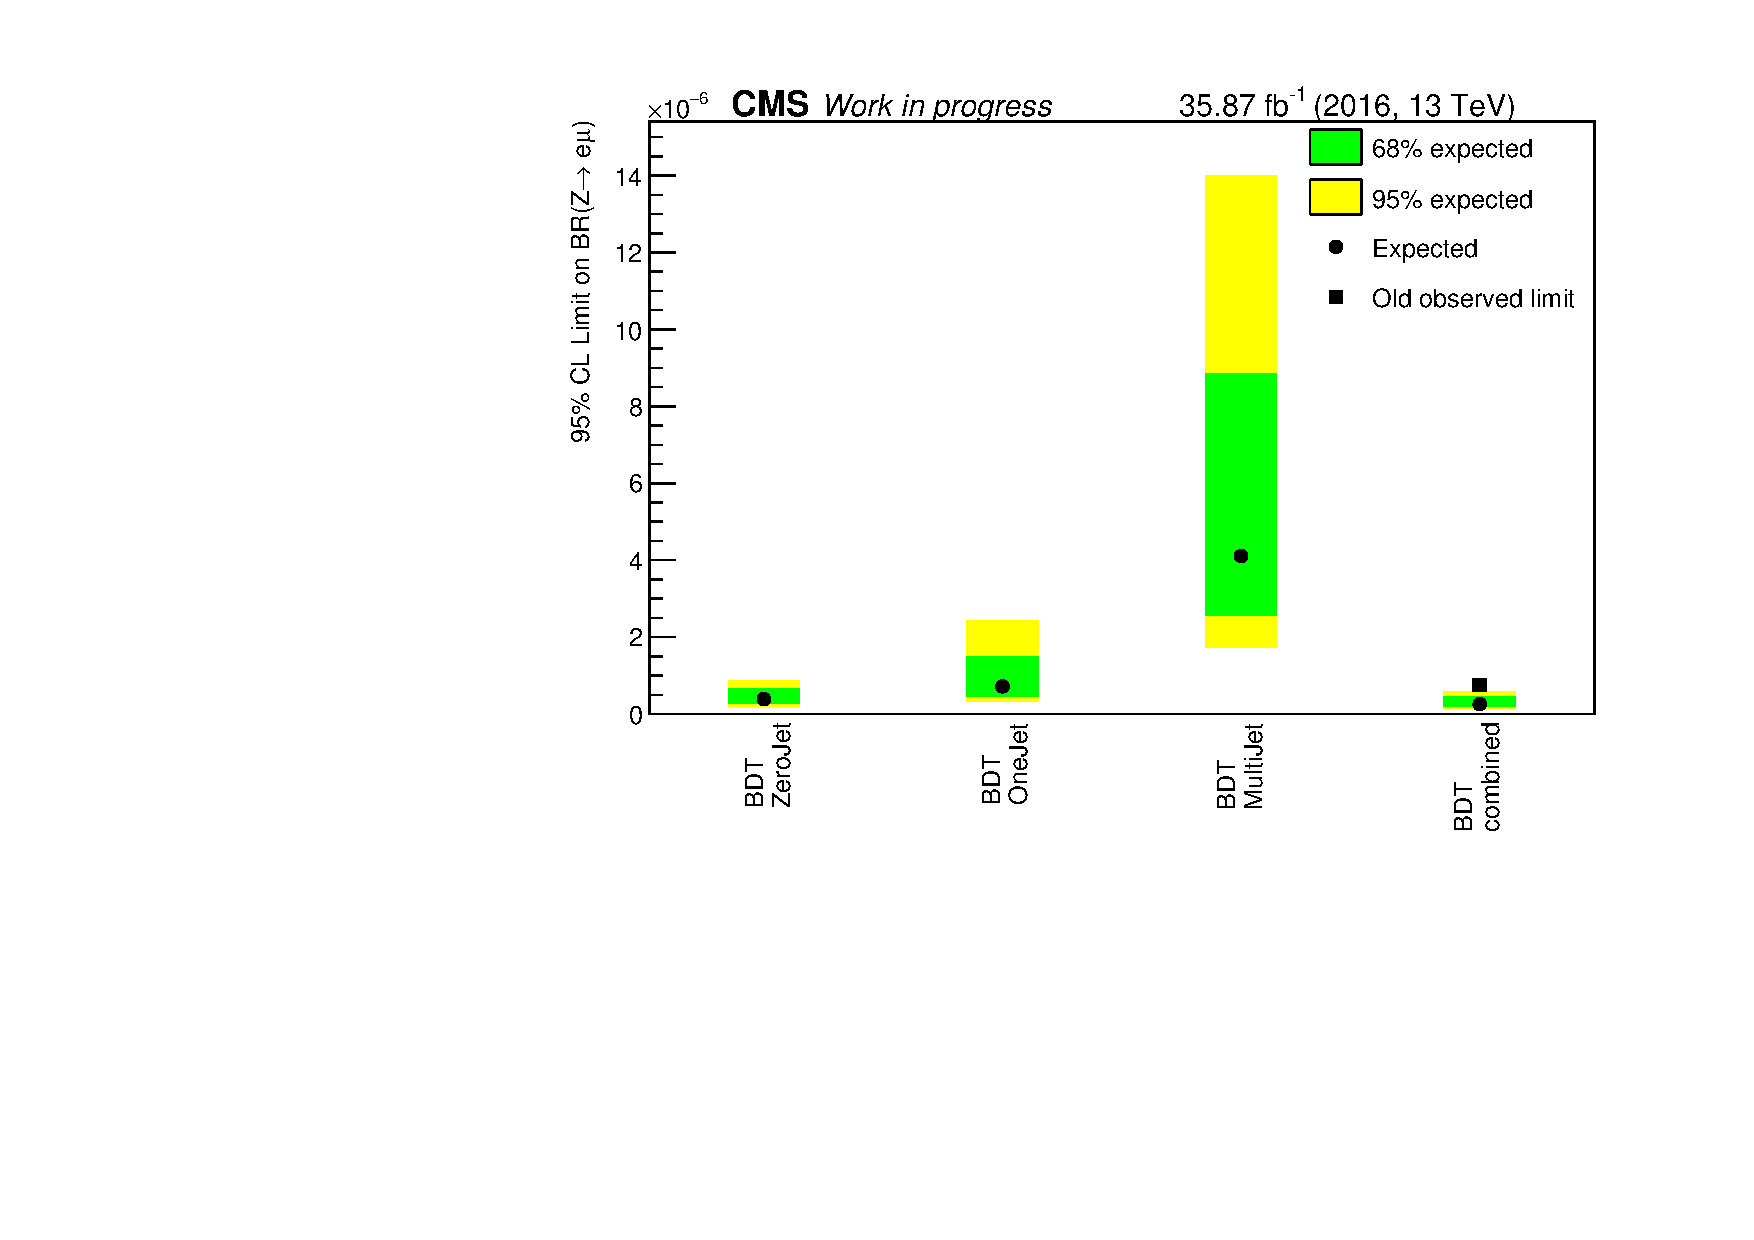
\includegraphics[width=0.6\textwidth]{plots/em/limits.pdf}
	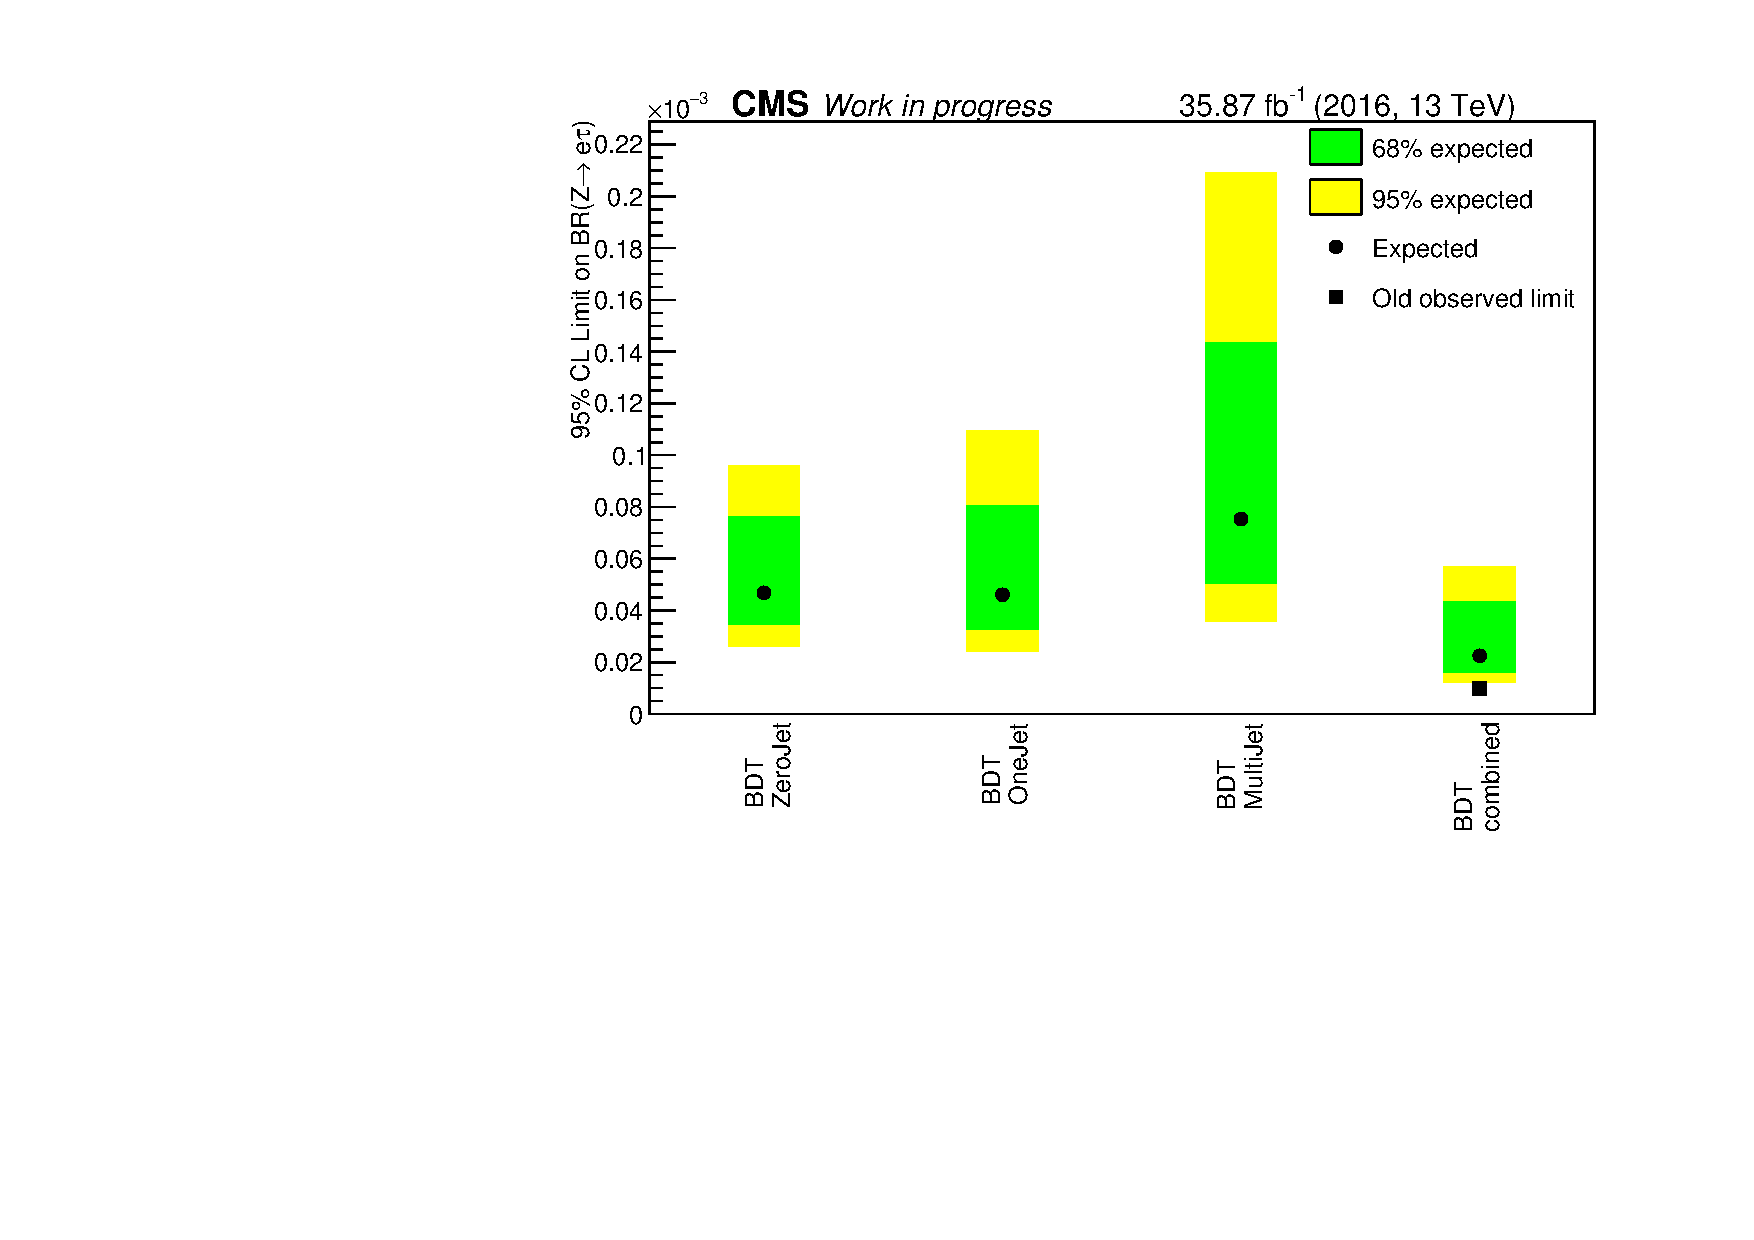
\includegraphics[width=0.6\textwidth]{plots/et/limits.pdf}
	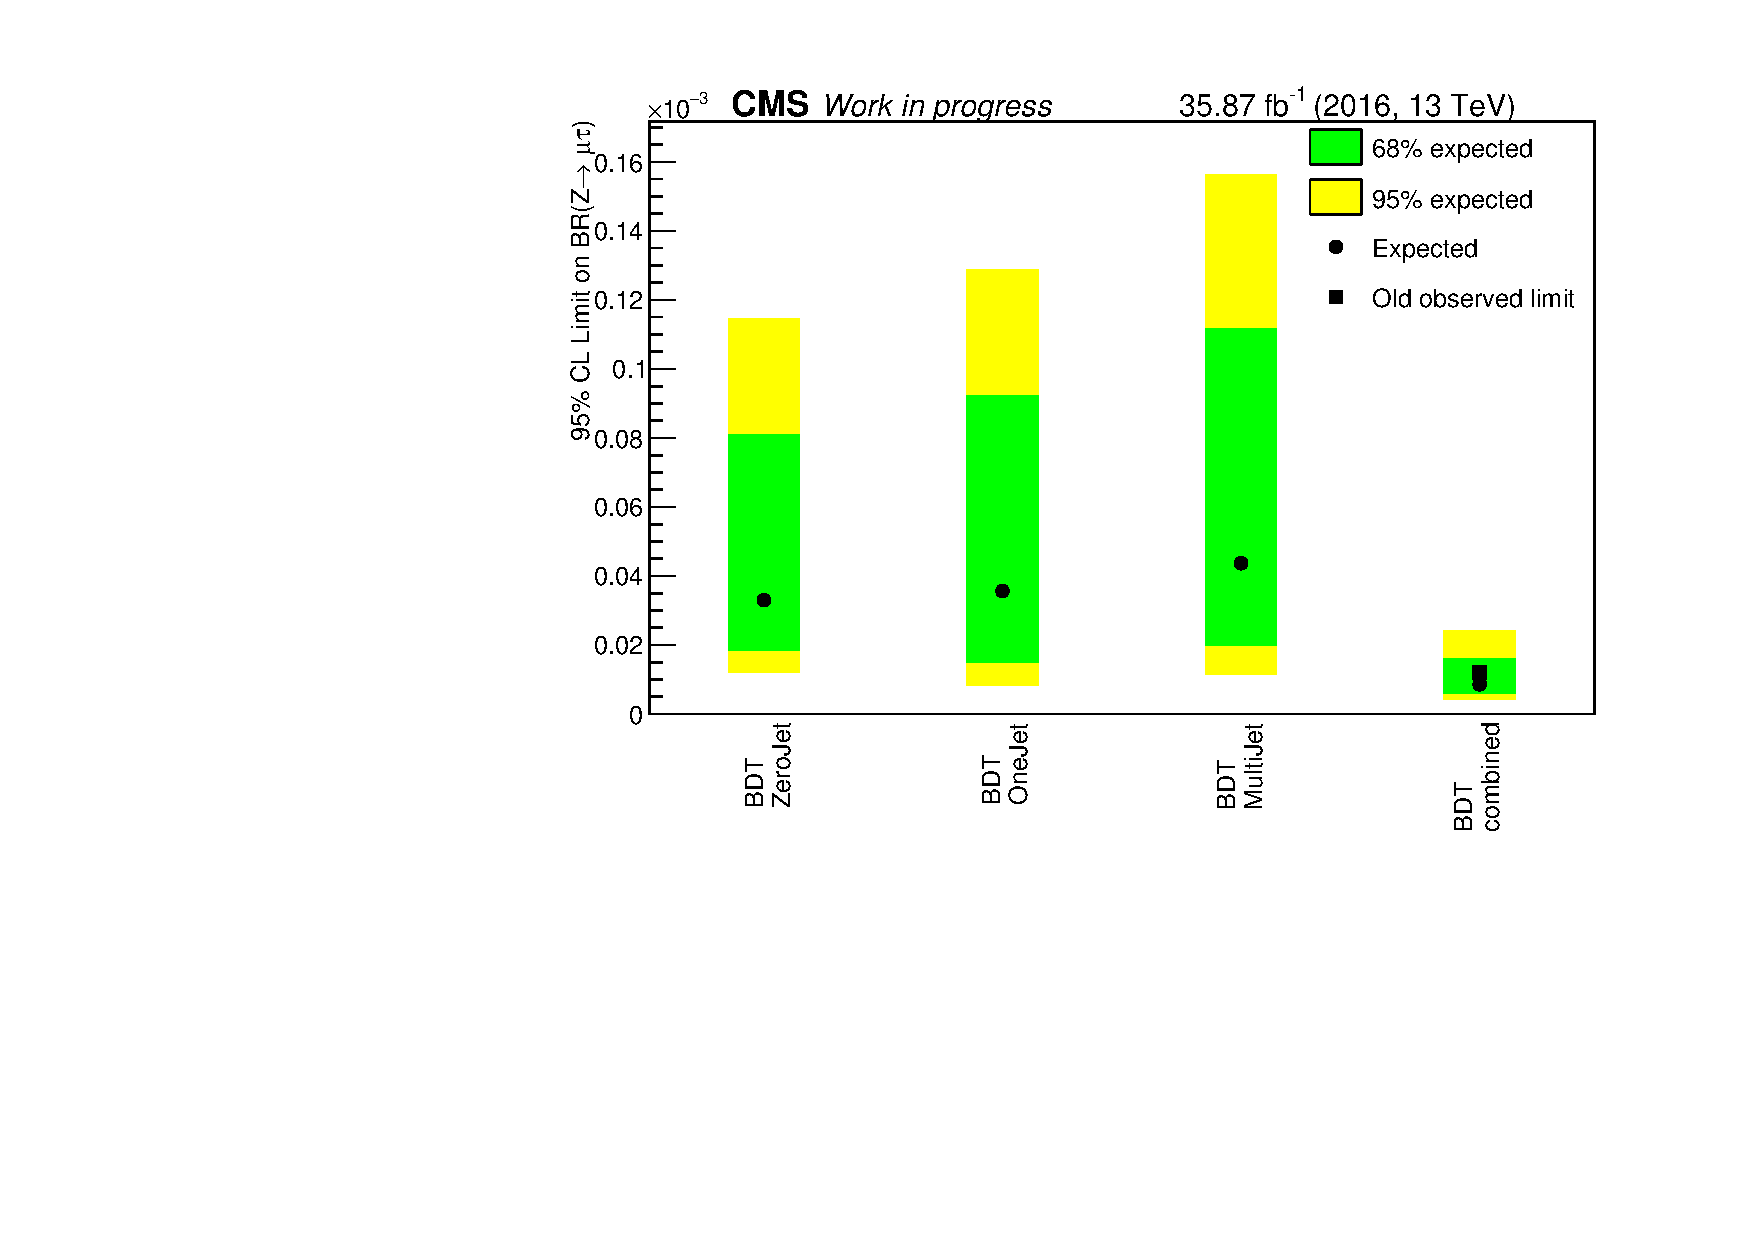
\includegraphics[width=0.6\textwidth]{plots/mt/limits.pdf}

	\caption[Expected limits on the branching ratios]{Expected limits on the branching ratio $\text{BR}(Z\to\text{LFV})$ for each final state. The limits are given for all three categories and the combination of all of them, together with the one/two sigma uncertainty.}
	\label{fig:fig_5_1}
\end{figure}

















\clearpage{\pagestyle{empty}\cleardoublepage}

\chapter{Conclusion and outlook}
The search for \gls{LFV} in decays of Z bosons is performed for the \gls{LHC} run of 2016 with a center of mass energy of $\sqrt{s} = 13$ TeV and with $35.9$ fb$^{-1}$ data recorded by \gls{CMS}. This analysis evaluated the three possible final states of the direct decay of a Z boson, which violates lepton flavour, namely a pair of electron/muon, electron/$\tau$ lepton and muon/$\tau$ lepton. For the $\tau$ lepton the hadronic decaying $\tau$ have been studied because of the high branching ratio $\text{BR}(\tau \to \nu_{\tau} + \text{hadrons}) = 0.63$. \\

Based on an event selection depending on the final state, well isolated and reconstructed leptons are chosen for the analysis. The kinematic parameters of the leptons are used as an input for a training of a sophisticated \gls{MVA} classifier, in the case of this analysis the \gls{BDT} is the choice. Including the systematic uncertainties, which are adopted from the \gls{SM} $H \to \tau\tau$ analysis, upper expected limits on the branching ratios $\text{BR}(Z \to \text{LFV})$ are set in each final state, using the $\text{CL}_{s}$ method. The expected limit in the $e\mu$ final state showed a clear gain in sensitivity in comparison to previous analysis from \gls{CMS}, in the $e\tau$ and $\mu\tau$ final state the expected sensitivity is competitive with previous analysis from \gls{LEP}. \\

At this moment only the hadronic decay mode of the $\tau$ lepton has been studied in this analysis. The inclusion of the leptonic decay mode of the $\tau$ lepton would result in a gain of sensitivity, although at the moment only different flavour final states of the $\tau$ lepton, namely $e\tau \to e\mu$ and $\mu\tau \to \mu e$ could improve the overall result. Same flavour decay like $e\tau \to ee$ and $\mu\tau \to \mu\mu$ are completely dominated by the \gls{DY} $Z\to ee/\mu\mu$ background. \\

In the $e\tau$ and $\mu\tau$ final state the discrimination power is weaker than in the $e\mu$ final state. A better result of separation performance could be achieved by a deep neural network \cite{DNN}. Since the last 5 years the development of deep neural networks, it evolved into the state-of-the-art method in many disciplines, for example picture recognition \cite{DNN2}. Also in high energy physics deep neural networks show an outstanding performance compared to conventional methods, for example in the analysis of Higgs in association of top quarks \cite{DNN3}. \\

The analysis uses the data set recorded by \gls{CMS} of the year 2016. In fact the \gls{LHC} is running in the Run-II period, which also delivered data in 2017 with a luminosity of 45.9 fb$^{-1}$ and is running in 2018 with a luminosity of 53 fb$^{-1}$ \cite{CMSLUMI1718}. So a total Run-II analysis could use approximately 120 fb$^{-1}$ of recorded events, which would be a increase of statistics by factor of 4 in comparison to this analysis and could improve the overall sensitivity. \\

The final step would be a unblinding of the analysis, to really state, if possible deviation from the \gls{SM} can be seen in data, and to set new constraints on the branching ratio, if no deviations are found. 



 



  





\clearpage{\pagestyle{empty}\cleardoublepage}

\begin{appendices}
	\chapter{Input Parameter of the BDT}
	\pagestyle{appendix}
	\label{sec:appendix_A}

The following figures shows the distribution of the kinematic input parameter of the \gls{BDT} training. For each parameter always two plots are shown, first the a signal free plot with events \gls{m_vis} $< 60$ GeV and the inclusive plot with signal drawn. 

\section*{Plot for the $e\mu$ final state}

\begin{figure}[htp]
	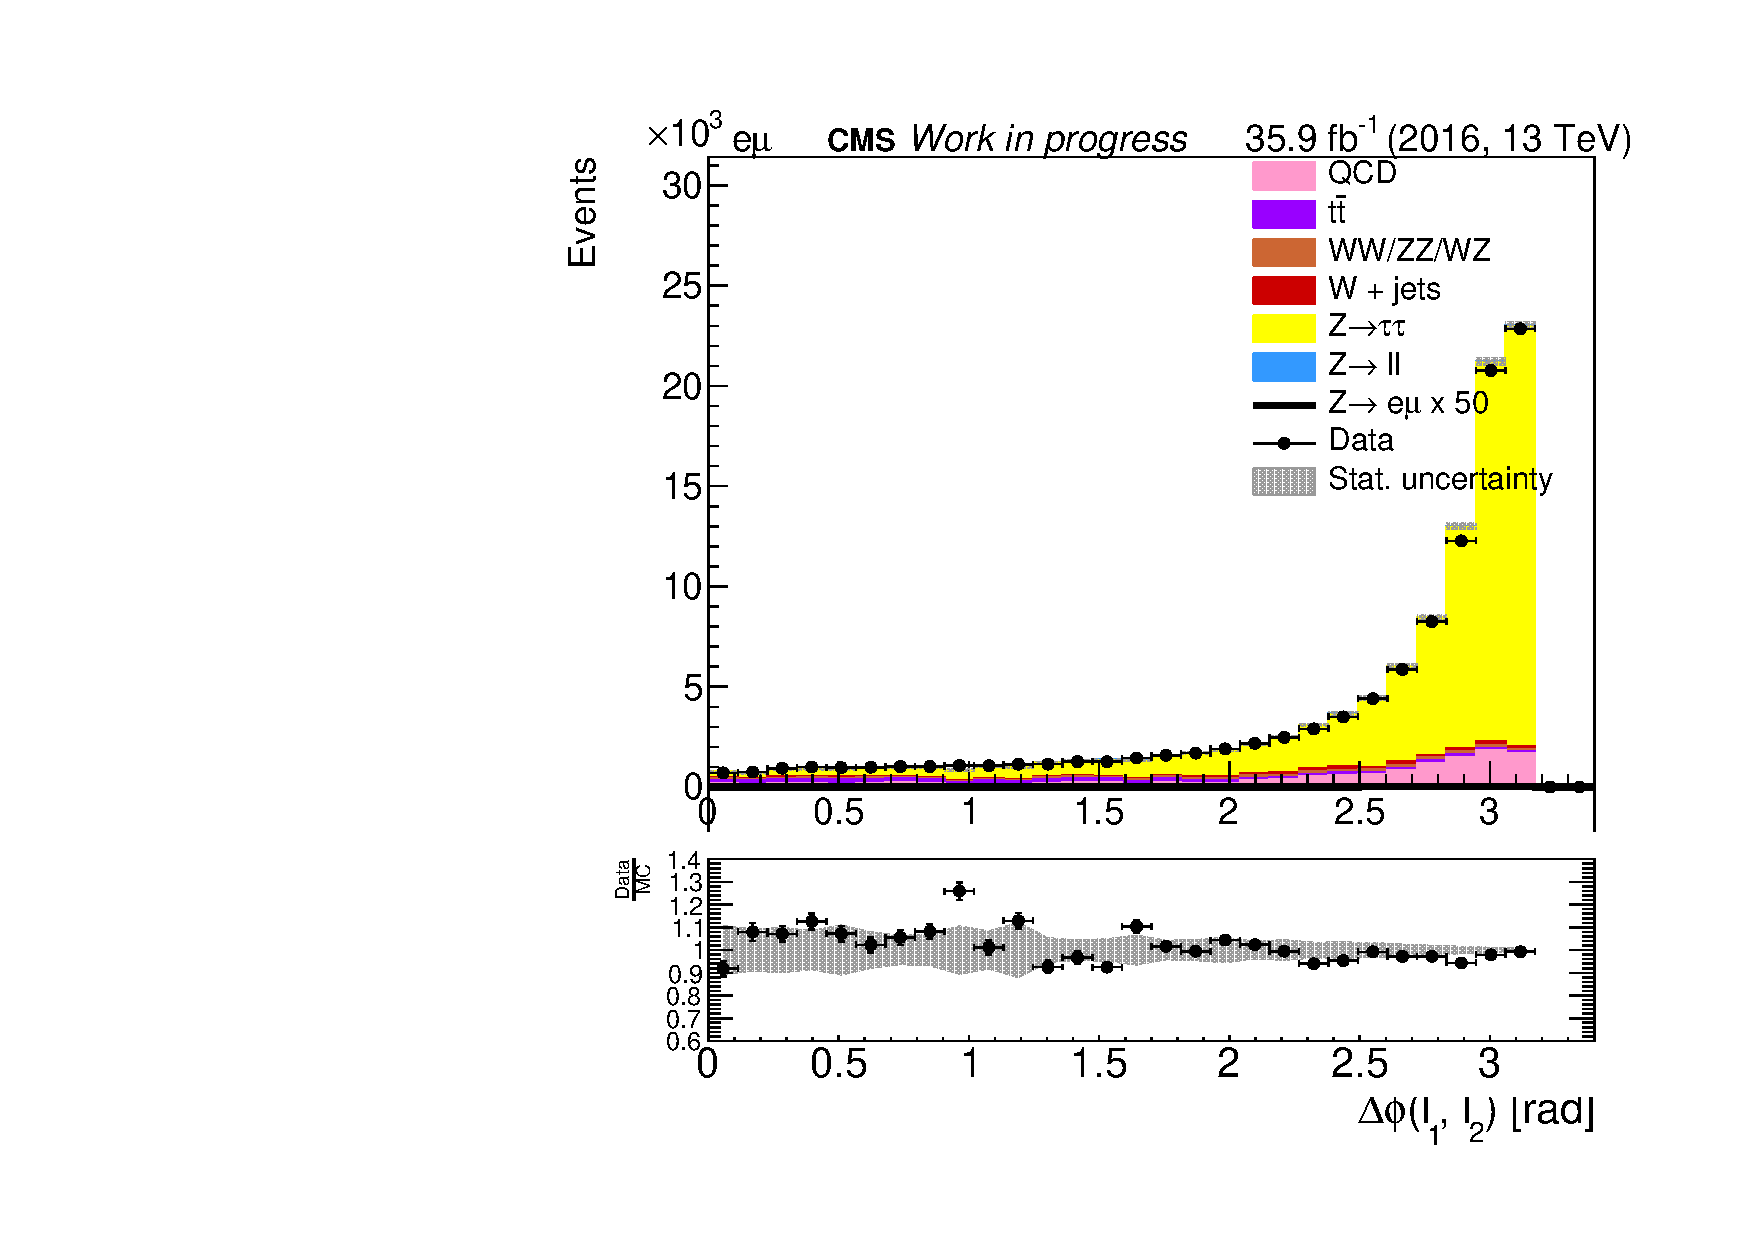
\includegraphics[width=0.45\textwidth]{plots/em/DeltaPhiL1L2_CR.pdf}
	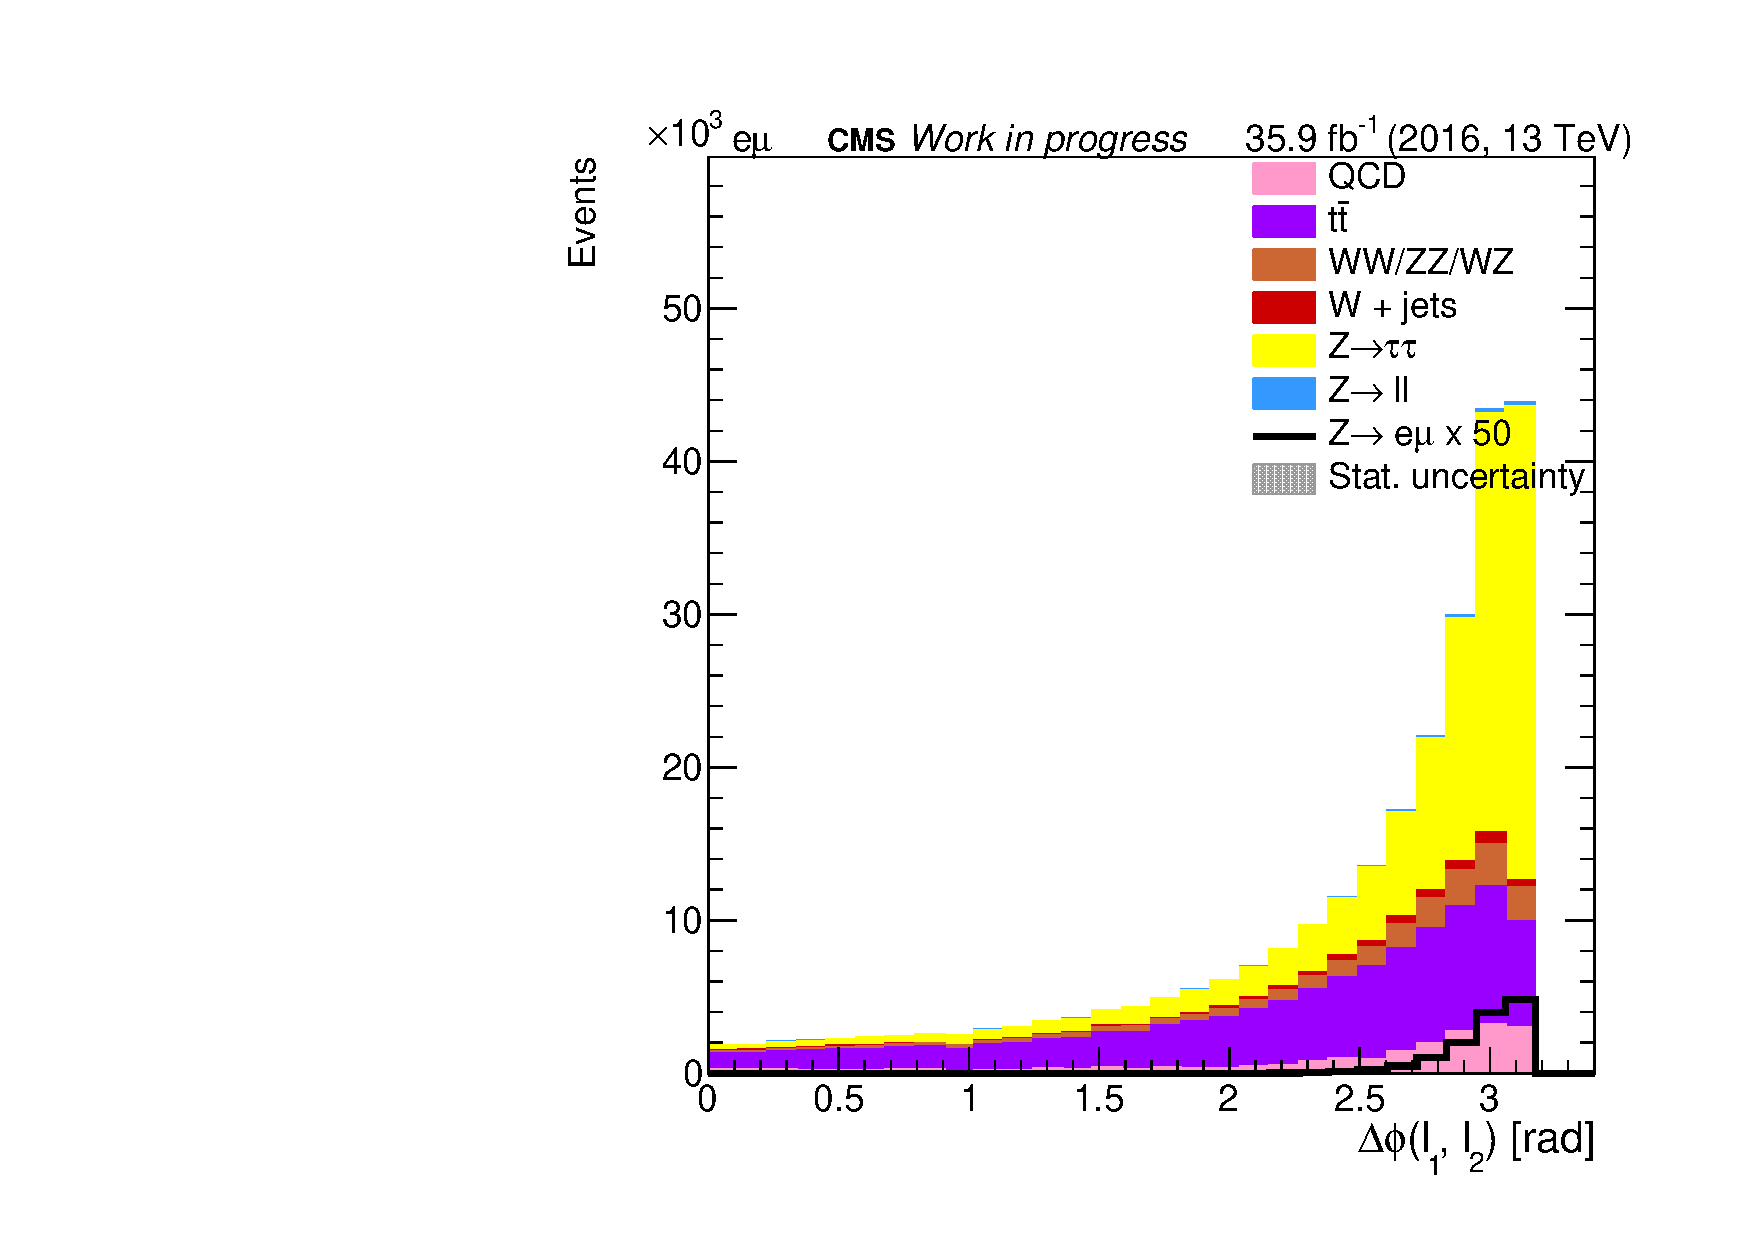
\includegraphics[width=0.45\textwidth]{plots/em/DeltaPhiL1L2_withsignal.pdf}

	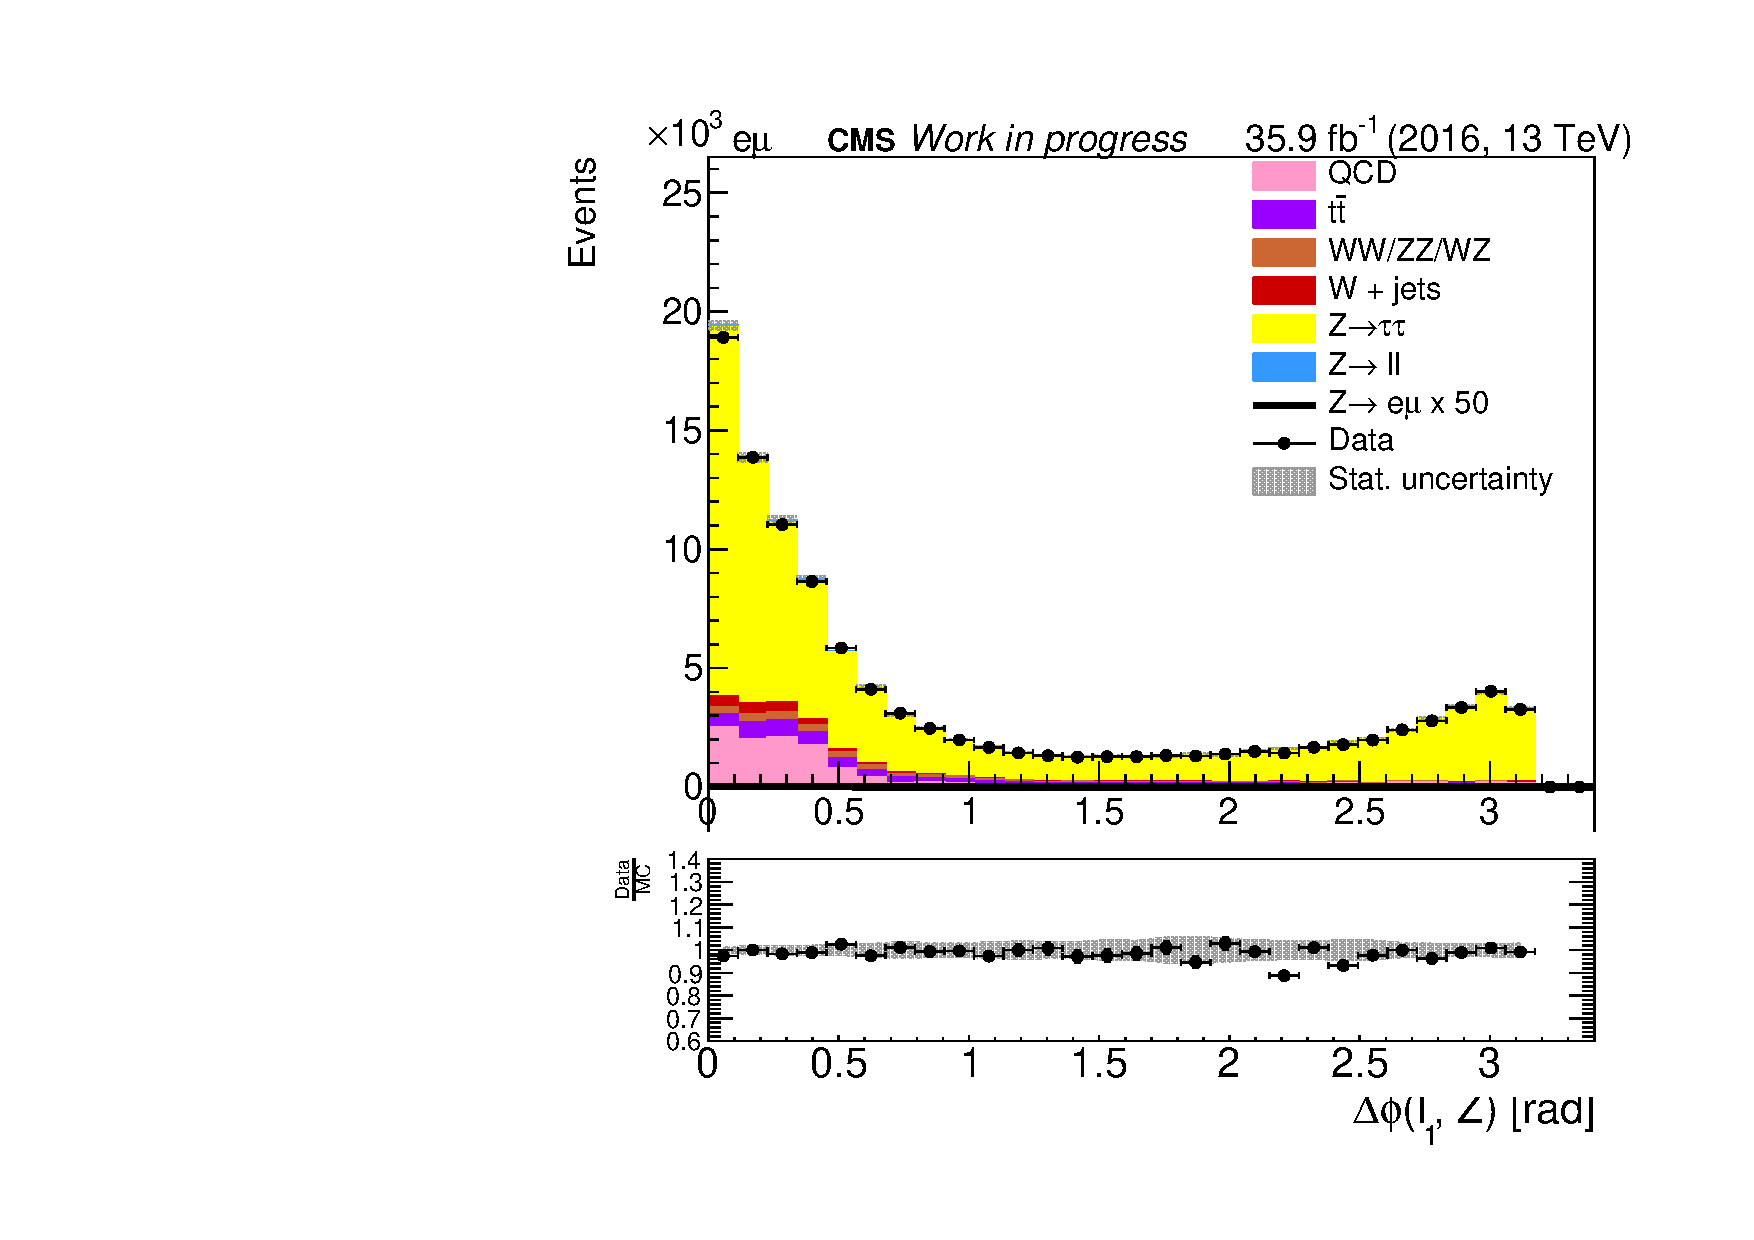
\includegraphics[width=0.45\textwidth]{plots/em/DeltaPhiL1Z_CR.pdf}
	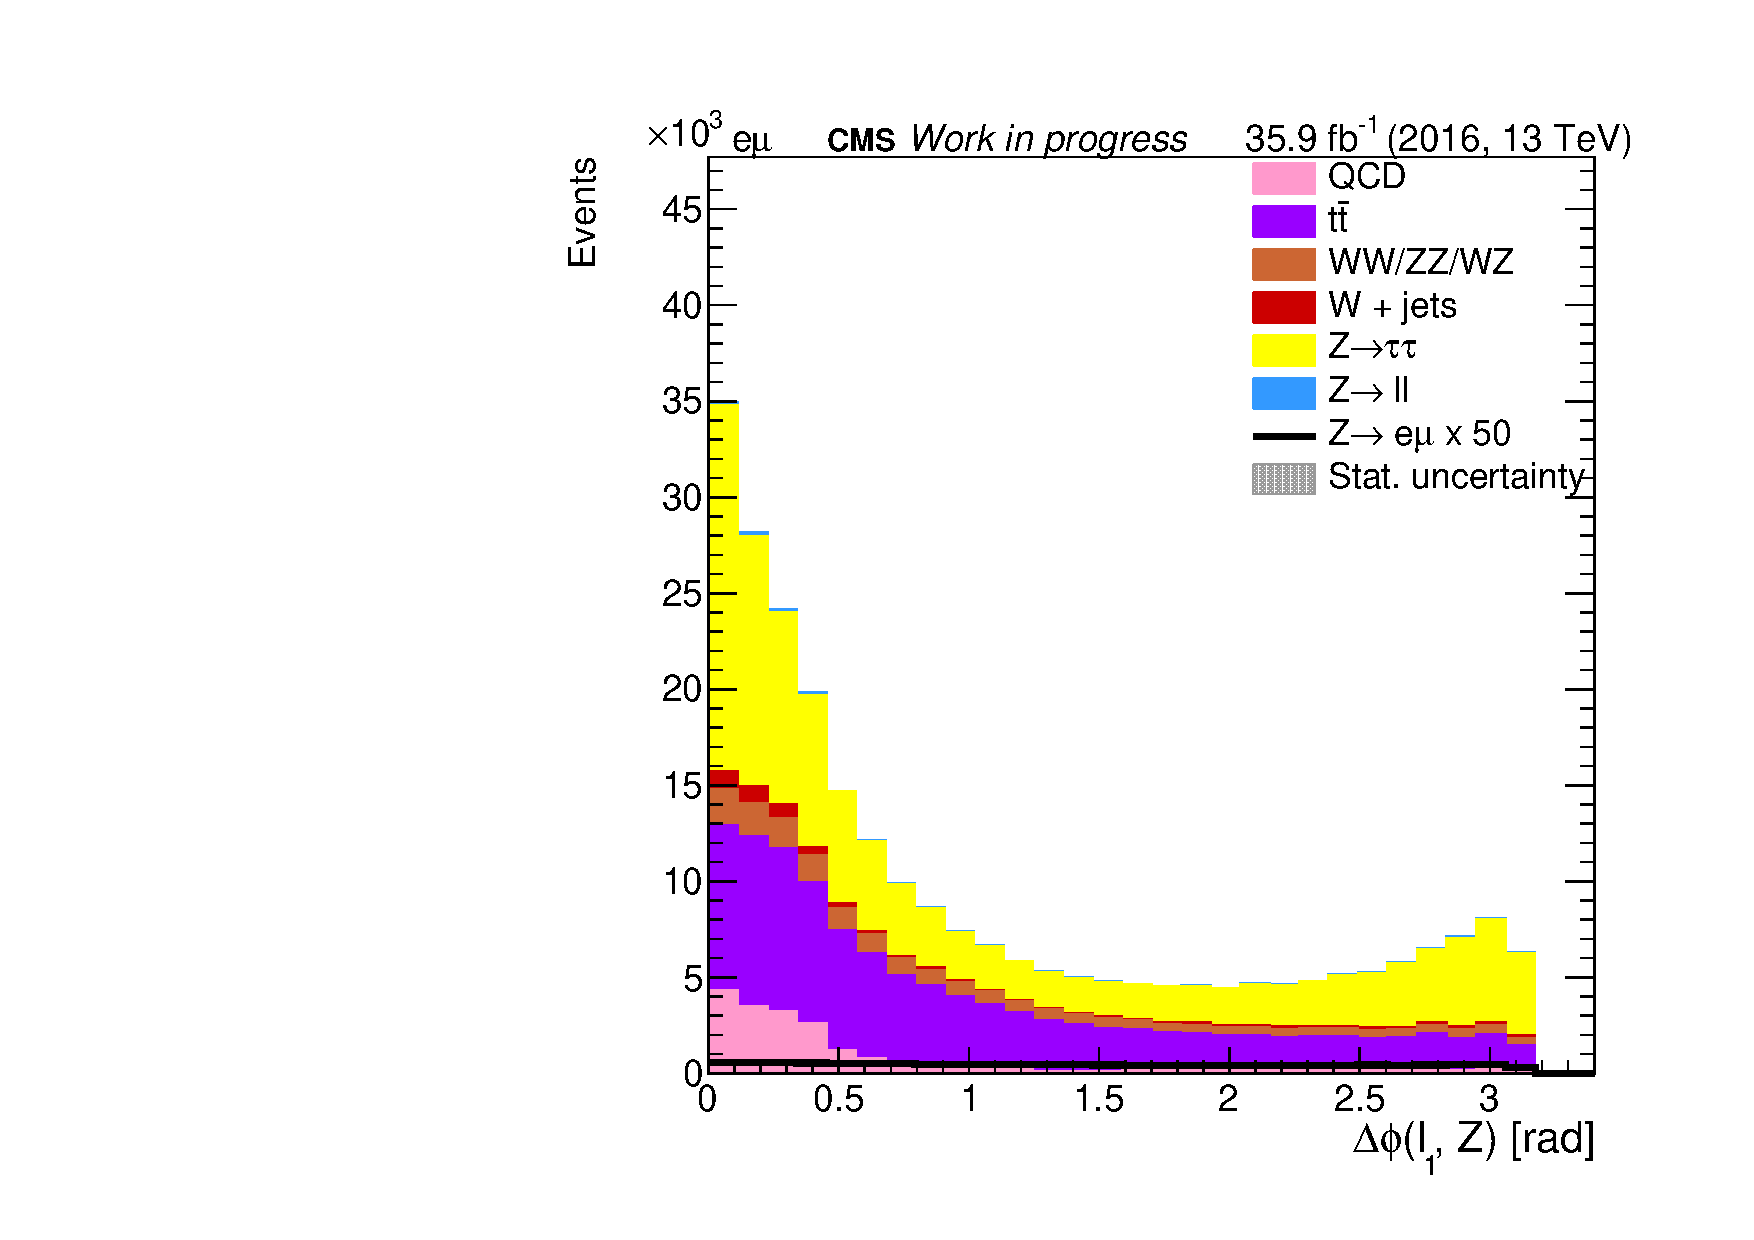
\includegraphics[width=0.45\textwidth]{plots/em/DeltaPhiL1Z_withsignal.pdf}

\end{figure}


\begin{figure}[htp]
	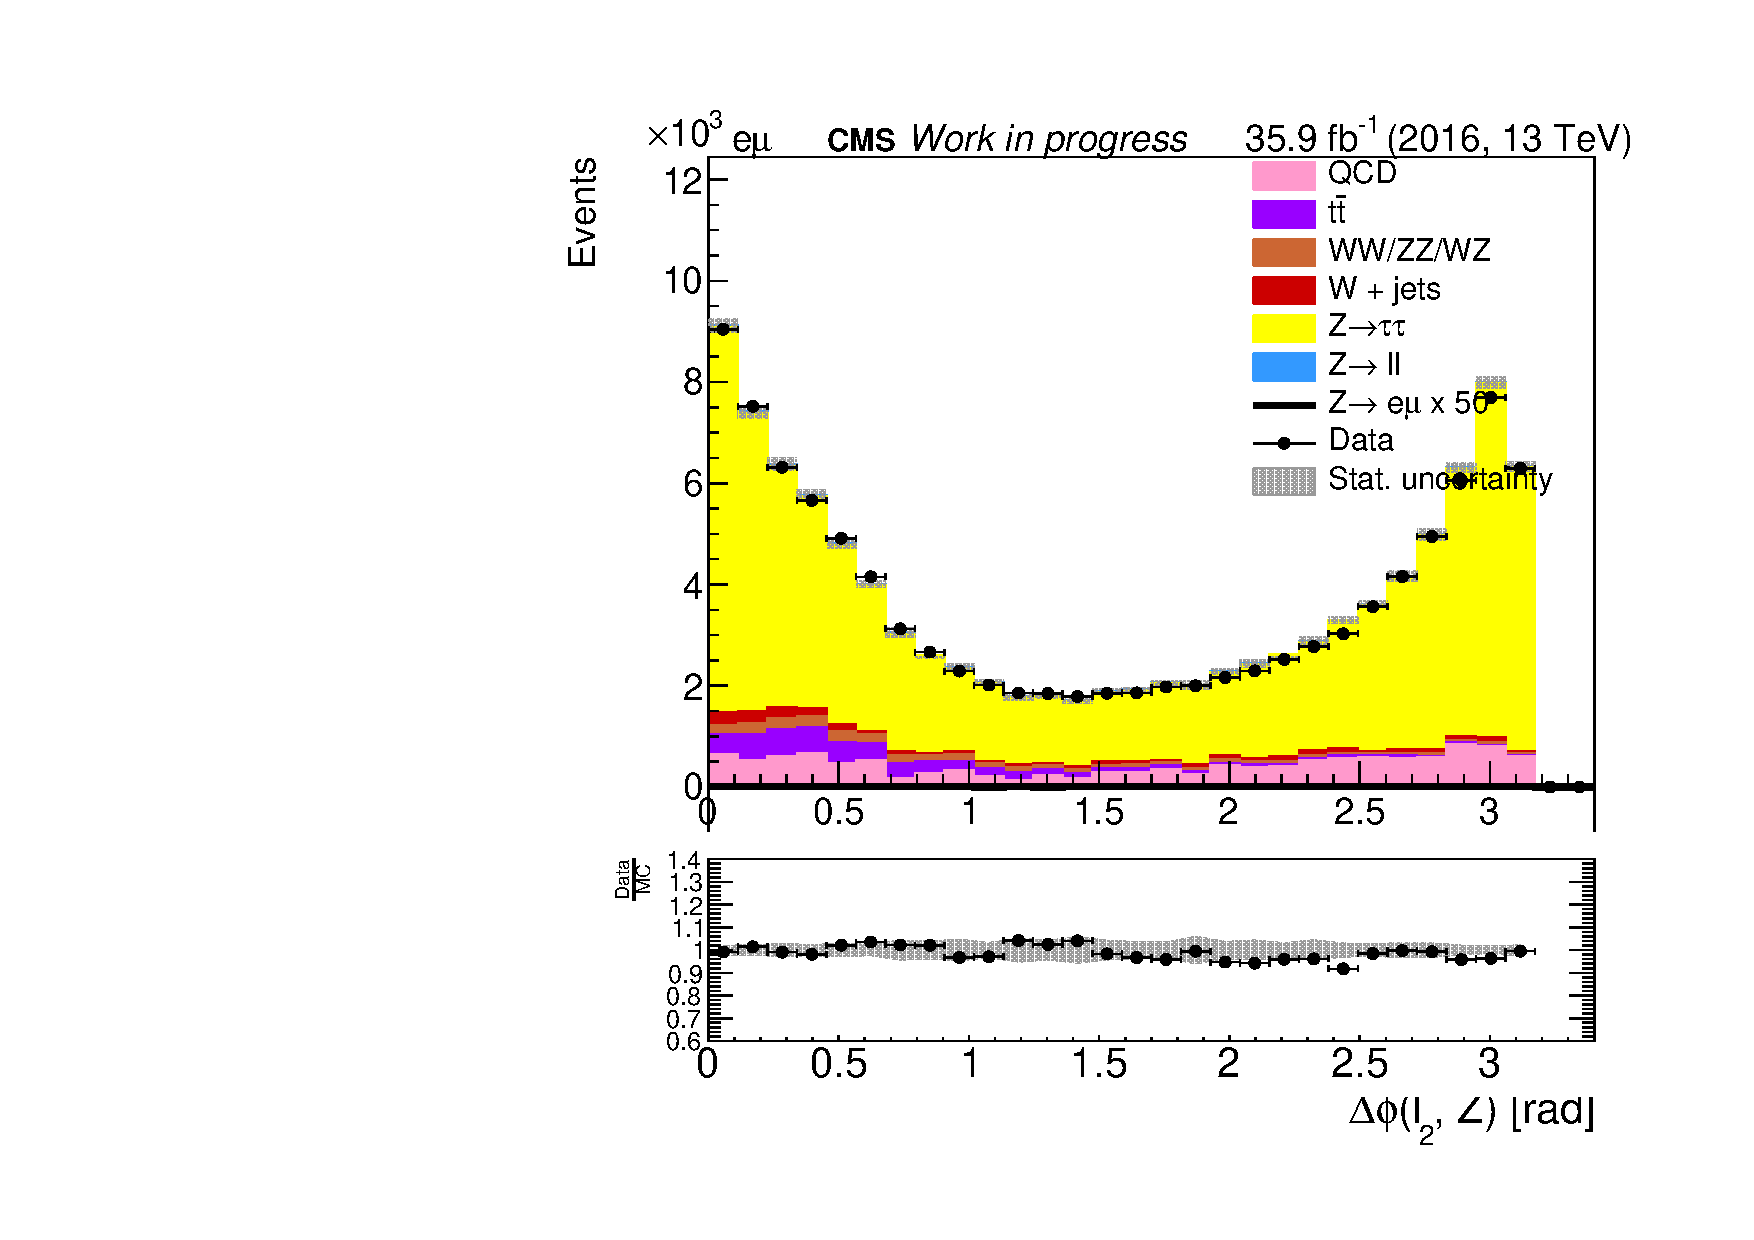
\includegraphics[width=0.45\textwidth]{plots/em/DeltaPhiL2Z_CR.pdf}
	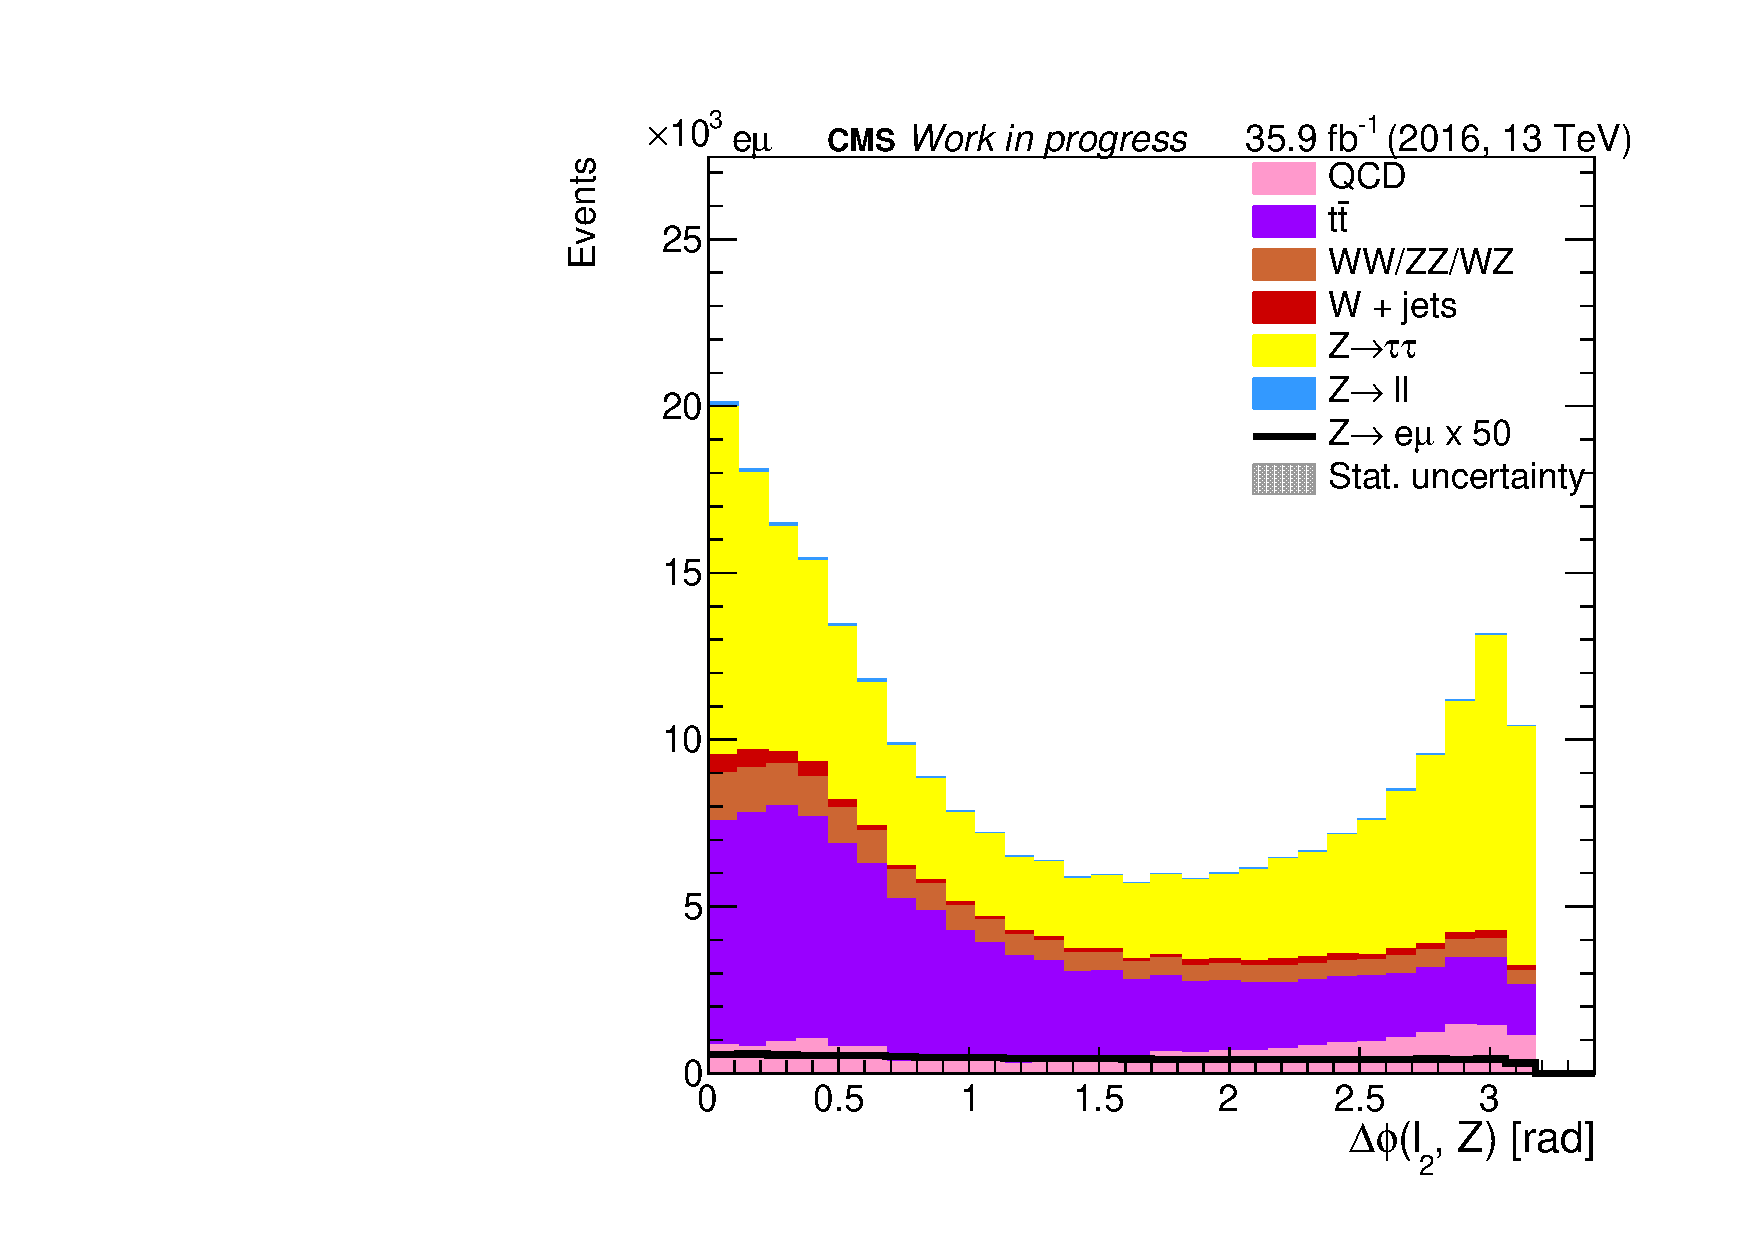
\includegraphics[width=0.45\textwidth]{plots/em/DeltaPhiL2Z_withsignal.pdf}

	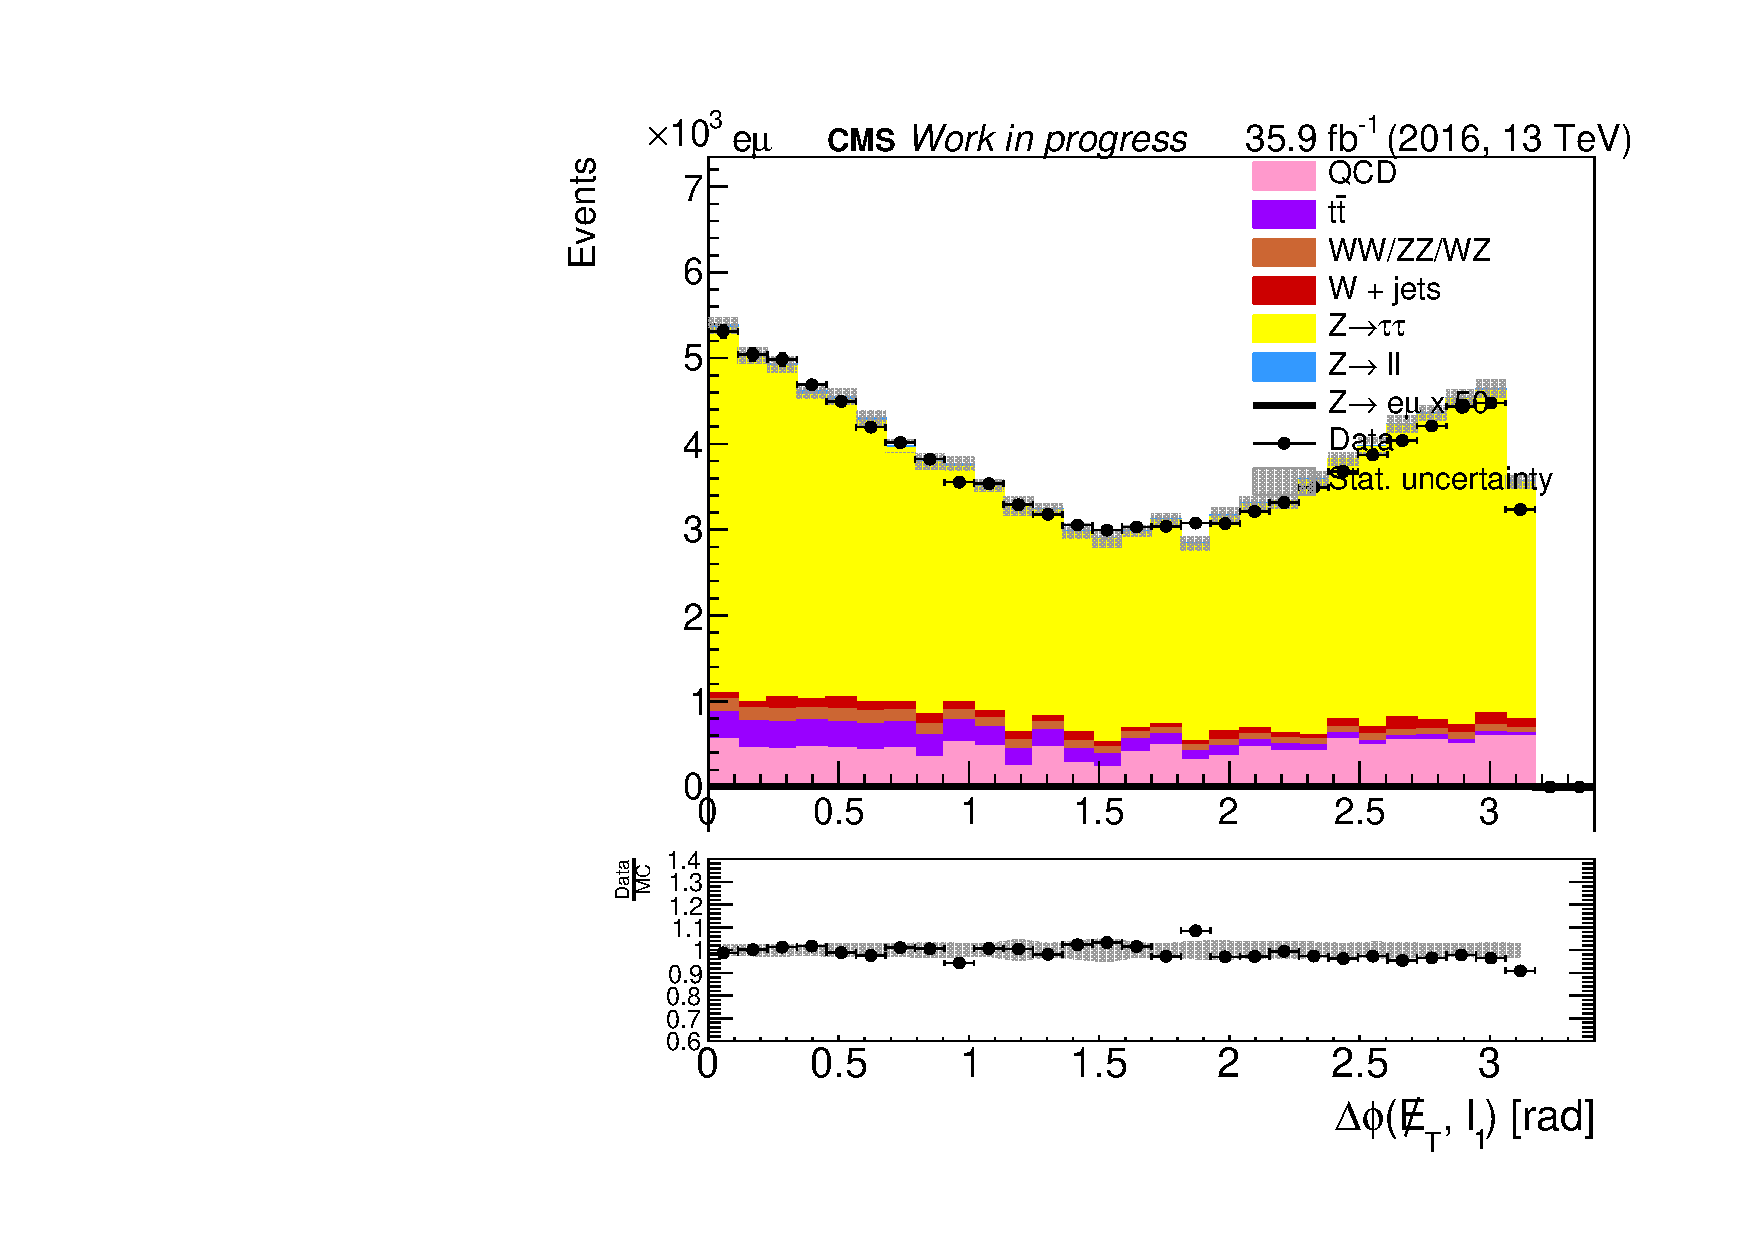
\includegraphics[width=0.45\textwidth]{plots/em/DeltaPhiMetL1_CR.pdf}
	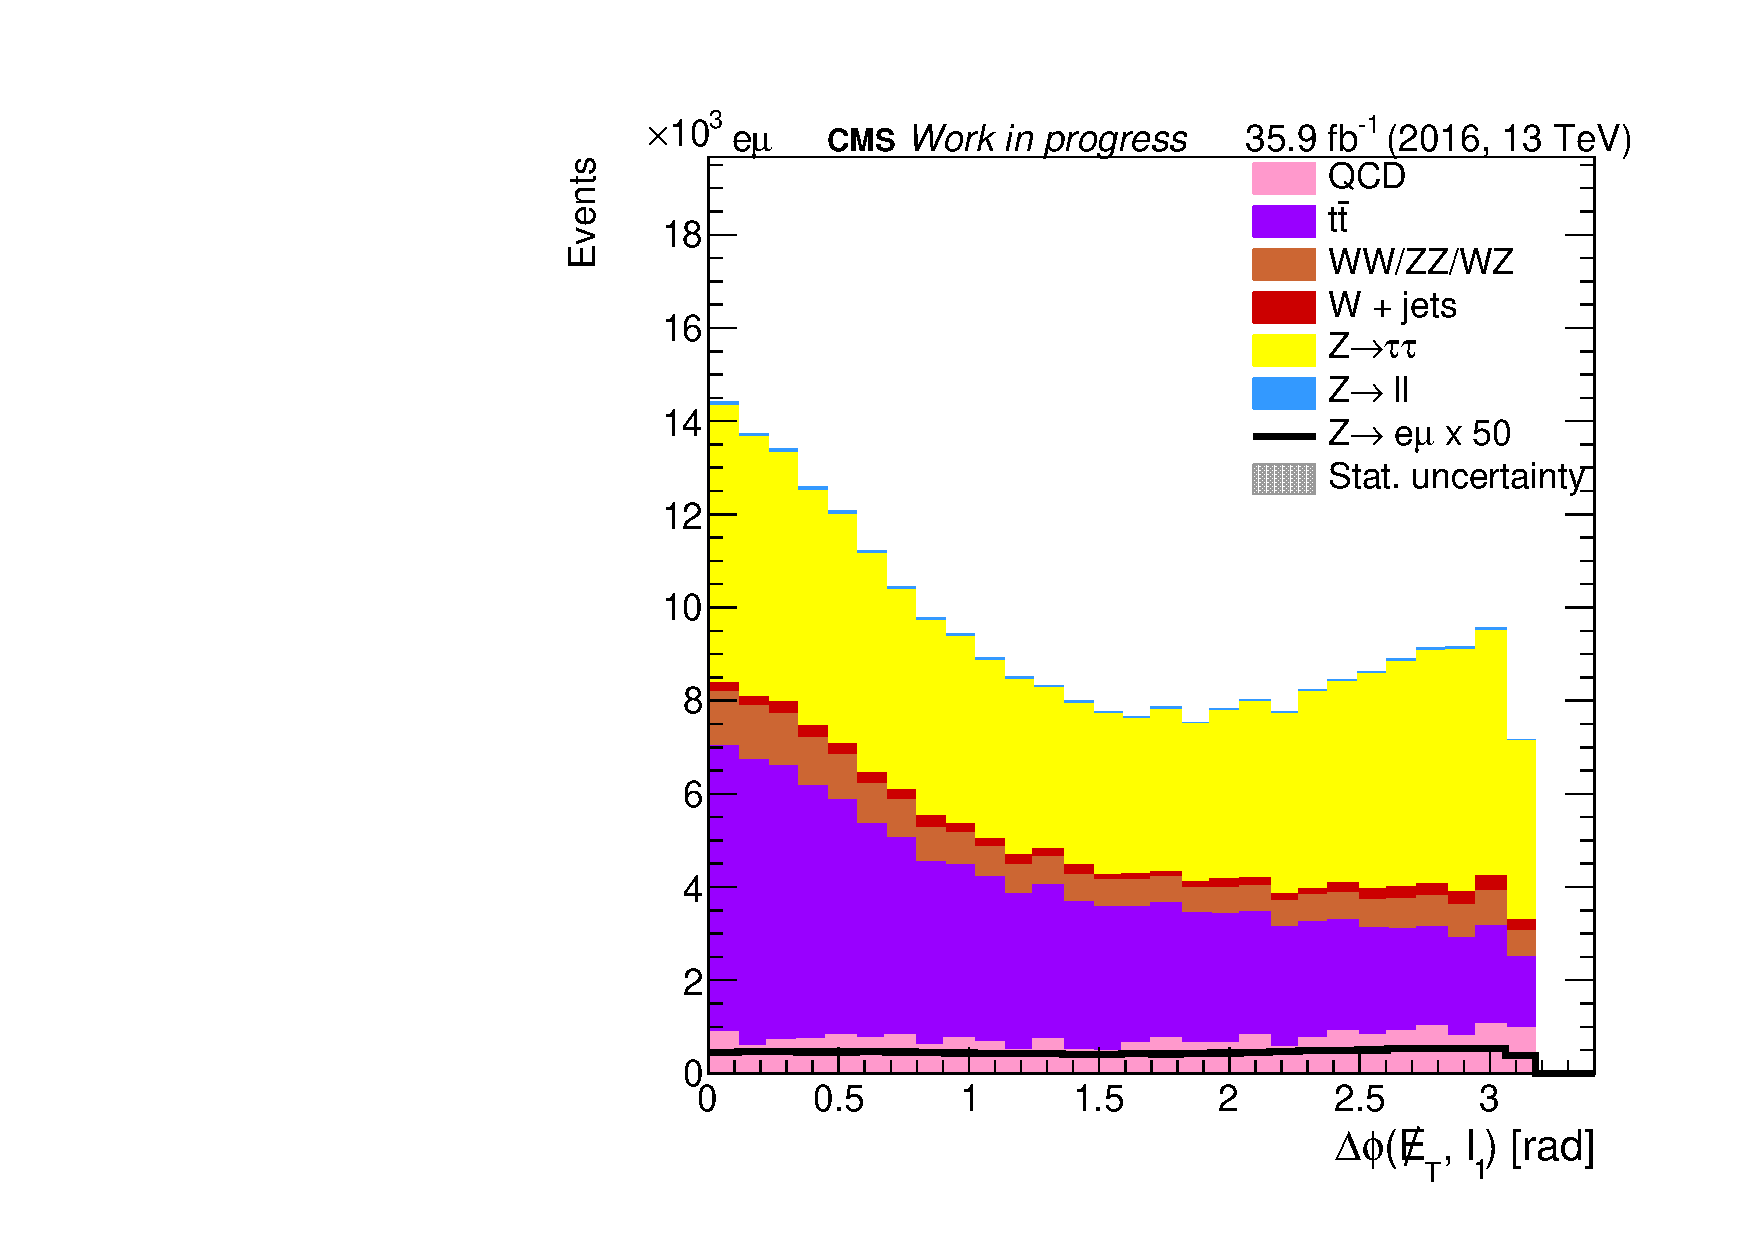
\includegraphics[width=0.45\textwidth]{plots/em/DeltaPhiMetL1_withsignal.pdf}

	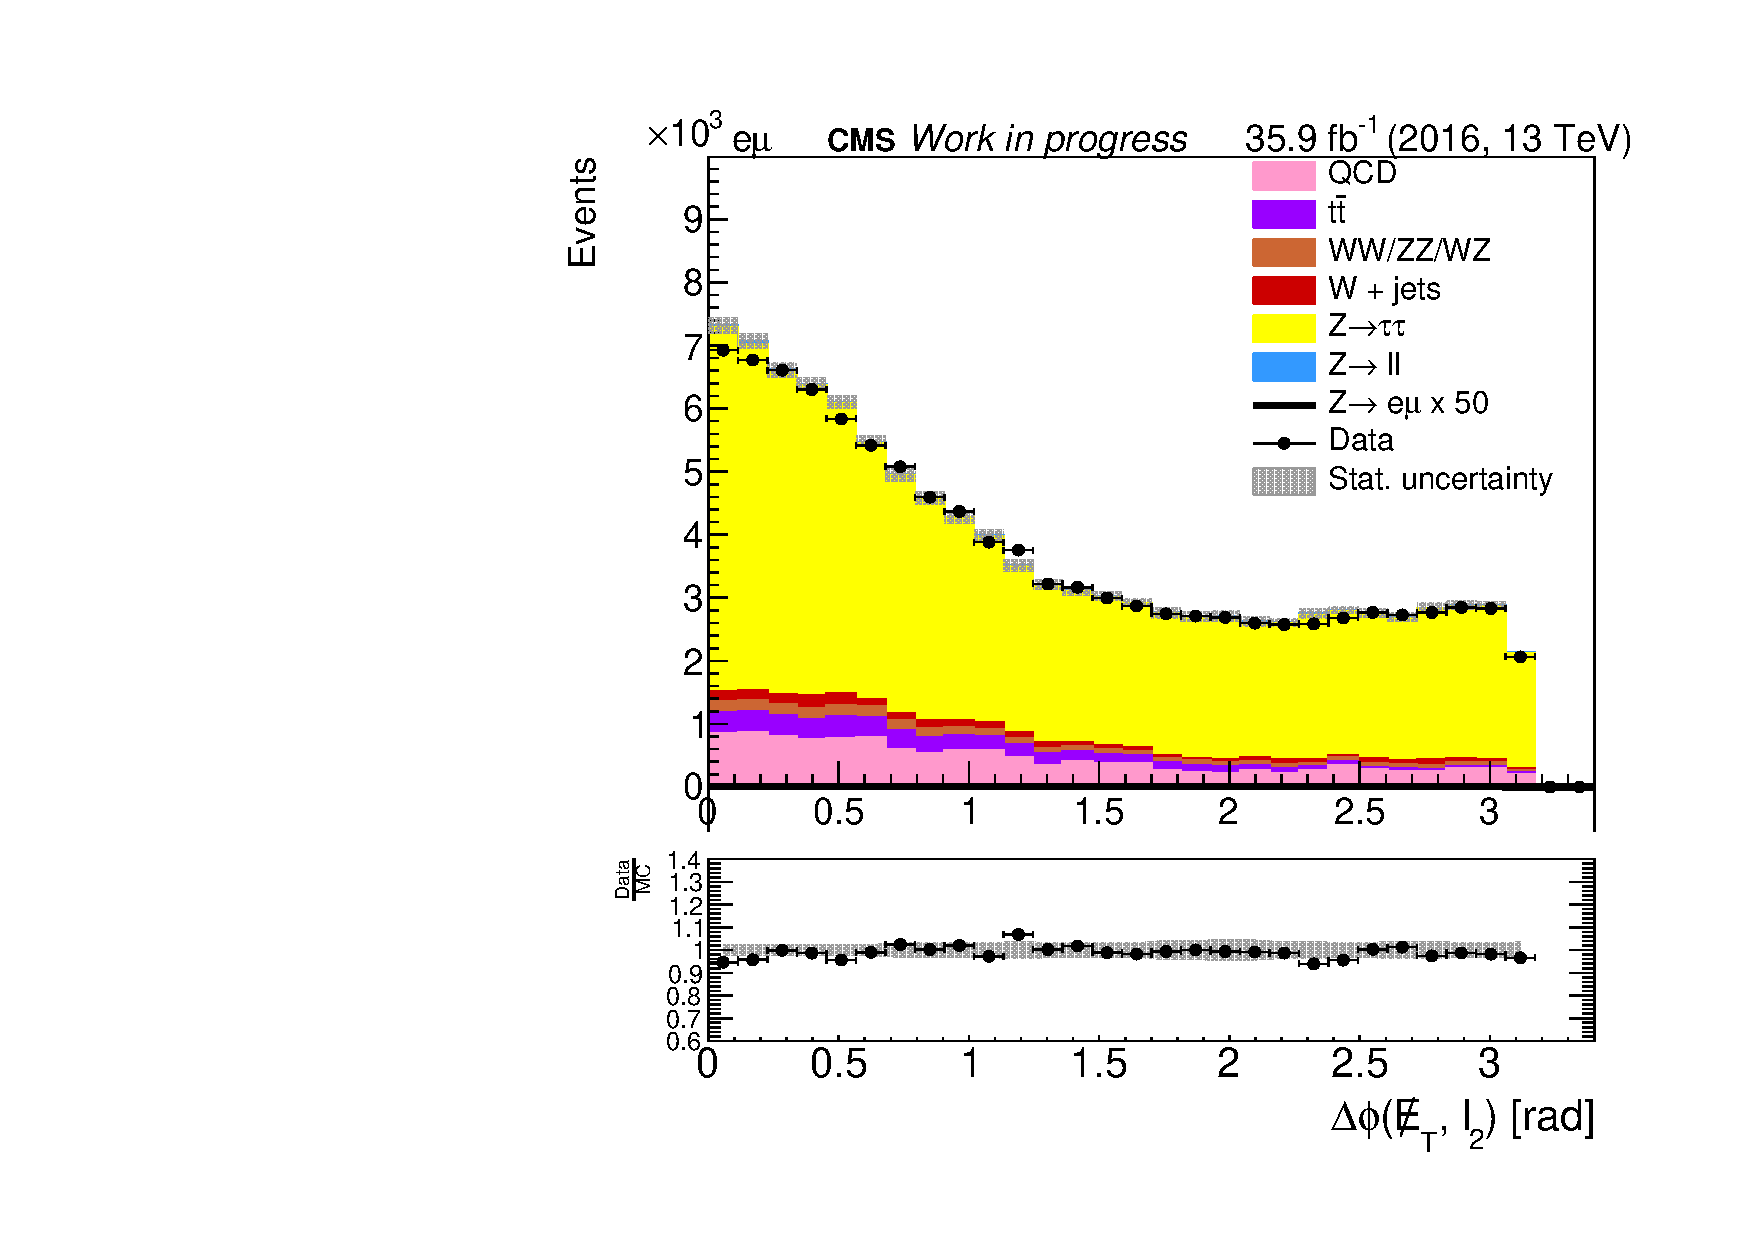
\includegraphics[width=0.45\textwidth]{plots/em/DeltaPhiMetL2_CR.pdf}
	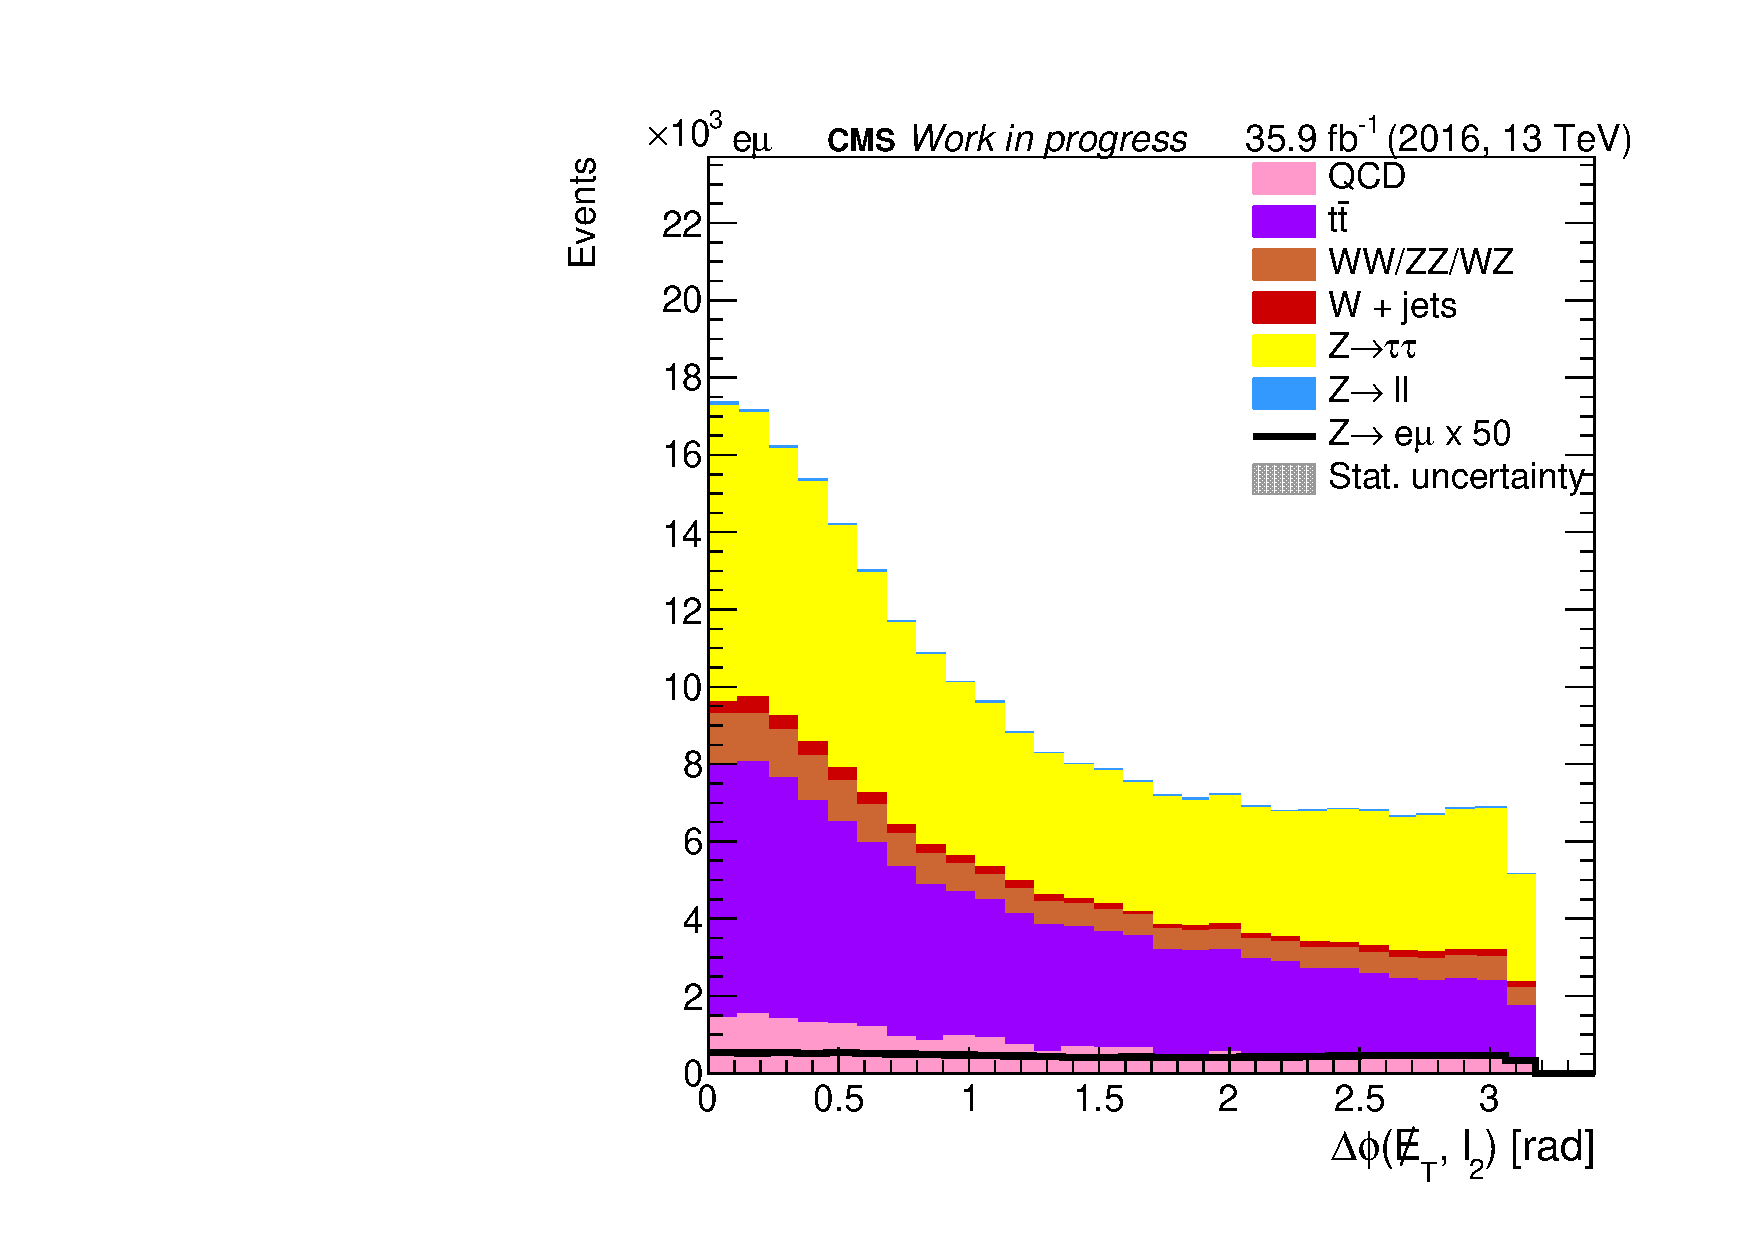
\includegraphics[width=0.45\textwidth]{plots/em/DeltaPhiMetL2_withsignal.pdf}
\end{figure}


\begin{figure}[htp]
	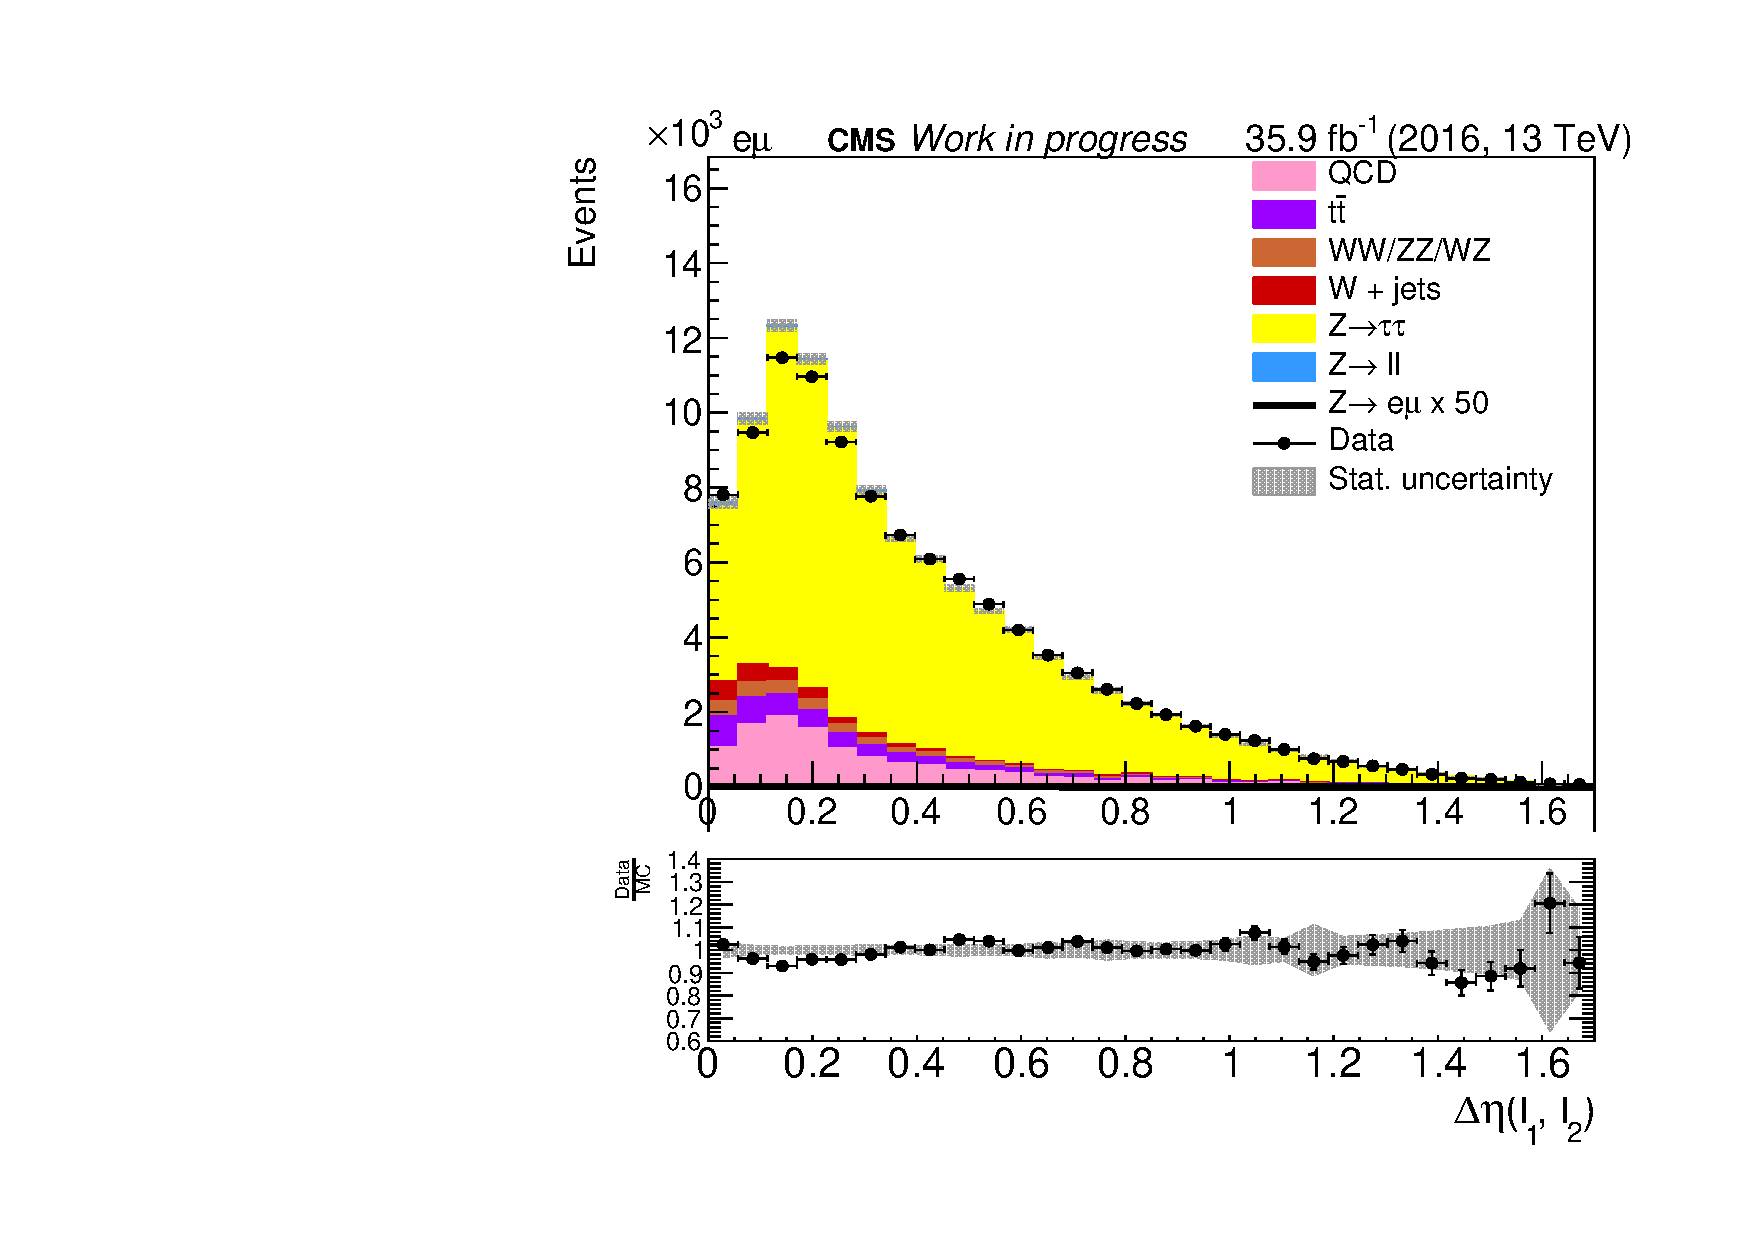
\includegraphics[width=0.45\textwidth]{plots/em/DiEta_CR.pdf}
	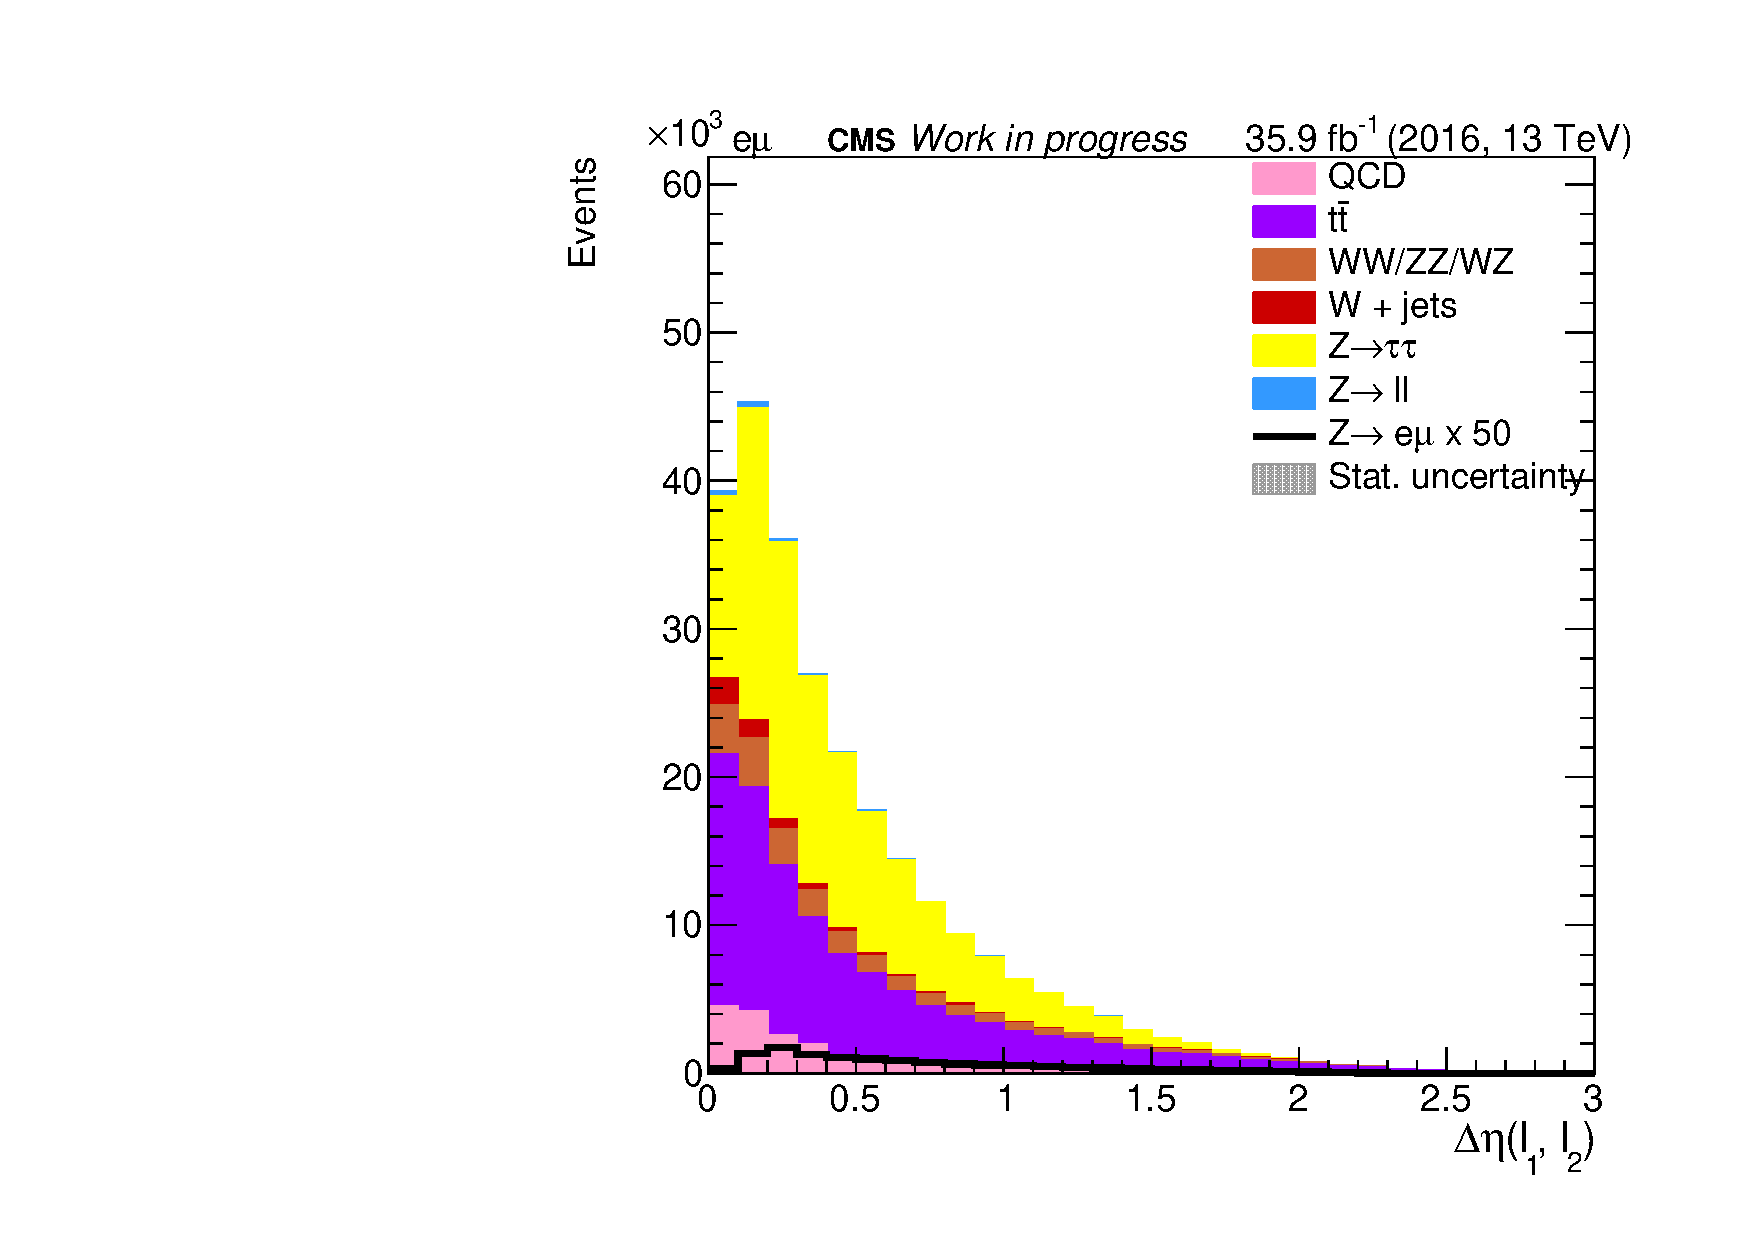
\includegraphics[width=0.45\textwidth]{plots/em/DiEta_withsignal.pdf}

	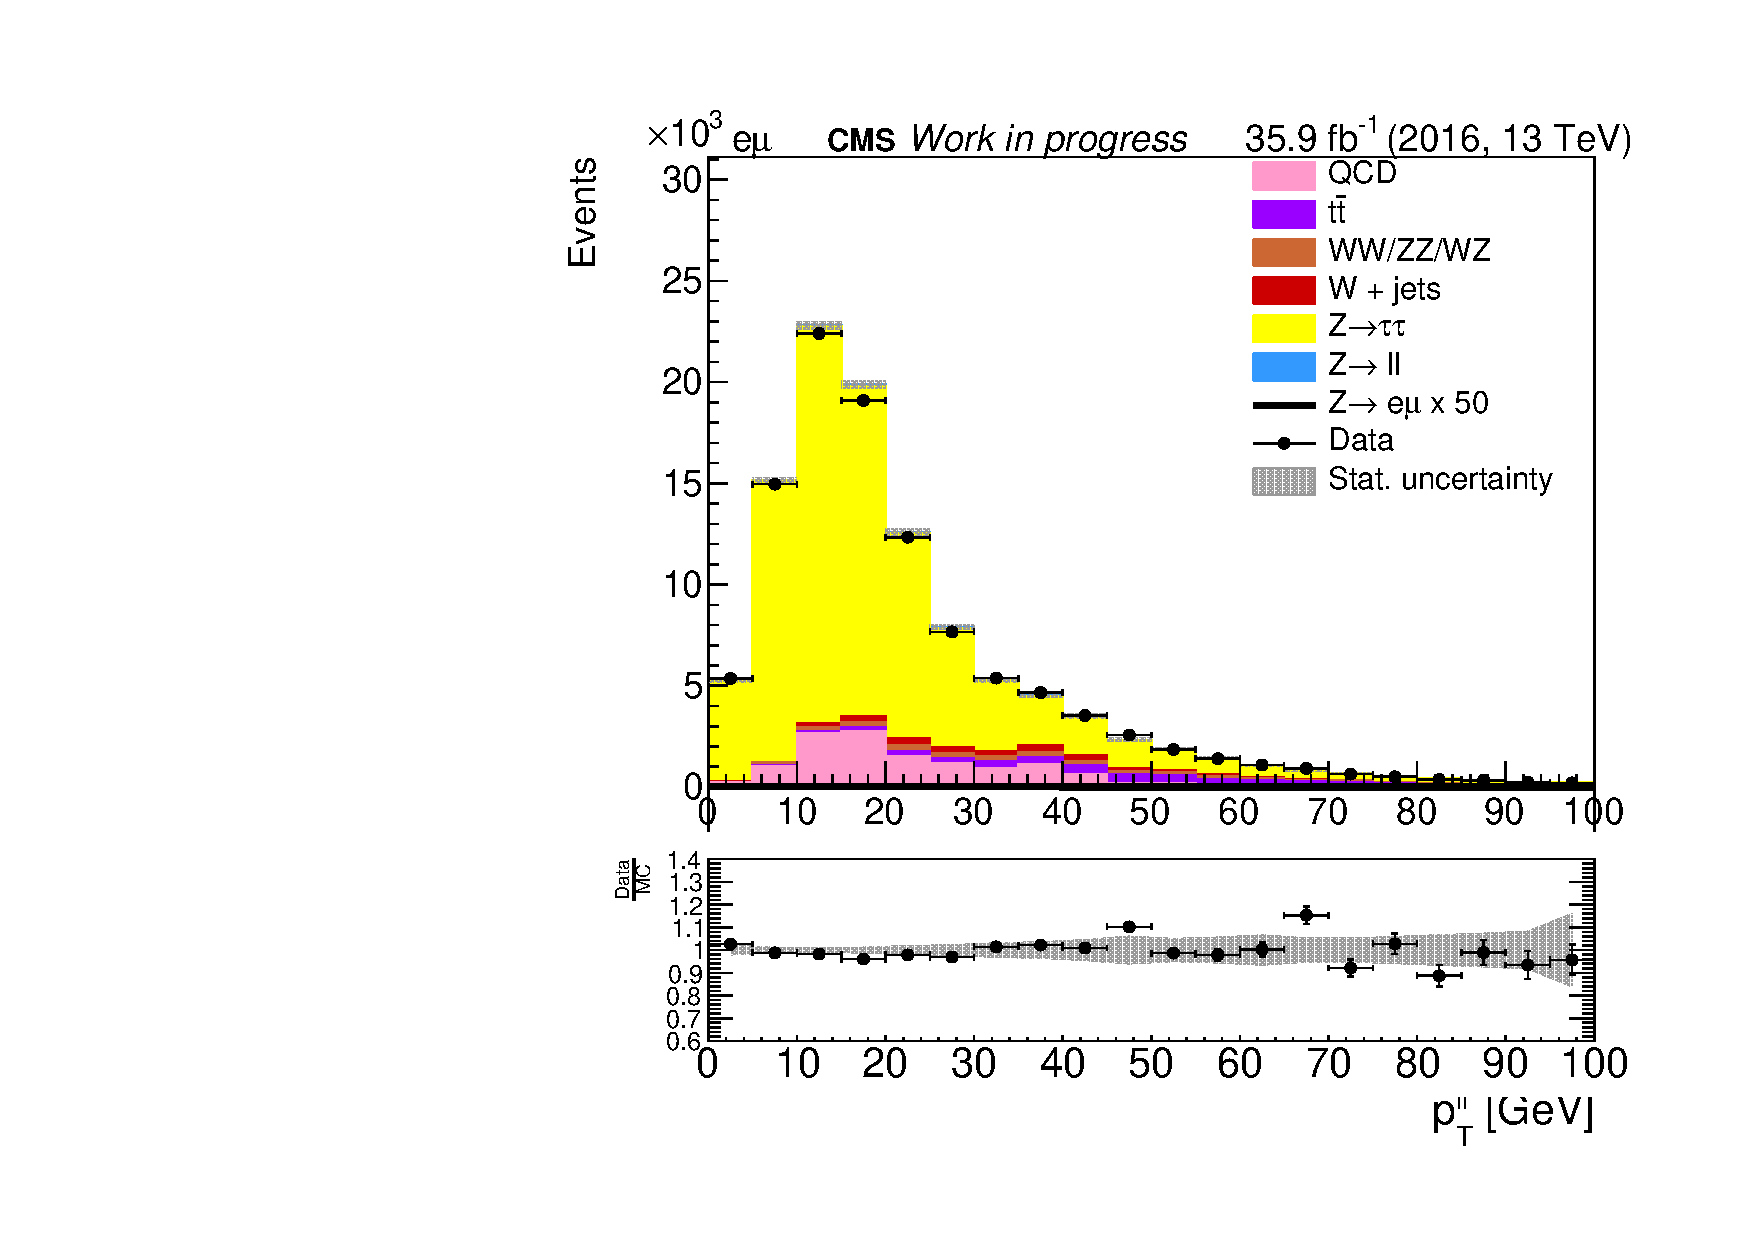
\includegraphics[width=0.45\textwidth]{plots/em/DiLepPt_CR.pdf}
	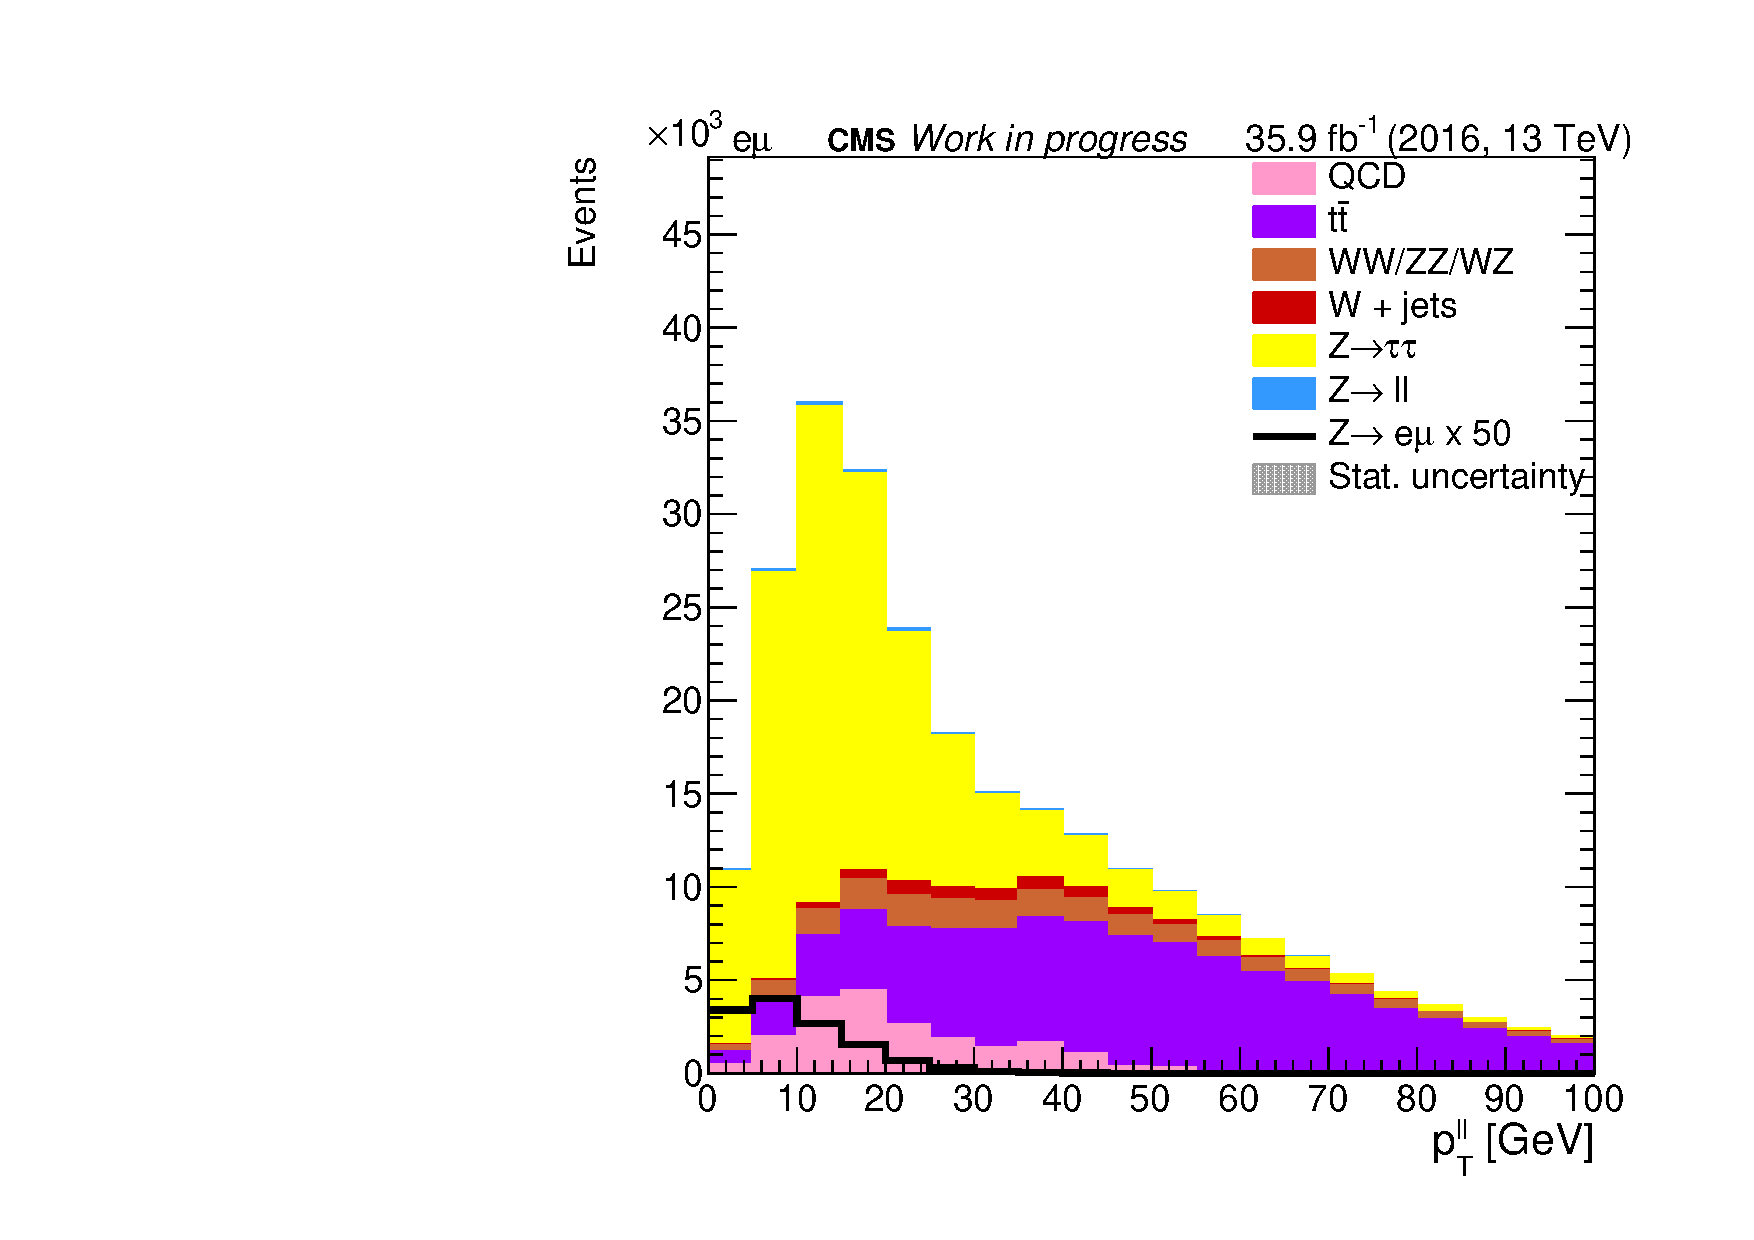
\includegraphics[width=0.45\textwidth]{plots/em/DiLepPt_withsignal.pdf}

	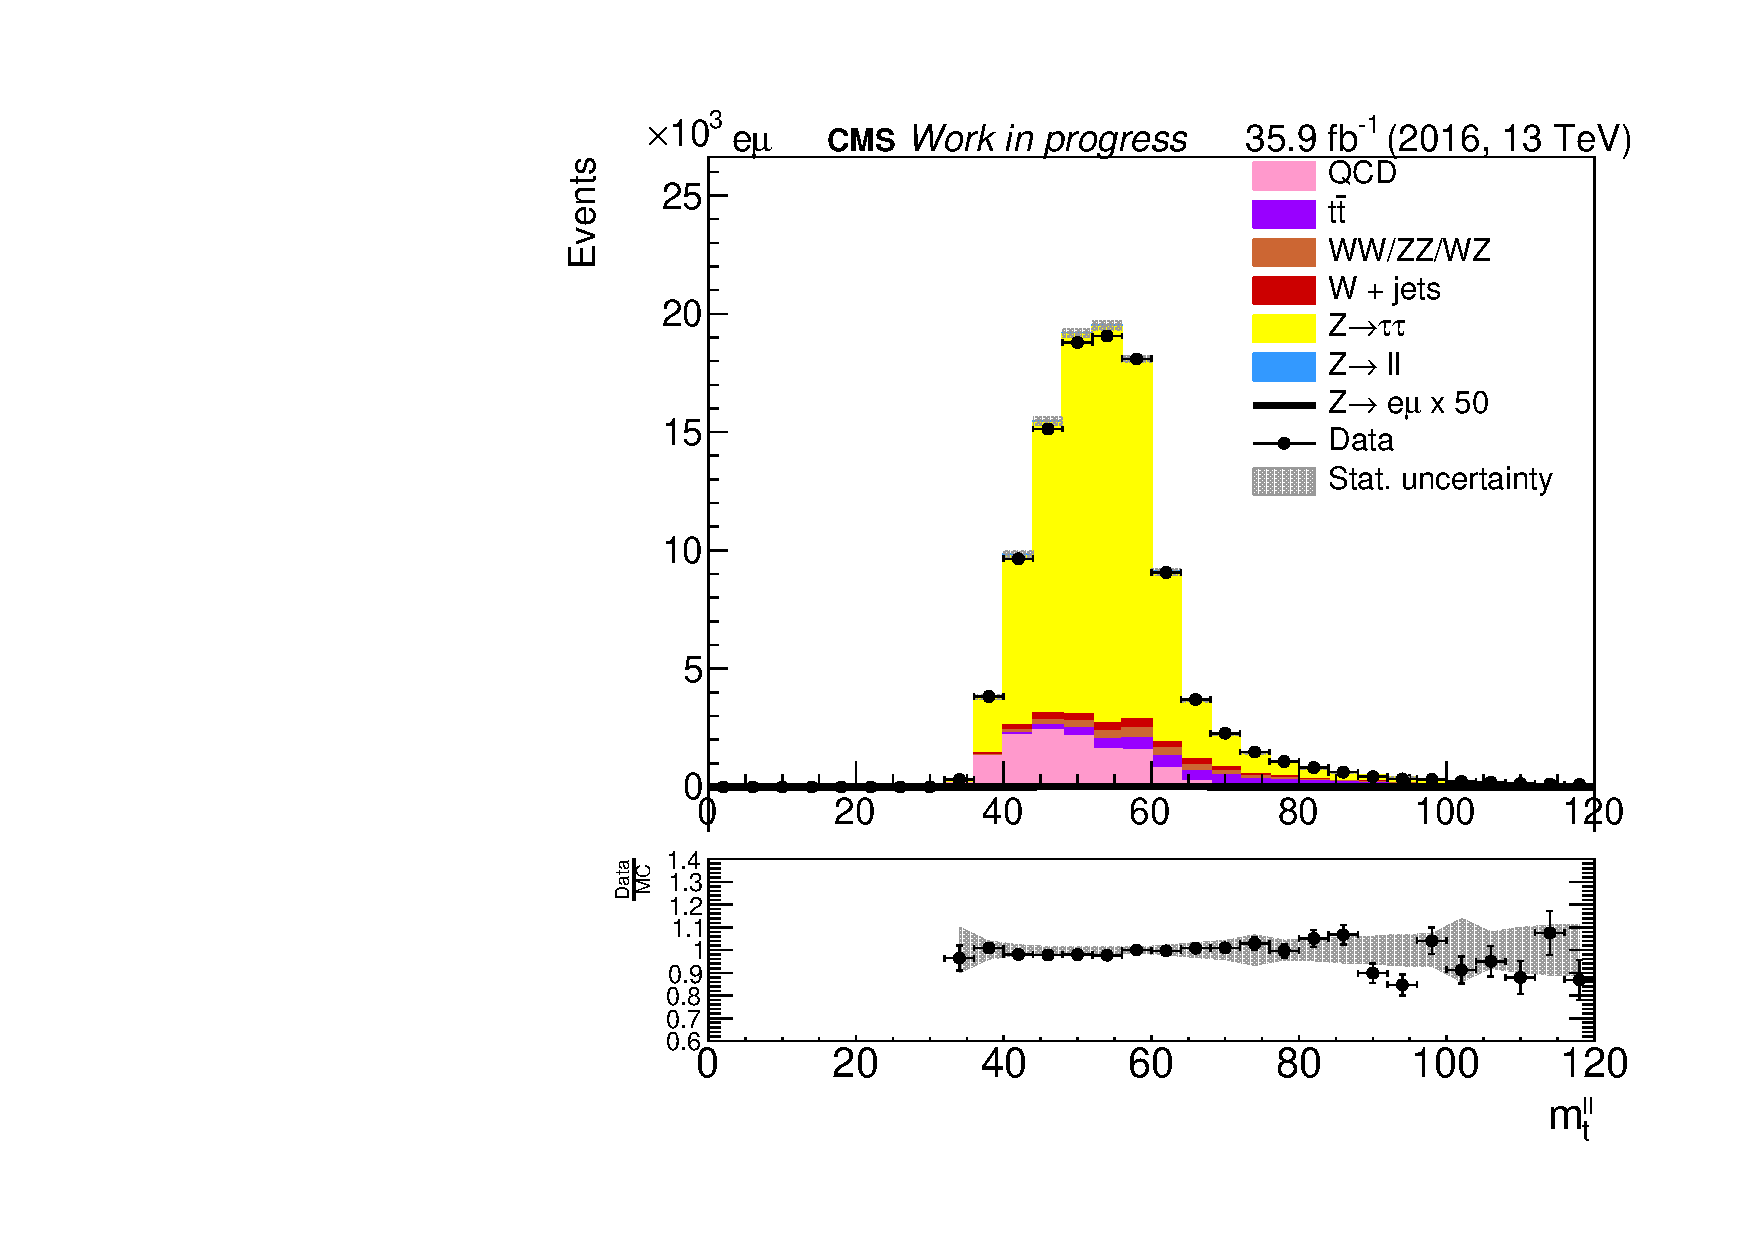
\includegraphics[width=0.45\textwidth]{plots/em/DiTransverseMass_CR.pdf}
	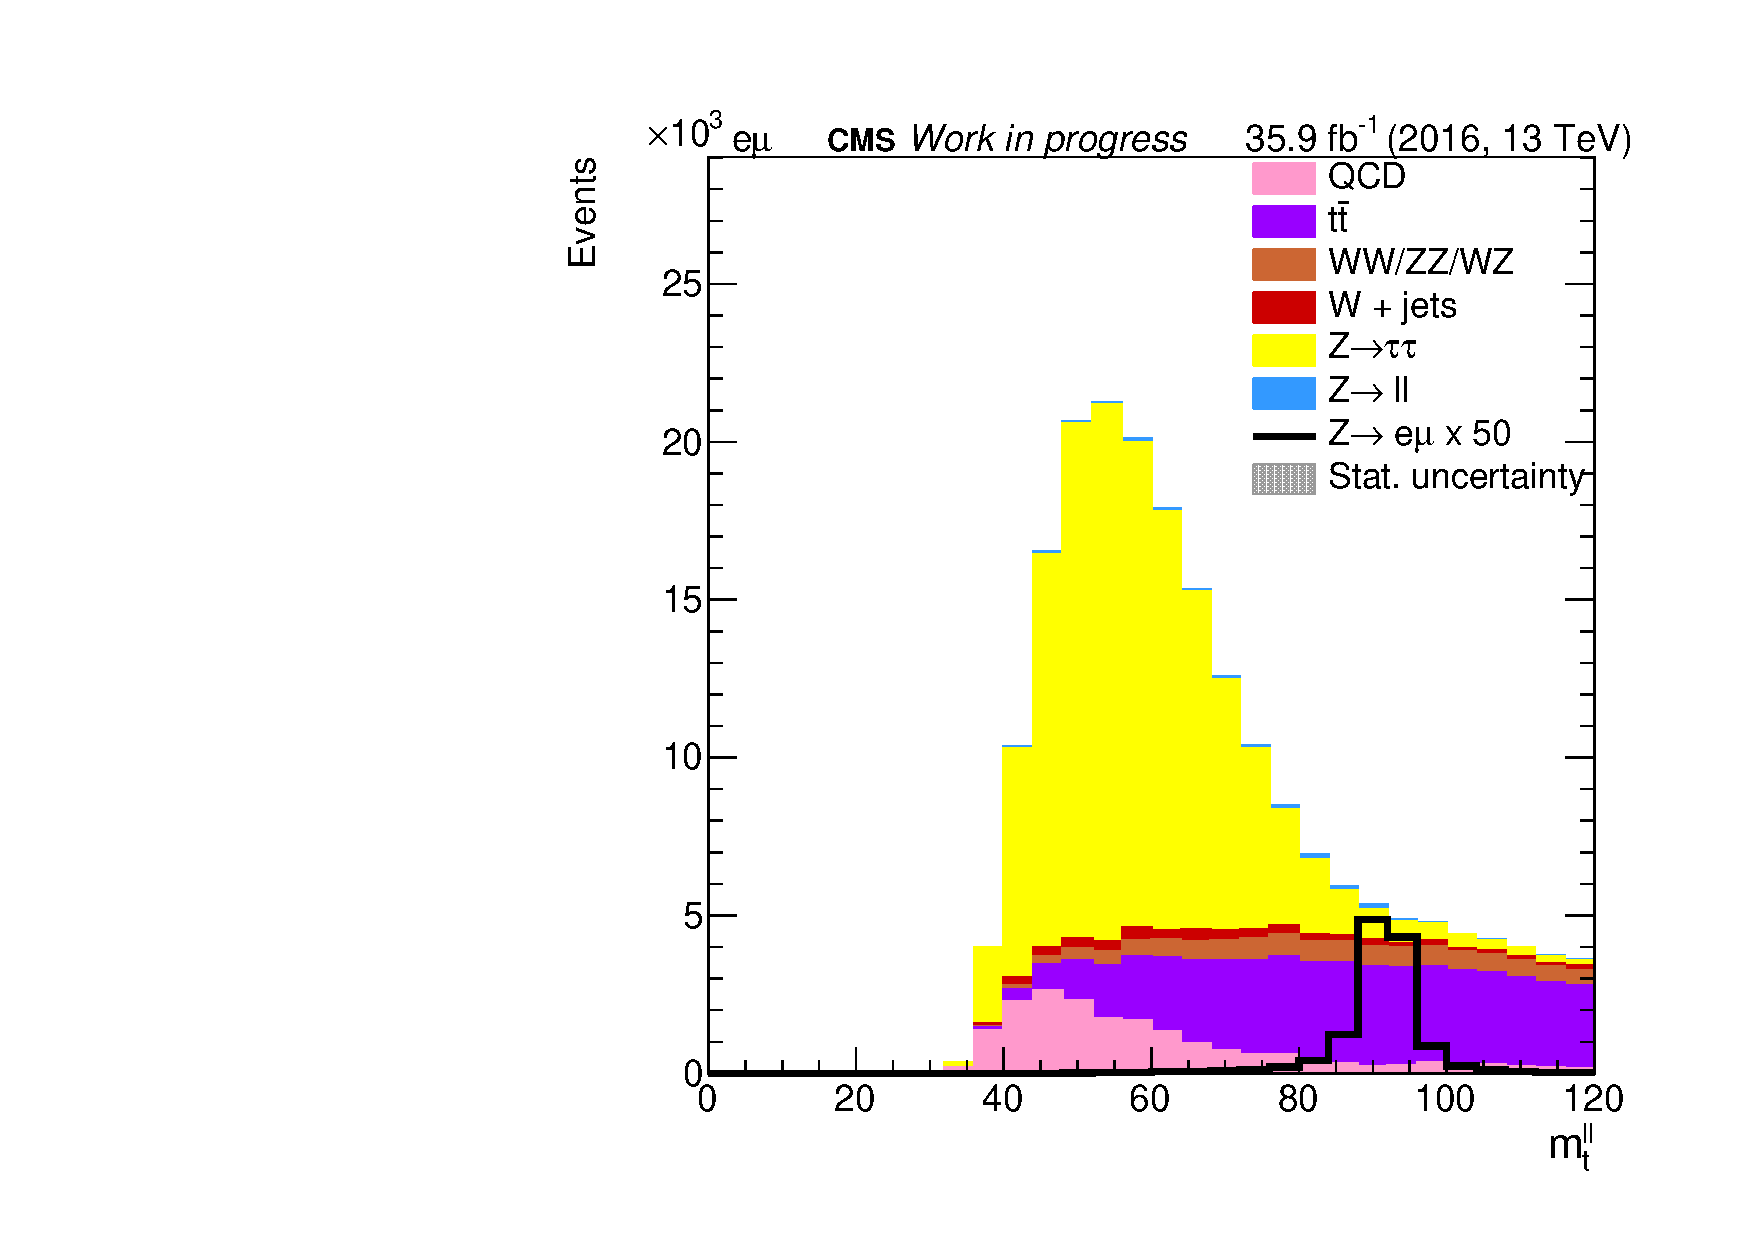
\includegraphics[width=0.45\textwidth]{plots/em/DiTransverseMass_withsignal.pdf}
\end{figure}


\begin{figure}[htp]
	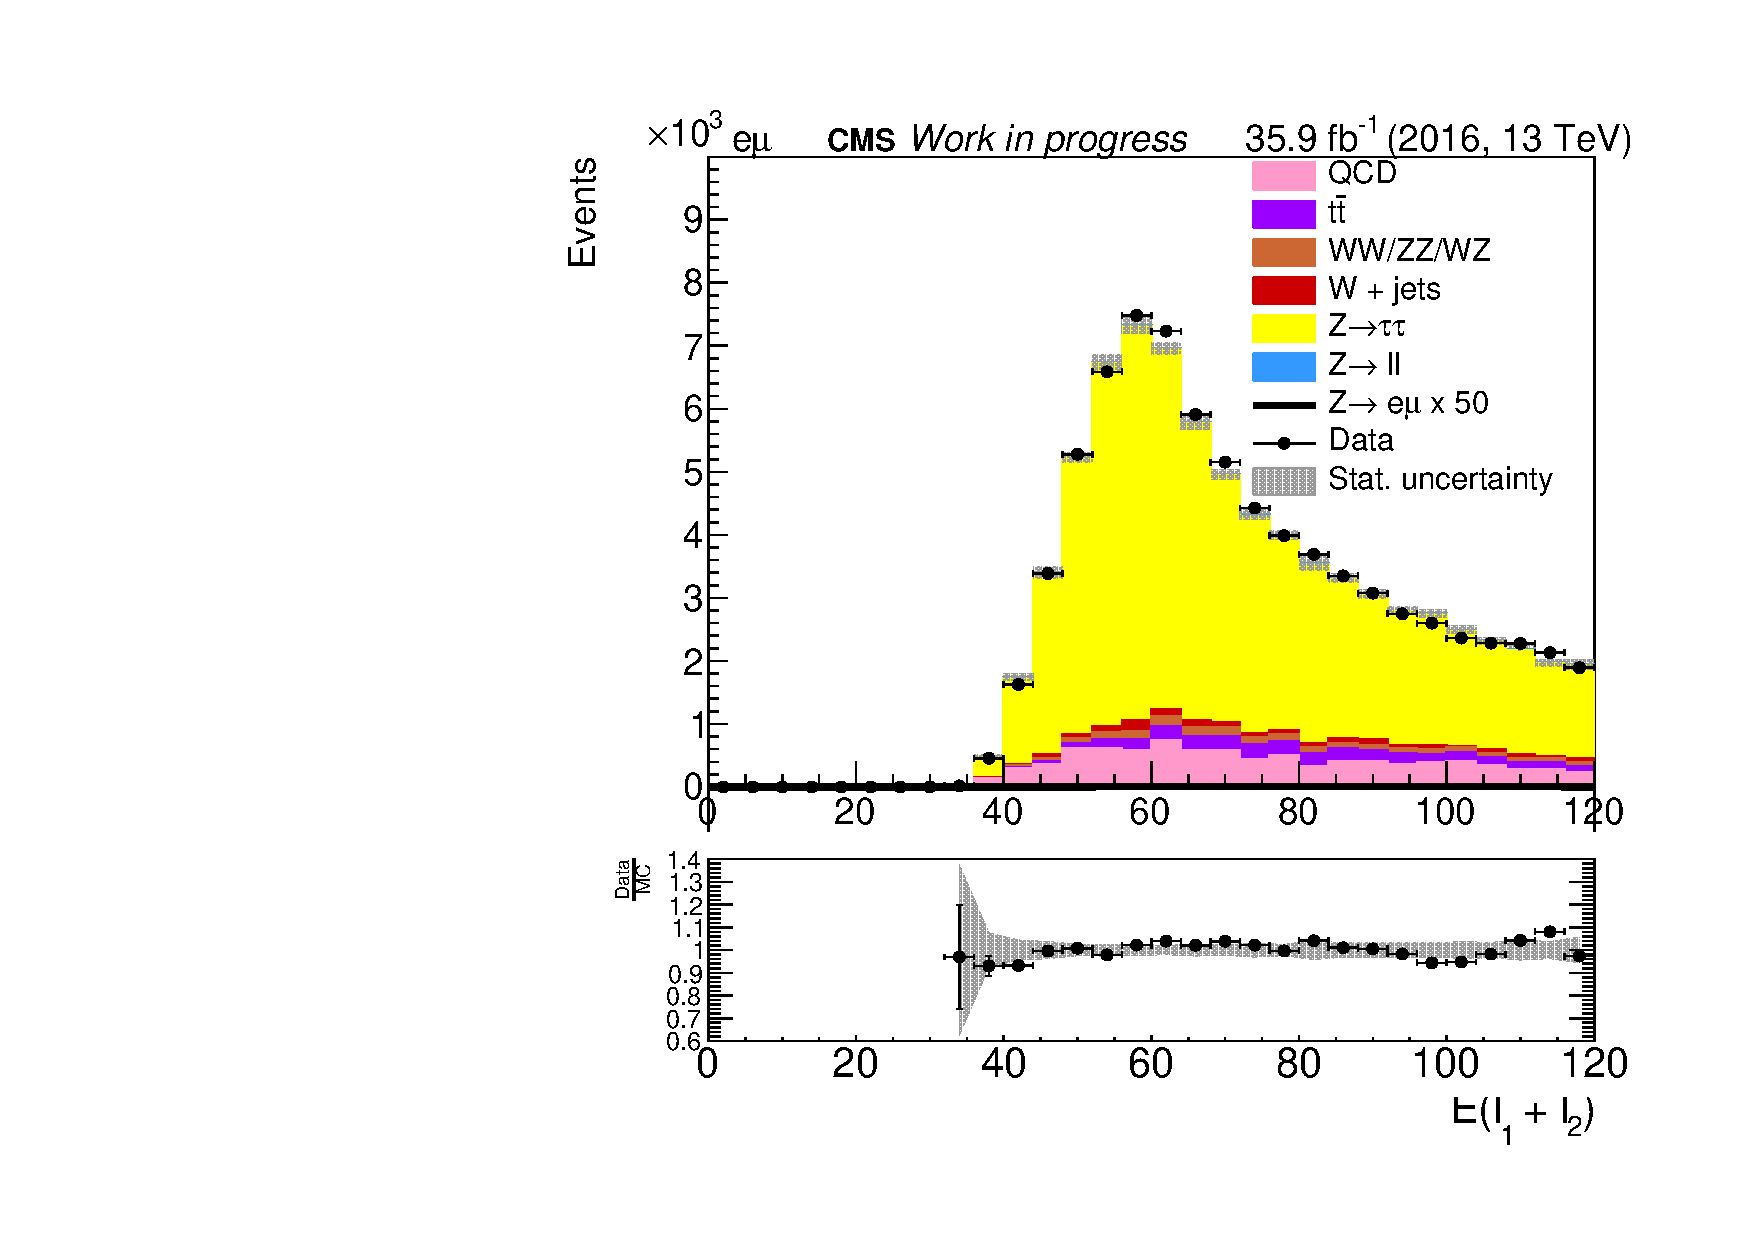
\includegraphics[width=0.45\textwidth]{plots/em/EnergySum_CR.pdf}
	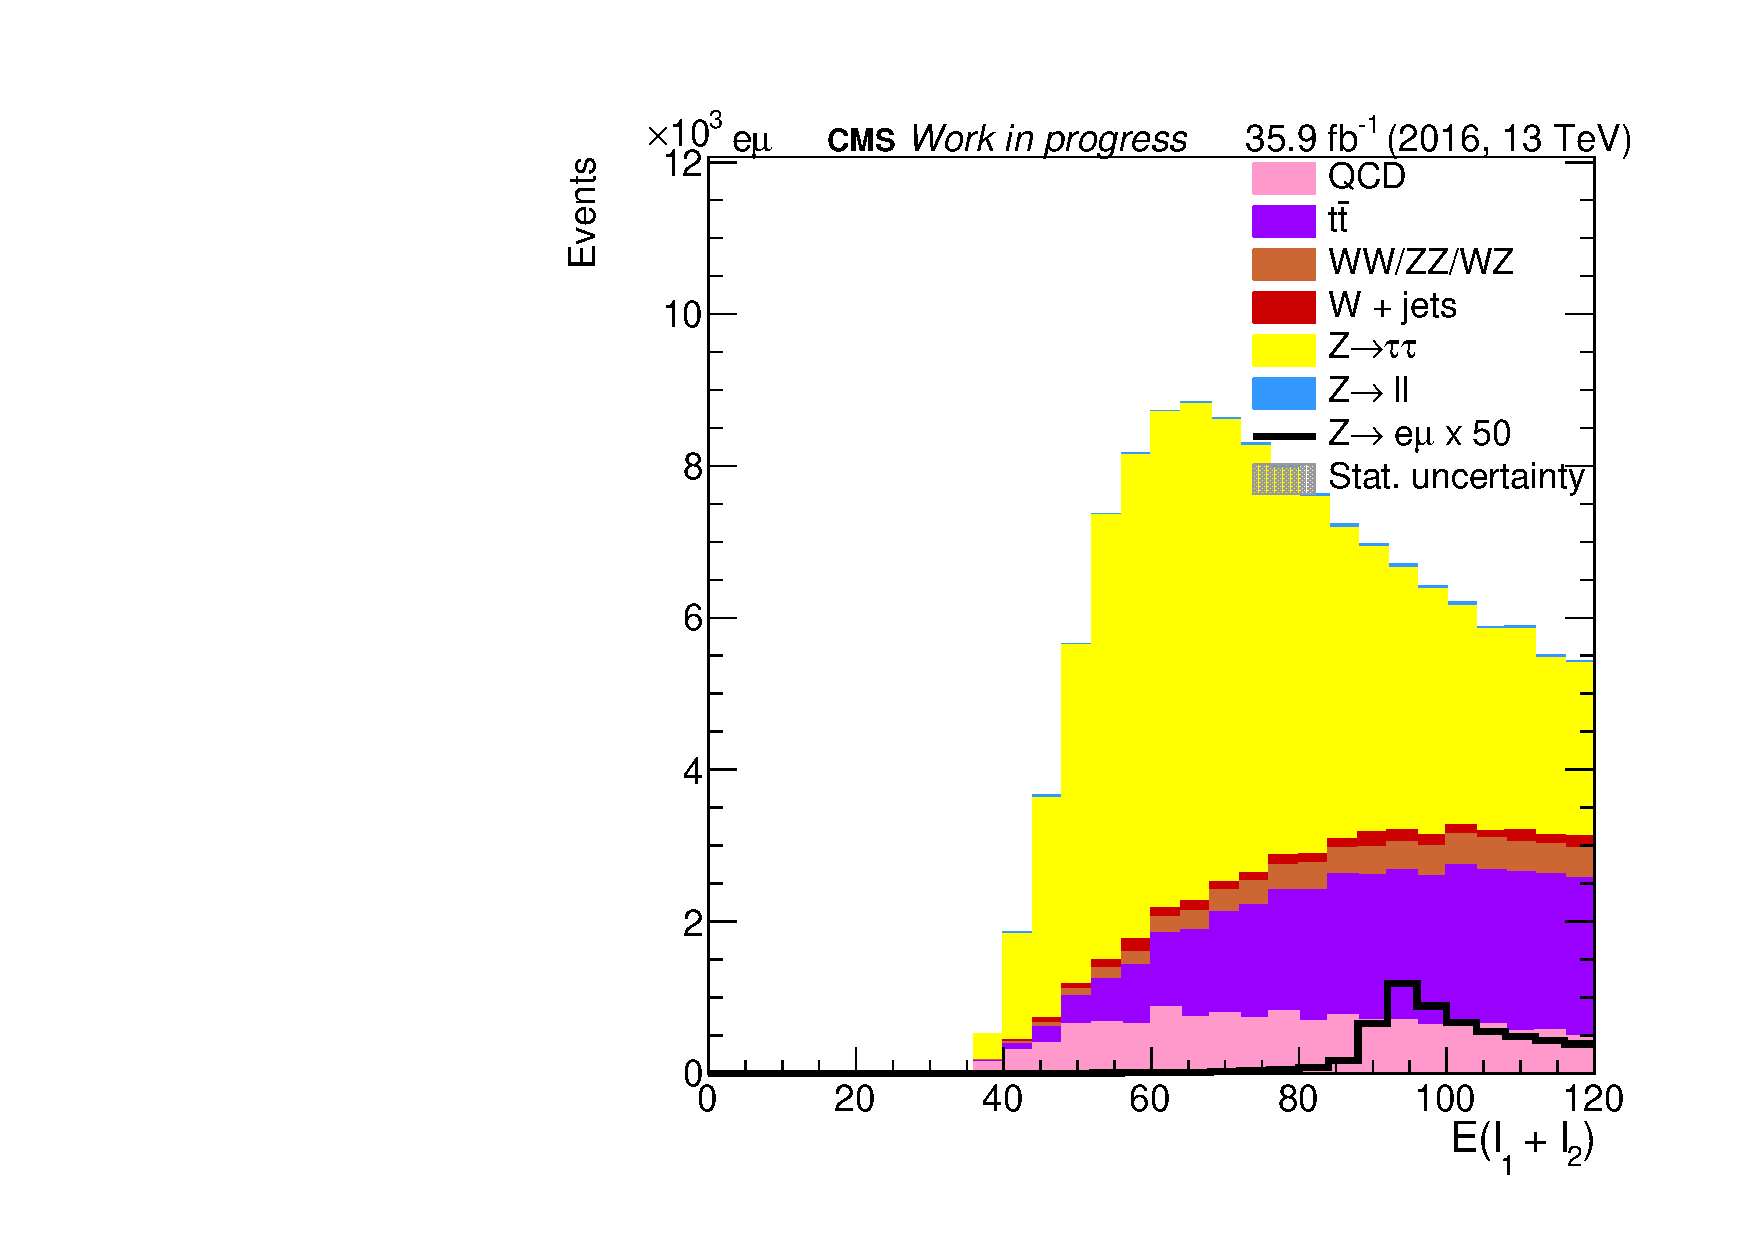
\includegraphics[width=0.45\textwidth]{plots/em/EnergySum_withsignal.pdf}

	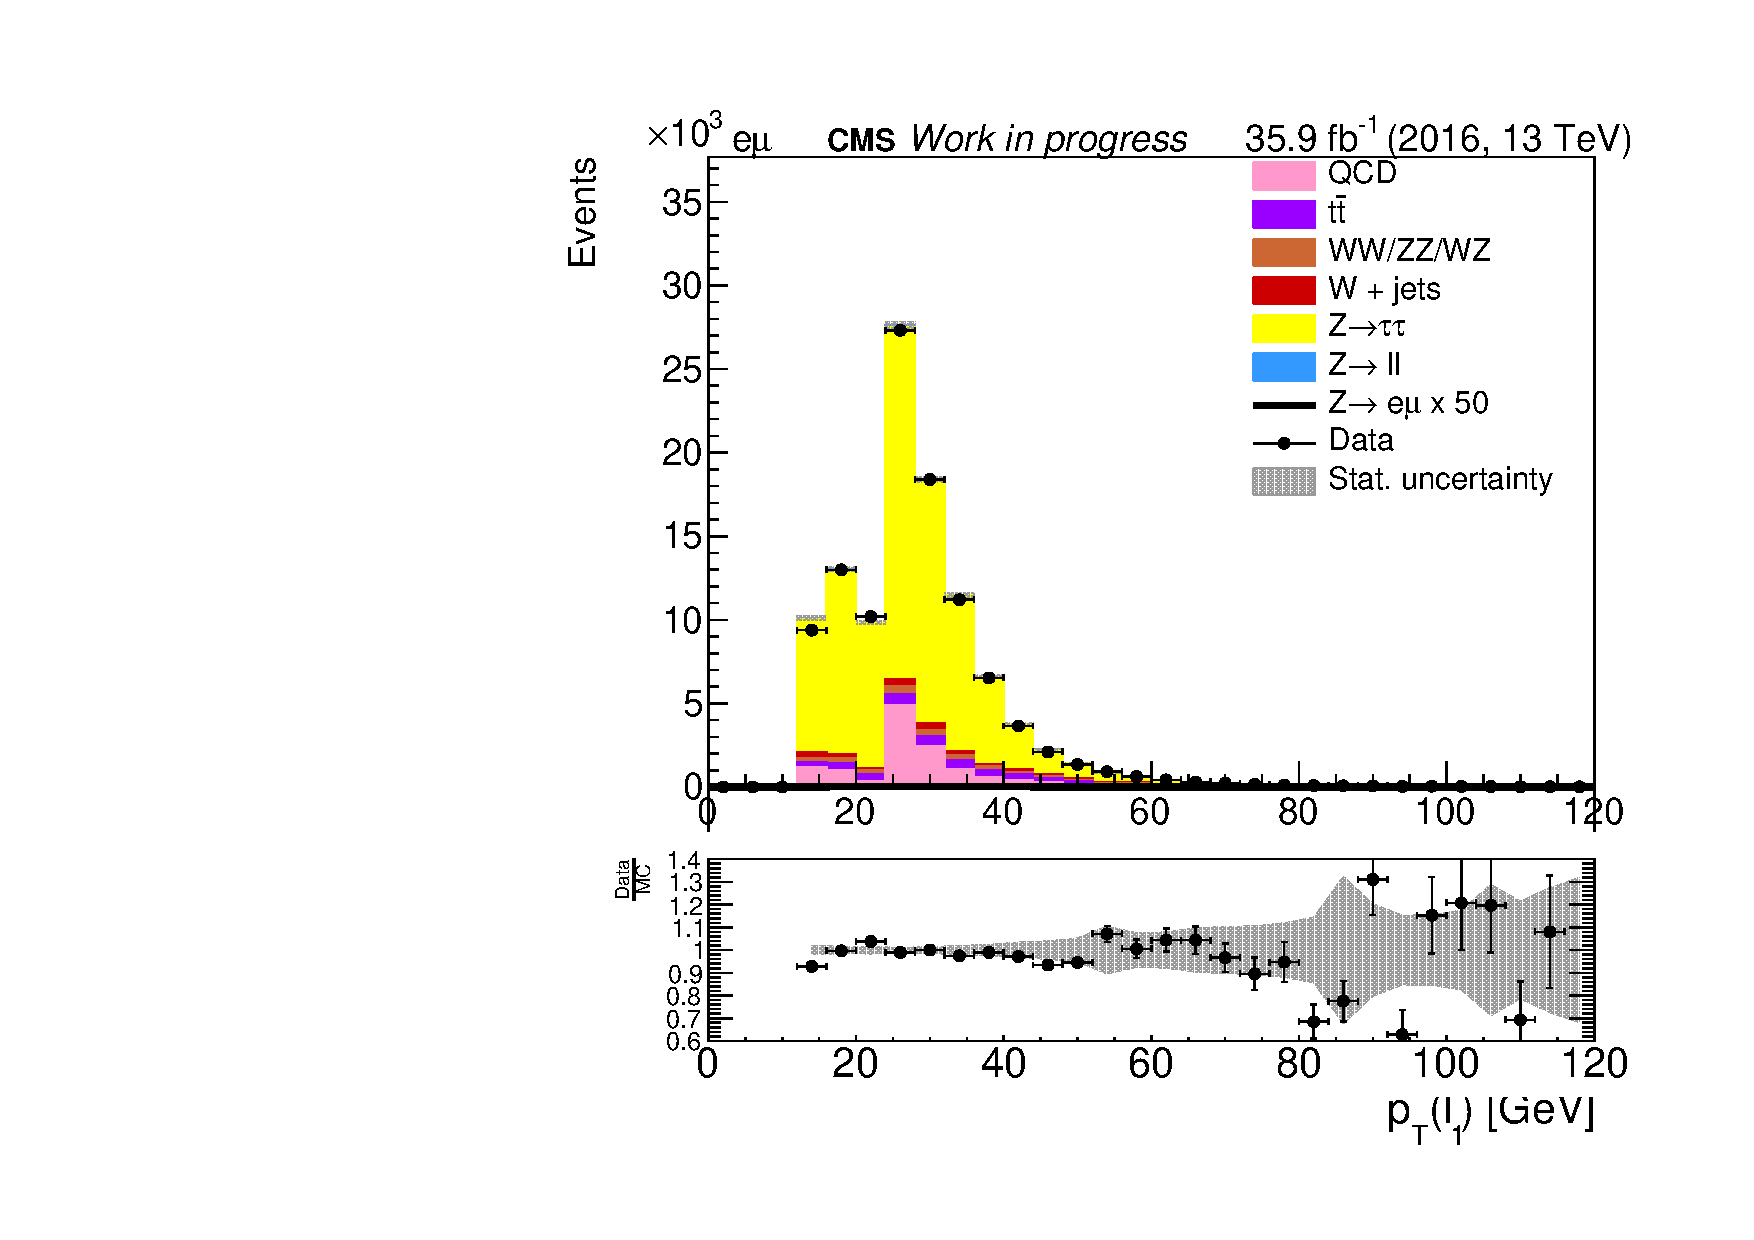
\includegraphics[width=0.45\textwidth]{plots/em/TransverseMomentum1_CR.pdf}
	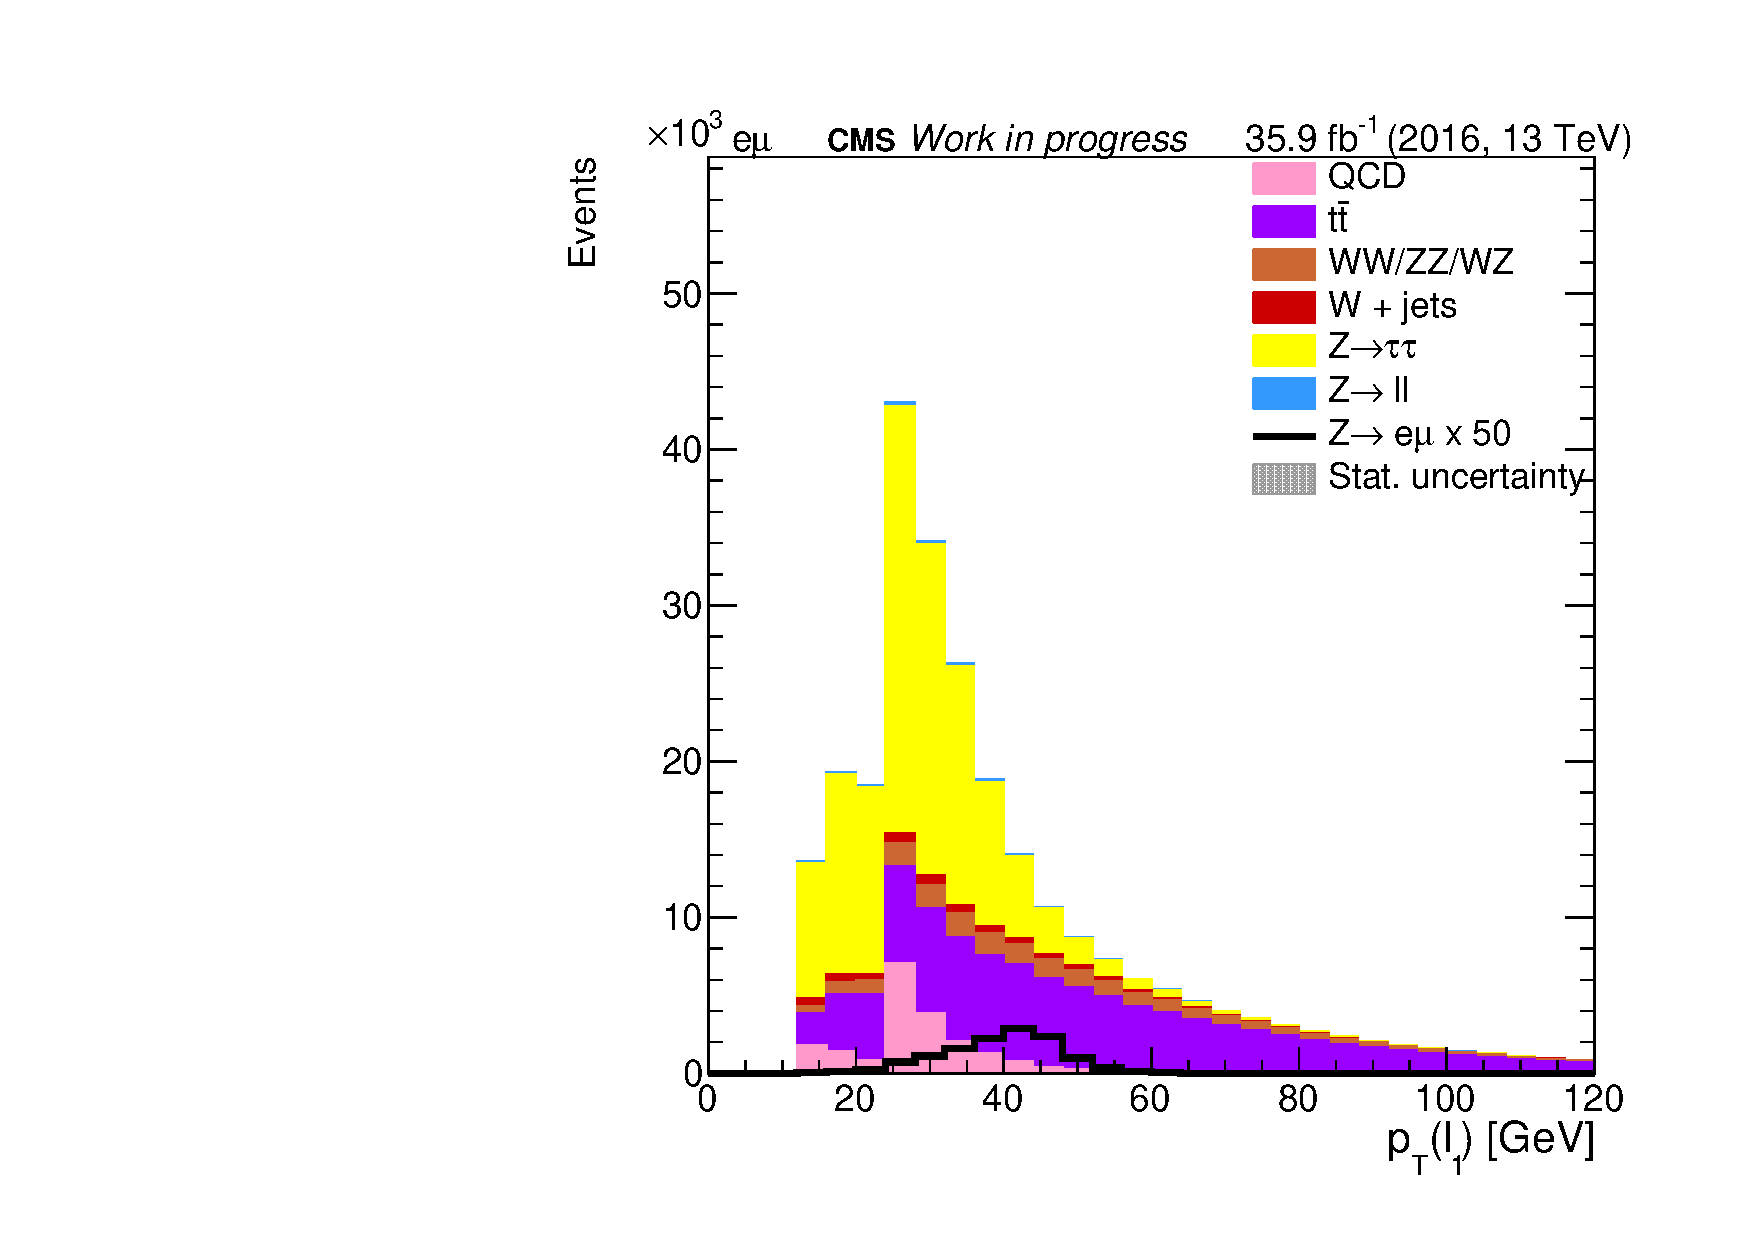
\includegraphics[width=0.45\textwidth]{plots/em/TransverseMomentum1_withsignal.pdf}

	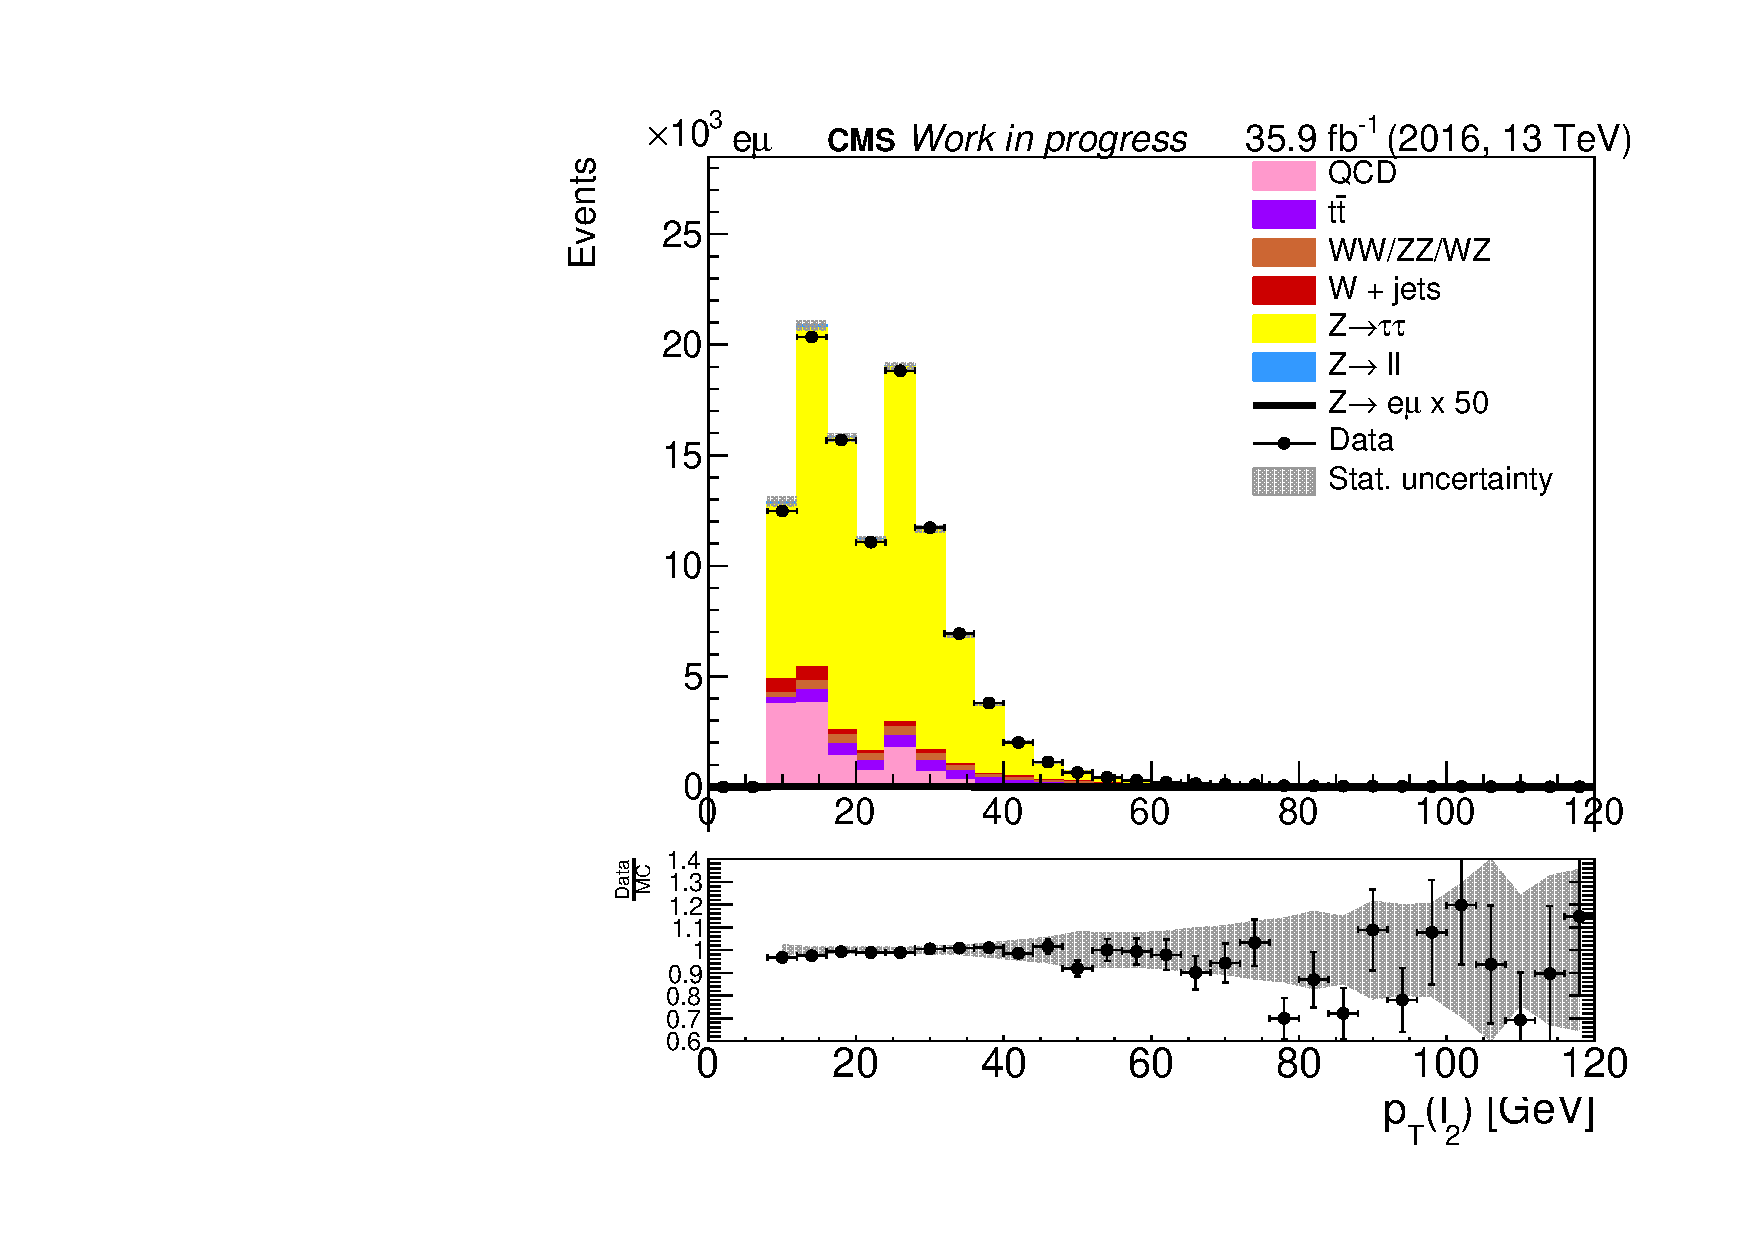
\includegraphics[width=0.45\textwidth]{plots/em/TransverseMomentum2_CR.pdf}
	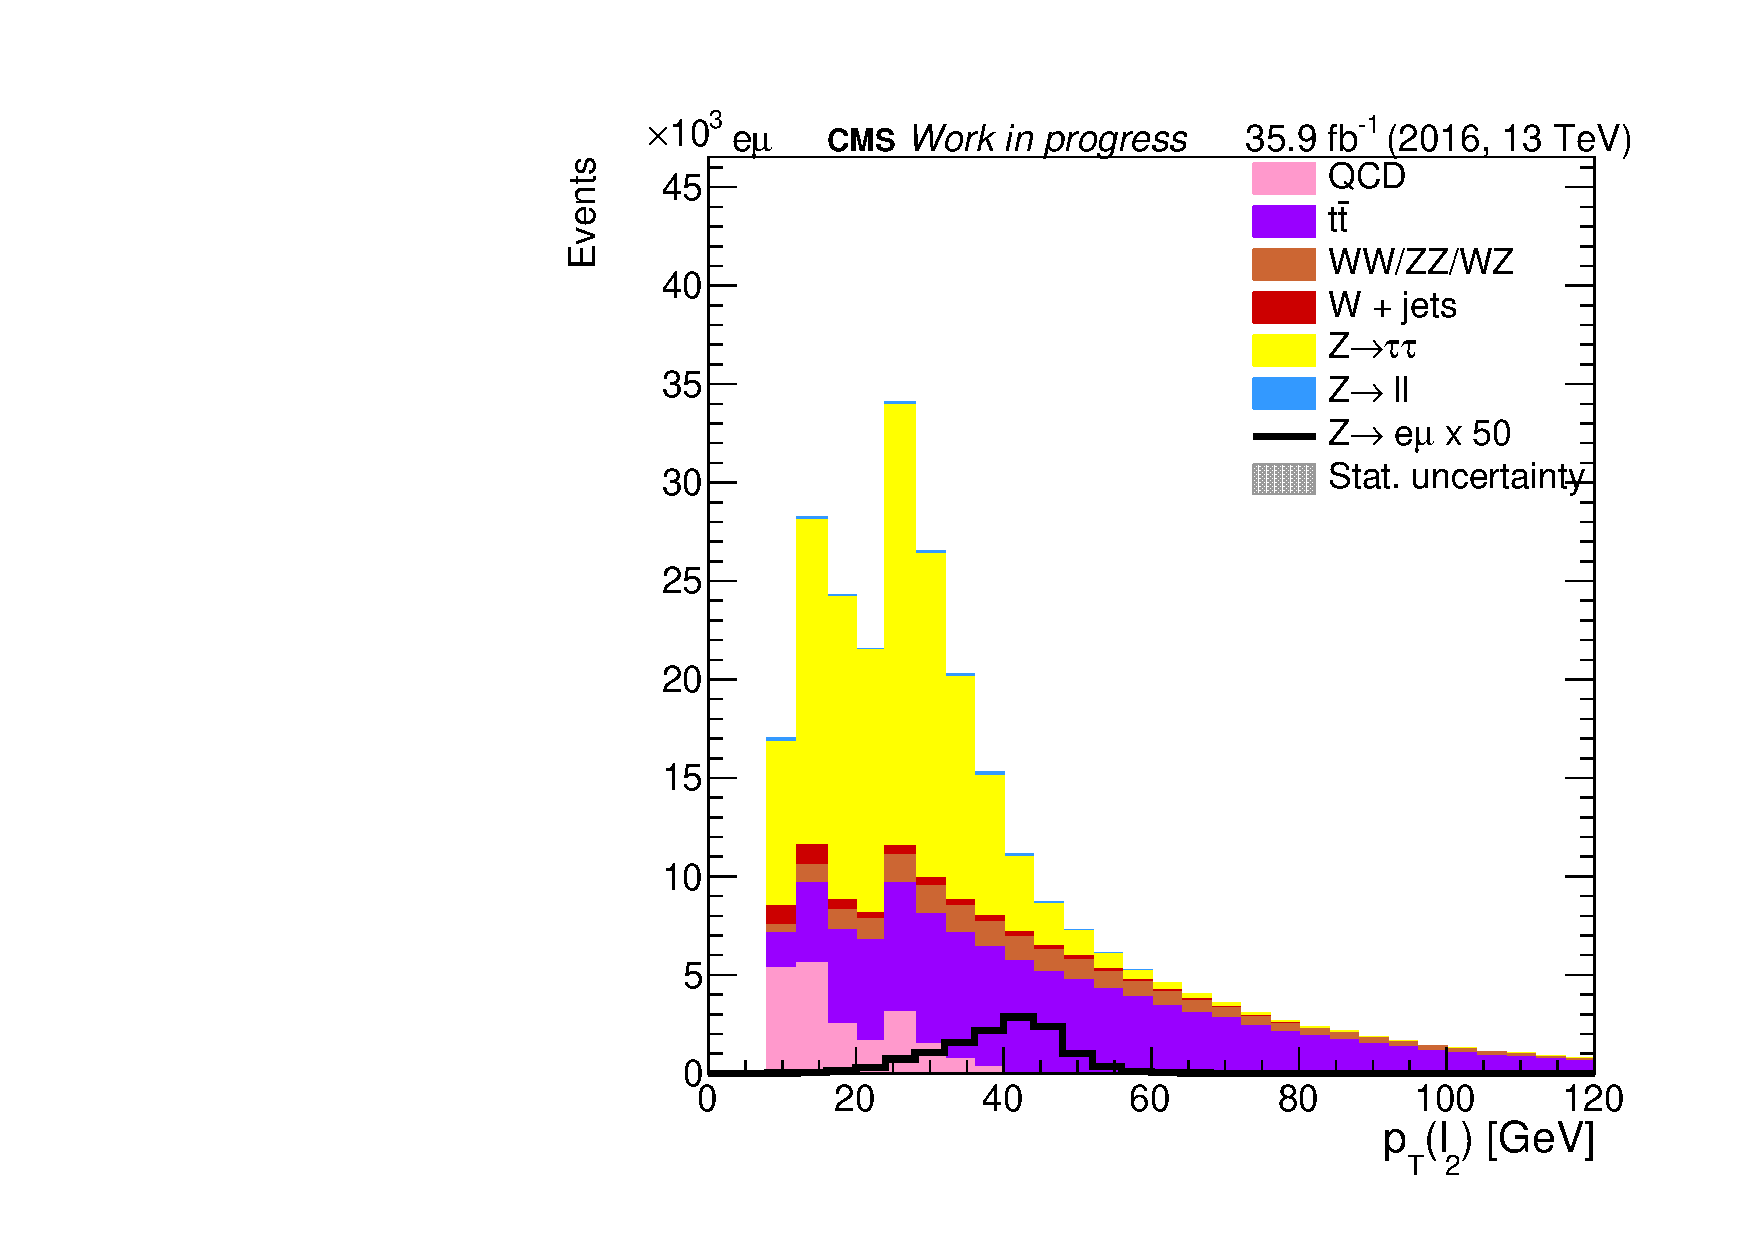
\includegraphics[width=0.45\textwidth]{plots/em/TransverseMomentum2_withsignal.pdf}
\end{figure}


\begin{figure}[htp]
	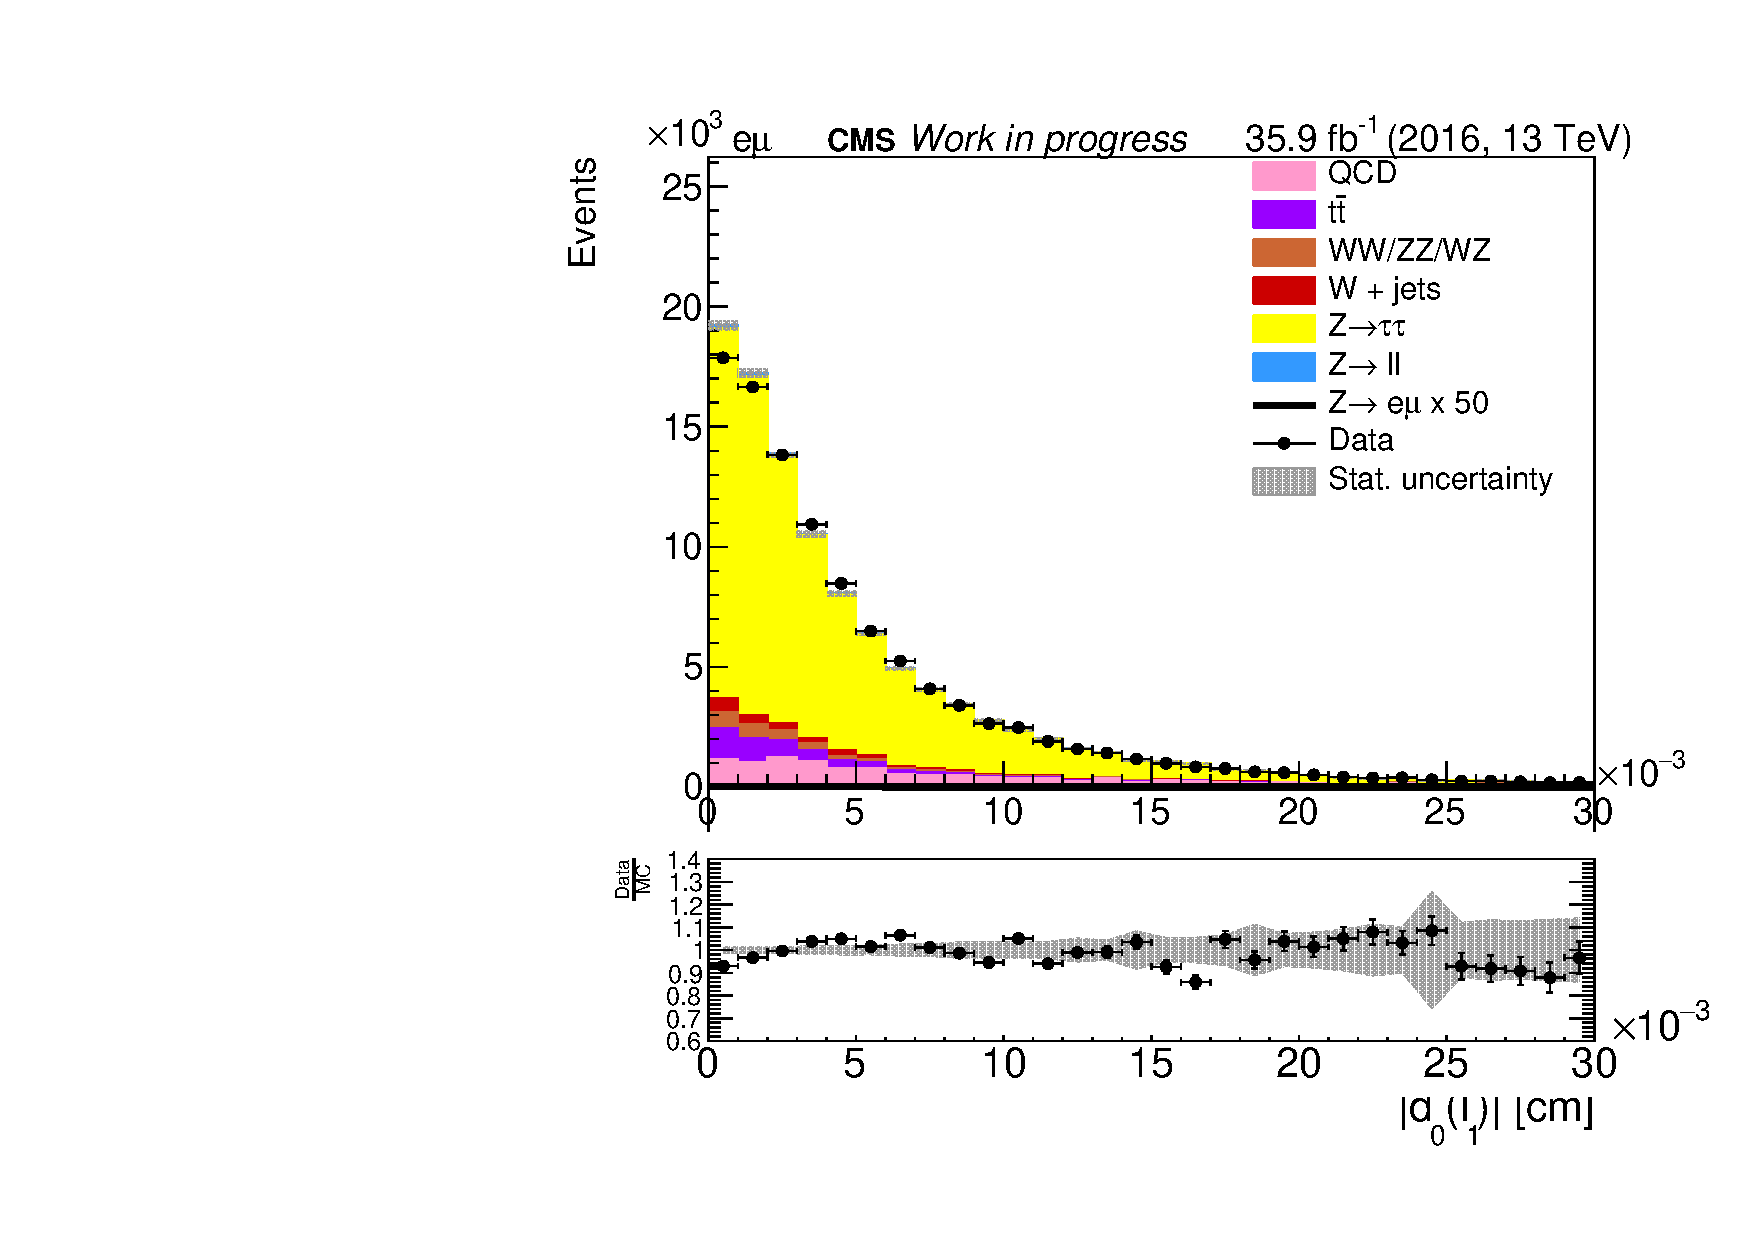
\includegraphics[width=0.45\textwidth]{plots/em/ImpactParameter1_CR.pdf}
	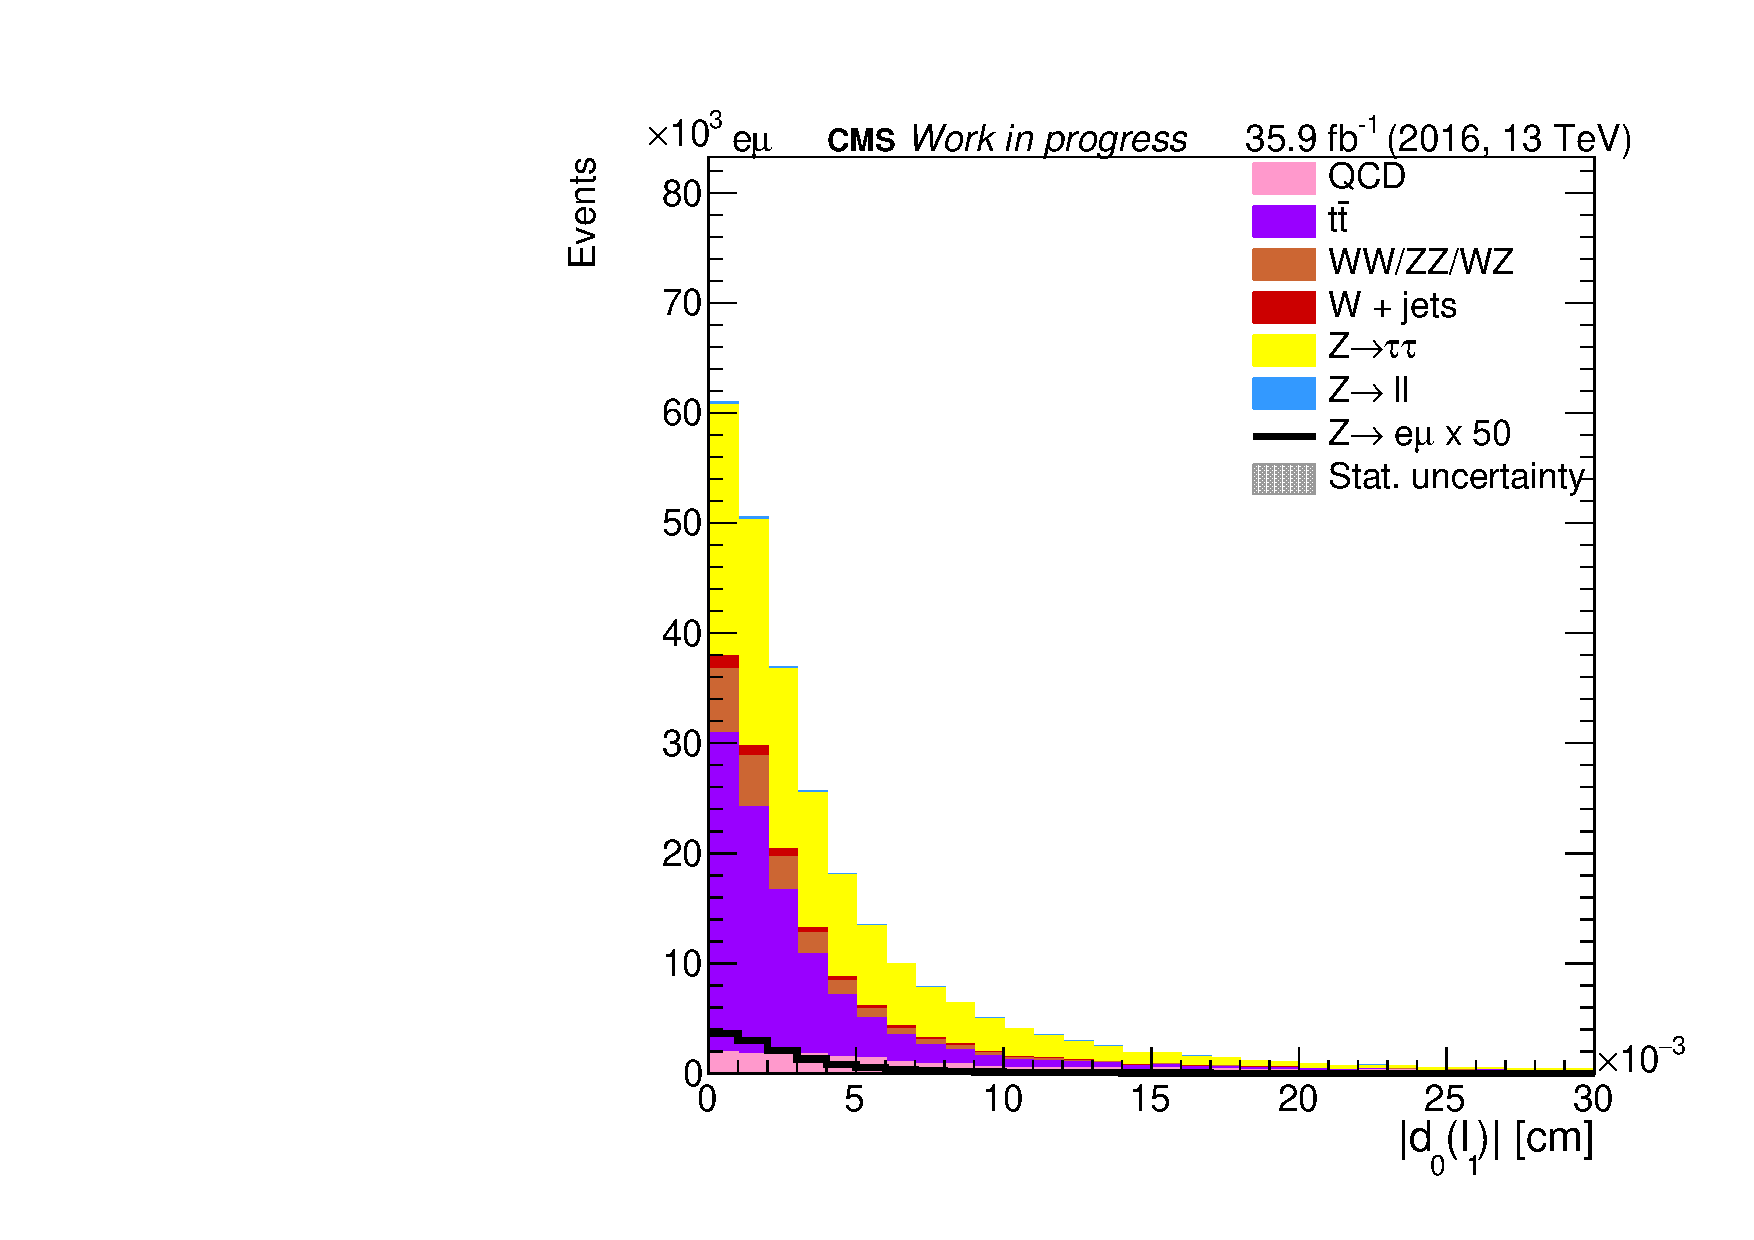
\includegraphics[width=0.45\textwidth]{plots/em/ImpactParameter1_withsignal.pdf}

	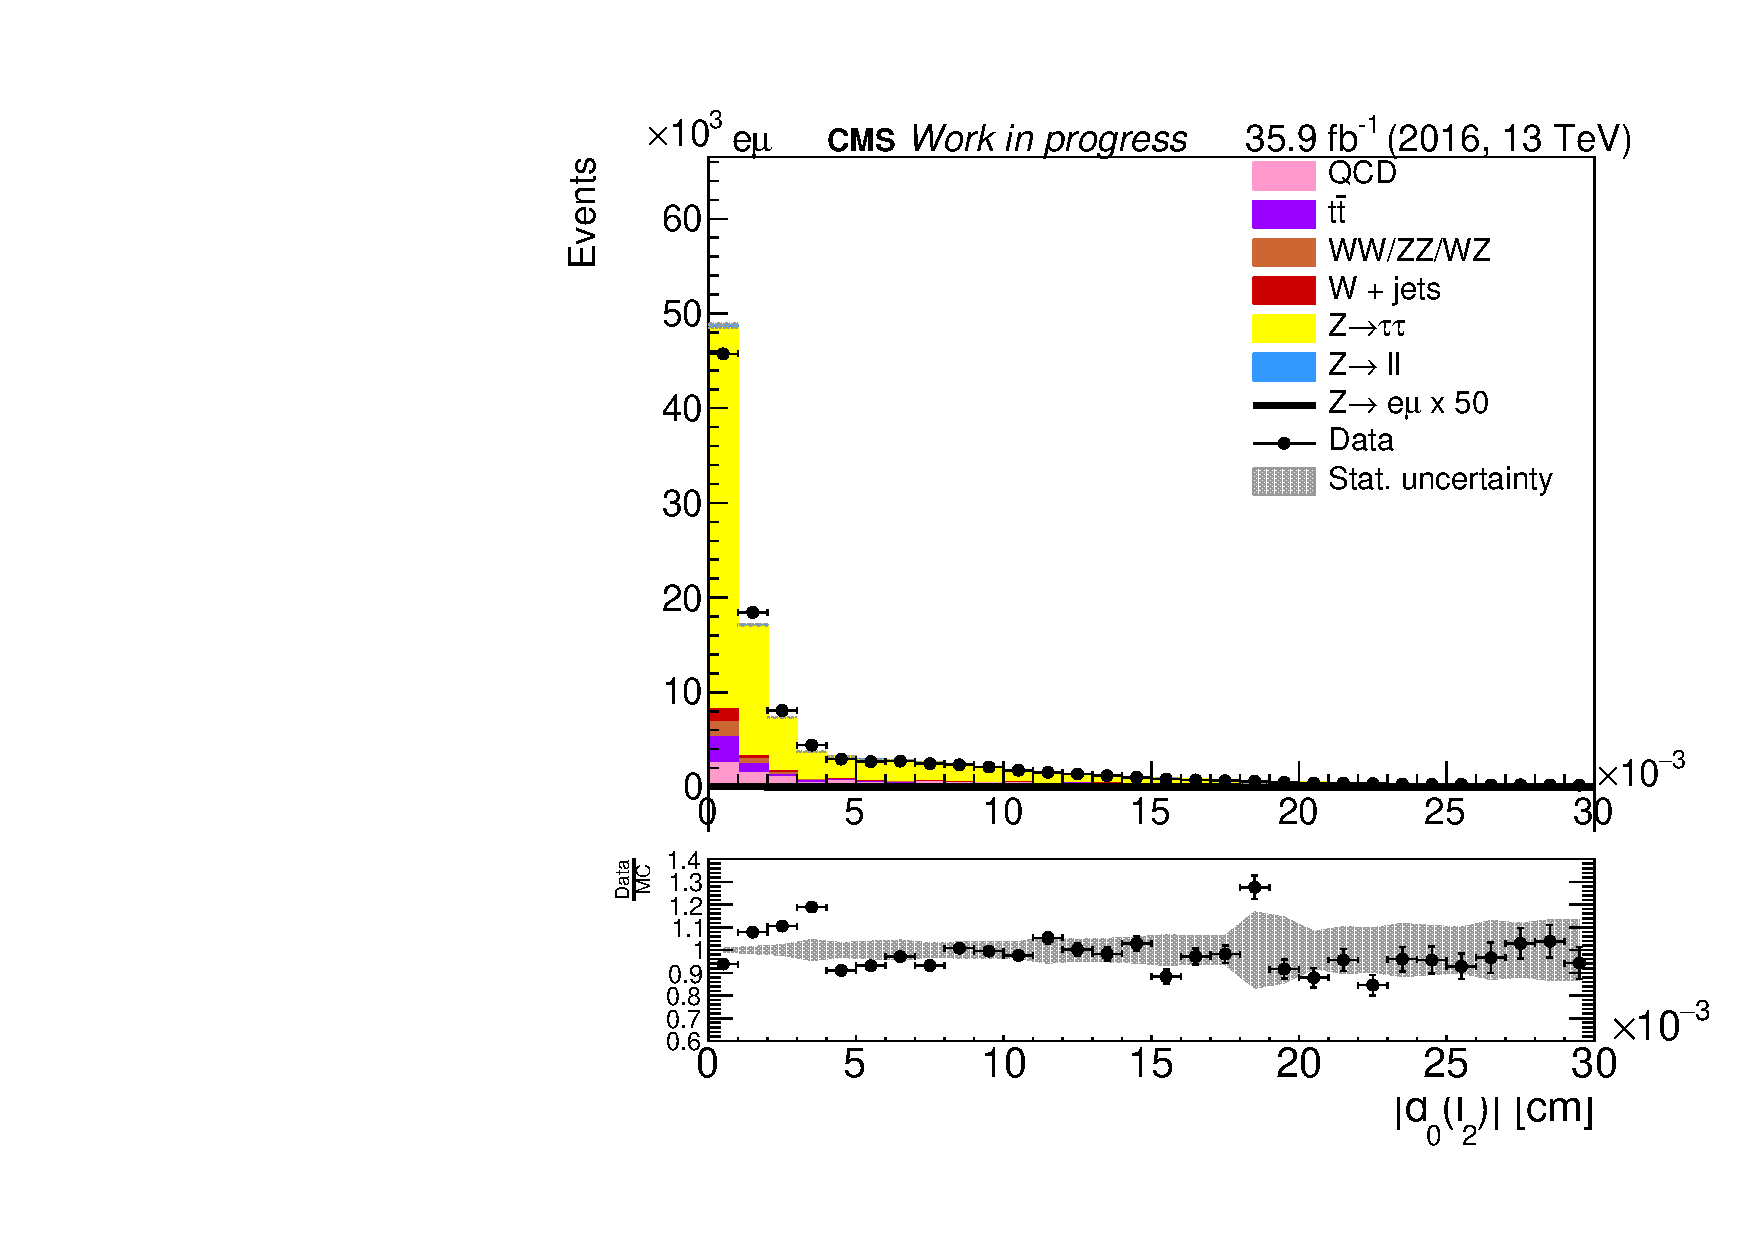
\includegraphics[width=0.45\textwidth]{plots/em/ImpactParameter2_CR.pdf}
	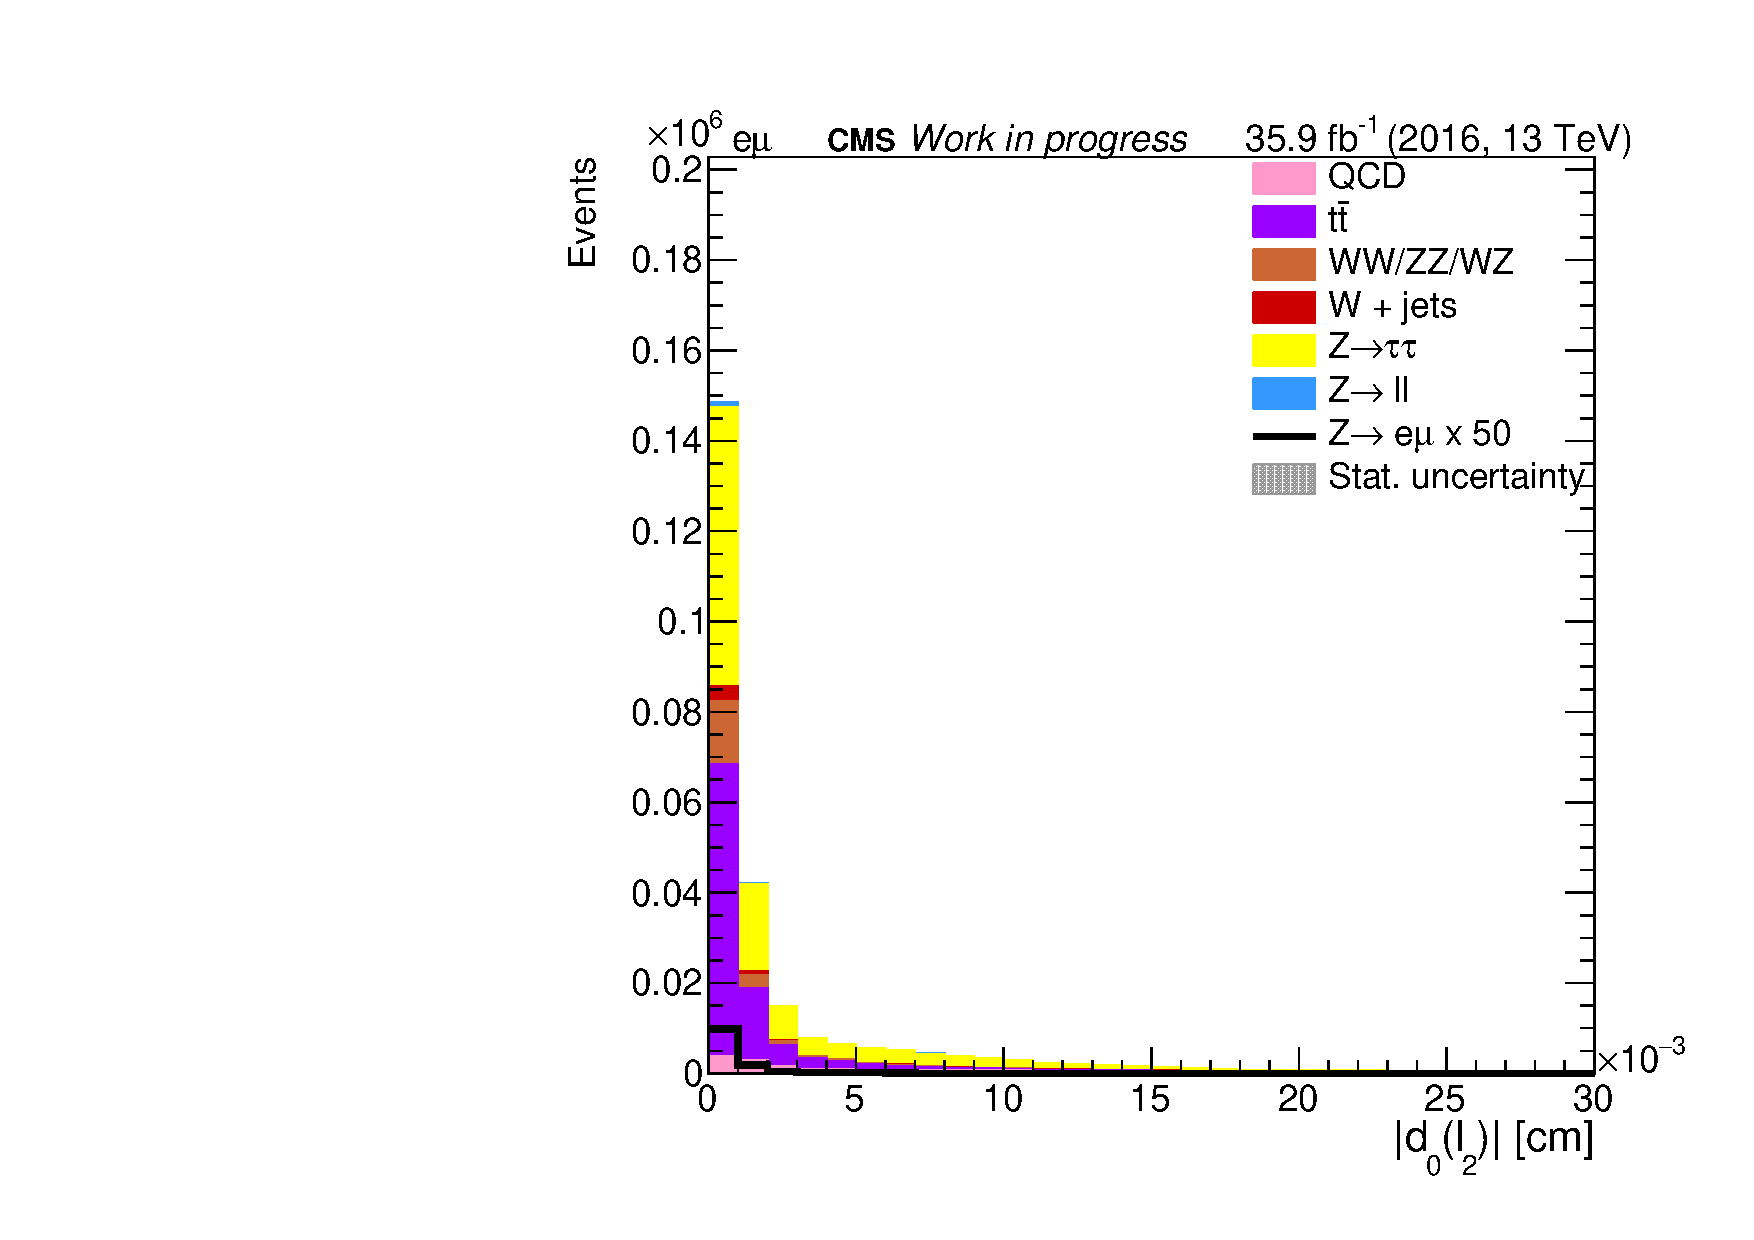
\includegraphics[width=0.45\textwidth]{plots/em/ImpactParameter2_withsignal.pdf}

	\includegraphics[width=0.45\textwidth]{plots/em/MissingTranverseEnergy_CR.pdf}
	\includegraphics[width=0.45\textwidth]{plots/em/MissingTranverseEnergy_withsignal.pdf}
\end{figure}

\newpage

\section*{Plot for the $e\tau$ final state}

\begin{figure}[htp]
	\includegraphics[width=0.45\textwidth]{plots/et/DeltaPhiL1L2_CR.pdf}
	\includegraphics[width=0.45\textwidth]{plots/et/DeltaPhiL1L2_withsignal.pdf}

	\includegraphics[width=0.45\textwidth]{plots/et/DeltaPhiL1Z_CR.pdf}
	\includegraphics[width=0.45\textwidth]{plots/et/DeltaPhiL1Z_withsignal.pdf}

\end{figure}


\begin{figure}[htp]
	\includegraphics[width=0.45\textwidth]{plots/et/DeltaPhiL2Z_CR.pdf}
	\includegraphics[width=0.45\textwidth]{plots/et/DeltaPhiL2Z_withsignal.pdf}

	\includegraphics[width=0.45\textwidth]{plots/et/DeltaPhiMetL1_CR.pdf}
	\includegraphics[width=0.45\textwidth]{plots/et/DeltaPhiMetL1_withsignal.pdf}

	\includegraphics[width=0.45\textwidth]{plots/et/DeltaPhiMetL2_CR.pdf}
	\includegraphics[width=0.45\textwidth]{plots/et/DeltaPhiMetL2_withsignal.pdf}
\end{figure}


\begin{figure}[htp]
	\includegraphics[width=0.45\textwidth]{plots/et/DiEta_CR.pdf}
	\includegraphics[width=0.45\textwidth]{plots/et/DiEta_withsignal.pdf}

	\includegraphics[width=0.45\textwidth]{plots/et/DiLepPt_CR.pdf}
	\includegraphics[width=0.45\textwidth]{plots/et/DiLepPt_withsignal.pdf}

	\includegraphics[width=0.45\textwidth]{plots/et/DiTransverseMass_CR.pdf}
	\includegraphics[width=0.45\textwidth]{plots/et/DiTransverseMass_withsignal.pdf}
\end{figure}


\begin{figure}[htp]
	\includegraphics[width=0.45\textwidth]{plots/et/EnergySum_CR.pdf}
	\includegraphics[width=0.45\textwidth]{plots/et/EnergySum_withsignal.pdf}

	\includegraphics[width=0.45\textwidth]{plots/et/TransverseMomentum1_CR.pdf}
	\includegraphics[width=0.45\textwidth]{plots/et/TransverseMomentum1_withsignal.pdf}

	\includegraphics[width=0.45\textwidth]{plots/et/TransverseMomentum2_CR.pdf}
	\includegraphics[width=0.45\textwidth]{plots/et/TransverseMomentum2_withsignal.pdf}
\end{figure}


\begin{figure}[htp]
	\includegraphics[width=0.45\textwidth]{plots/et/ImpactParameter1_CR.pdf}
	\includegraphics[width=0.45\textwidth]{plots/et/ImpactParameter1_withsignal.pdf}

	\includegraphics[width=0.45\textwidth]{plots/et/ImpactParameter2_CR.pdf}
	\includegraphics[width=0.45\textwidth]{plots/et/ImpactParameter2_withsignal.pdf}

	\includegraphics[width=0.45\textwidth]{plots/et/MissingTranverseEnergy_CR.pdf}
	\includegraphics[width=0.45\textwidth]{plots/et/MissingTranverseEnergy_withsignal.pdf}
\end{figure}

\newpage

\section*{Plot for the $\mu\tau$ final state}

\begin{figure}[htp]
	\includegraphics[width=0.45\textwidth]{plots/mt/DeltaPhiL1L2_CR.pdf}
	\includegraphics[width=0.45\textwidth]{plots/mt/DeltaPhiL1L2_withsignal.pdf}

	\includegraphics[width=0.45\textwidth]{plots/mt/DeltaPhiL1Z_CR.pdf}
	\includegraphics[width=0.45\textwidth]{plots/mt/DeltaPhiL1Z_withsignal.pdf}

\end{figure}


\begin{figure}[htp]
	\includegraphics[width=0.45\textwidth]{plots/mt/DeltaPhiL2Z_CR.pdf}
	\includegraphics[width=0.45\textwidth]{plots/mt/DeltaPhiL2Z_withsignal.pdf}

	\includegraphics[width=0.45\textwidth]{plots/mt/DeltaPhiMetL1_CR.pdf}
	\includegraphics[width=0.45\textwidth]{plots/mt/DeltaPhiMetL1_withsignal.pdf}

	\includegraphics[width=0.45\textwidth]{plots/mt/DeltaPhiMetL2_CR.pdf}
	\includegraphics[width=0.45\textwidth]{plots/mt/DeltaPhiMetL2_withsignal.pdf}
\end{figure}


\begin{figure}[htp]
	\includegraphics[width=0.45\textwidth]{plots/mt/DiEta_CR.pdf}
	\includegraphics[width=0.45\textwidth]{plots/mt/DiEta_withsignal.pdf}

	\includegraphics[width=0.45\textwidth]{plots/mt/DiLepPt_CR.pdf}
	\includegraphics[width=0.45\textwidth]{plots/mt/DiLepPt_withsignal.pdf}

	\includegraphics[width=0.45\textwidth]{plots/mt/DiTransverseMass_CR.pdf}
	\includegraphics[width=0.45\textwidth]{plots/mt/DiTransverseMass_withsignal.pdf}
\end{figure}


\begin{figure}[htp]
	\includegraphics[width=0.45\textwidth]{plots/mt/EnergySum_CR.pdf}
	\includegraphics[width=0.45\textwidth]{plots/mt/EnergySum_withsignal.pdf}

	\includegraphics[width=0.45\textwidth]{plots/mt/TransverseMomentum1_CR.pdf}
	\includegraphics[width=0.45\textwidth]{plots/mt/TransverseMomentum1_withsignal.pdf}

	\includegraphics[width=0.45\textwidth]{plots/mt/TransverseMomentum2_CR.pdf}
	\includegraphics[width=0.45\textwidth]{plots/mt/TransverseMomentum2_withsignal.pdf}
\end{figure}


\begin{figure}[htp]
	\includegraphics[width=0.45\textwidth]{plots/mt/ImpactParameter1_CR.pdf}
	\includegraphics[width=0.45\textwidth]{plots/mt/ImpactParameter1_withsignal.pdf}

	\includegraphics[width=0.45\textwidth]{plots/mt/ImpactParameter2_CR.pdf}
	\includegraphics[width=0.45\textwidth]{plots/mt/ImpactParameter2_withsignal.pdf}

	\includegraphics[width=0.45\textwidth]{plots/mt/MissingTranverseEnergy_CR.pdf}
	\includegraphics[width=0.45\textwidth]{plots/mt/MissingTranverseEnergy_withsignal.pdf}
\end{figure}


\end{appendices}

\printglossaries

\pagestyle{bibliography}
\bibliographystyle{packages/bibstyle.bst}
\bibliography{bibliography.bib}  
\addcontentsline{toc}{chapter}{Bibliography}

\end{document}
